A fit to the \mll distribution is performed in search of the characteristic edge signature described in section~\ref{sec:somesignalsection}. Different functions are used to model the contributions of the potential signal, flavour-symmetric backgrounds, and backgrounds containing a Z boson. To fully exploit the available information, an unbinned maximum-likelihood fit is performed simultaneously to the \EE, \MM, and \EM event samples for both the signal and forward dilepton selection in the signal region.

\section{Background and signal models}



\subsection{Model for Z backgrounds}
\label{sec:Zmodel}
The background model for events containing a Z boson contains of two components: one model for the Z boson peak and one for the contribution of the Drell--Yan continuum. The latter one is a simple falling exponential. The peak model consists of a Breit-Wigner function with mean and widths fixed to the DPG values for the Z boson, convolved with a double-sided crystal ball function~\cite{Crystal}. The first component models the physical peak while the latter accounts for the detector resolution and radiative corrections to the Z lineshape. The double-sided crystal ball itself consists of a Gaussian core and exponential falloffs to both sides of the peak, parametrized as
\begin{eqnarray*}
\mathcal{P}_{DSCB}(m_{\ell\ell}) = \begin{cases} A_{1} (B_{1}-\frac{m_{ll}-\mu_{CB}}{\sigma_{CB}})^{-n_{1}} &\mbox{if } \frac{m_{ll}-\mu_{CB}}{\sigma_{CB}}<-\alpha_{1} \\
\textrm{exp}\left(-\frac{(m_{ll}-\mu_{CB})^2}{2\sigma_{CB}^2}\right) &\mbox{if } -\alpha_{1}<\frac{m_{ll}-\mu_{CB}}{\sigma_{CB}}<\alpha_{2} \\
A_{2} (B_{2}+\frac{m_{ll}-\mu_{CB}}{\sigma_{CB}})^{-n_{2}} &\mbox{if } \frac{m_{ll}-\mu_{CB}}{\sigma_{CB}}>\alpha_{2} \\
\end{cases}
\end{eqnarray*}
where $\sigma_{CB}$ and $\mu_{CB}$ are the parameters of the central Gaussian and the $n_i$ and $\alpha_i$ govern the transition to and the shape of the exponential falloff. The $A_i$ and $B_i$ are substitutions for
\begin{eqnarray*}
A_{i} = \left(\frac{n_{i}}{|\alpha_{i}|}\right)^{n_{i}} \cdot \textrm{exp}\left(-\frac{|\alpha_{i}|^2}{2}\right) \quad \textrm{and}\quad B_{i} = \frac{n_{i}}{|\alpha_{i}|}-|\alpha_{i}| .
\end{eqnarray*}
Taking into account also the exponential function described the Drell--Yan continuum, the full description is therefore 
\begin{eqnarray*}
\mathcal{P}_{DY} (m_{\ell\ell}) = (1-f_{exp})\mathcal{P}_{exp}(m_{\ell\ell})+ f_{exp}\int \mathcal{P}_{DSCB}(m_{\ell\ell})\mathcal{P}_{BW}(m_{\ell\ell}-m') dm',
\end{eqnarray*}
where $f_{exp}$ is the fraction that the exponential component contributes to the full PDF. A full list of the parameters of the model is given in Table~\ref{tab:Fit_Par_Overview_Z}.


\begin{table}[htbp]
\begin{center}
 \renewcommand{\arraystretch}{1.3}
 \caption{List of all parameters of the model for Drell--Yan backgrounds for the fit in the Drell--Yan control region. Given are intial values, allowed ranges and the status of the parameters. A set of these parameters exists for both the central and forward dilepton selection.\label{tab:Fit_Par_Overview_Z}}
\begin{tabular}{l|c|c|c|c|ccccccccccccccccccccc}
& parameter & status & initial value & minimum & maximum \\ \hline
\multirow{10}{*}{$\mathbf{p}_{Z}^{ee}$} & $m_{\mathrm{Z}} [\mathrm{GeV}]$ & fixed & 91.1876 & - & - \\ 
& $\sigma_{\mathrm{Z}}  [\mathrm{GeV}]$ & fixed & 2.4952 & - & - \\
& $\mu_{CB}^{ee} [\mathrm{GeV}]$ & floating & 3.0 & -10 & 10 \\ 
& $\sigma_{CB}^{ee}$ & floating & 1.6 & 0 & 20 \\
& $\alpha_{1}^{ee}$ & floating & 1.16 & 0 & 10 \\
& $\alpha_{2}^{ee}$ & floating & 2.5 & 0 & 10 \\
& $n_{1}^{ee}$ & floating & 2.9 & 0 & 20 \\
& $n_{2}^{ee}$ & floating & 1.04 & 0 & 20 \\
& $f_{exp}^{ee}$ & floating & 0.9 & 0 & 1 \\
& $\mu_{exp}^{ee} [\mathrm{GeV}^{-1}]$ & floating & -0.02& -0.1 & 0 \\ \hline
\multirow{10}{*}{$\mathbf{p}_{Z}^{\mu\mu}$} & $m_{\mathrm{Z}} [\mathrm{GeV}]$ & fixed & 91.1876 & - & - \\ 
& $\sigma_{\mathrm{Z}} [\mathrm{GeV}]$  & fixed & 2.4952 & - & - \\
& $\mu_{CB}^{\mu\mu} [\mathrm{GeV}]$ & floating & 3.0 & -10 & 10 \\
&  $\sigma_{CB}^{\mu\mu}$ & floating & 1.6 & 0 & 20 \\
&  $\alpha_{1}^{\mu\mu}$ & floating & 1.16 & 0 & 10 \\
&  $\alpha_{2}^{\mu\mu}$ & floating & 2.5 & 0 & 10 \\
&  $n_{1}^{\mu\mu}$ & floating & 2.9 & 0 & 20 \\
&  $n_{2}^{\mu\mu}$ & floating & 1.04 & 0 & 20 \\
&  $f_{exp}^{\mu\mu}$ & floating & 0.9 & 0 & 1 \\
&  $\mu_{exp}^{\mu\mu} [\mathrm{GeV}^{-1}]$& floating & -0.02 & -0.1 & 0 \\ 
\end{tabular}

\end{center}
\end{table}


This model is fitted to the data in the Drell--Yan control region separately for \EE and \MM events after flavour-symmetric backgrounds are subtracted using OF events. Afterwards, all parameters of the model are fixed and only the normalization is left floating in the fit in the signal region. The resulting fits are shown in Figure~\ref{fig:dyFits} and are a good description of the distribution in all cases. 

\begin{figure}[htbp]
\centering
\begin{minipage}[t]{0.49\textwidth}
  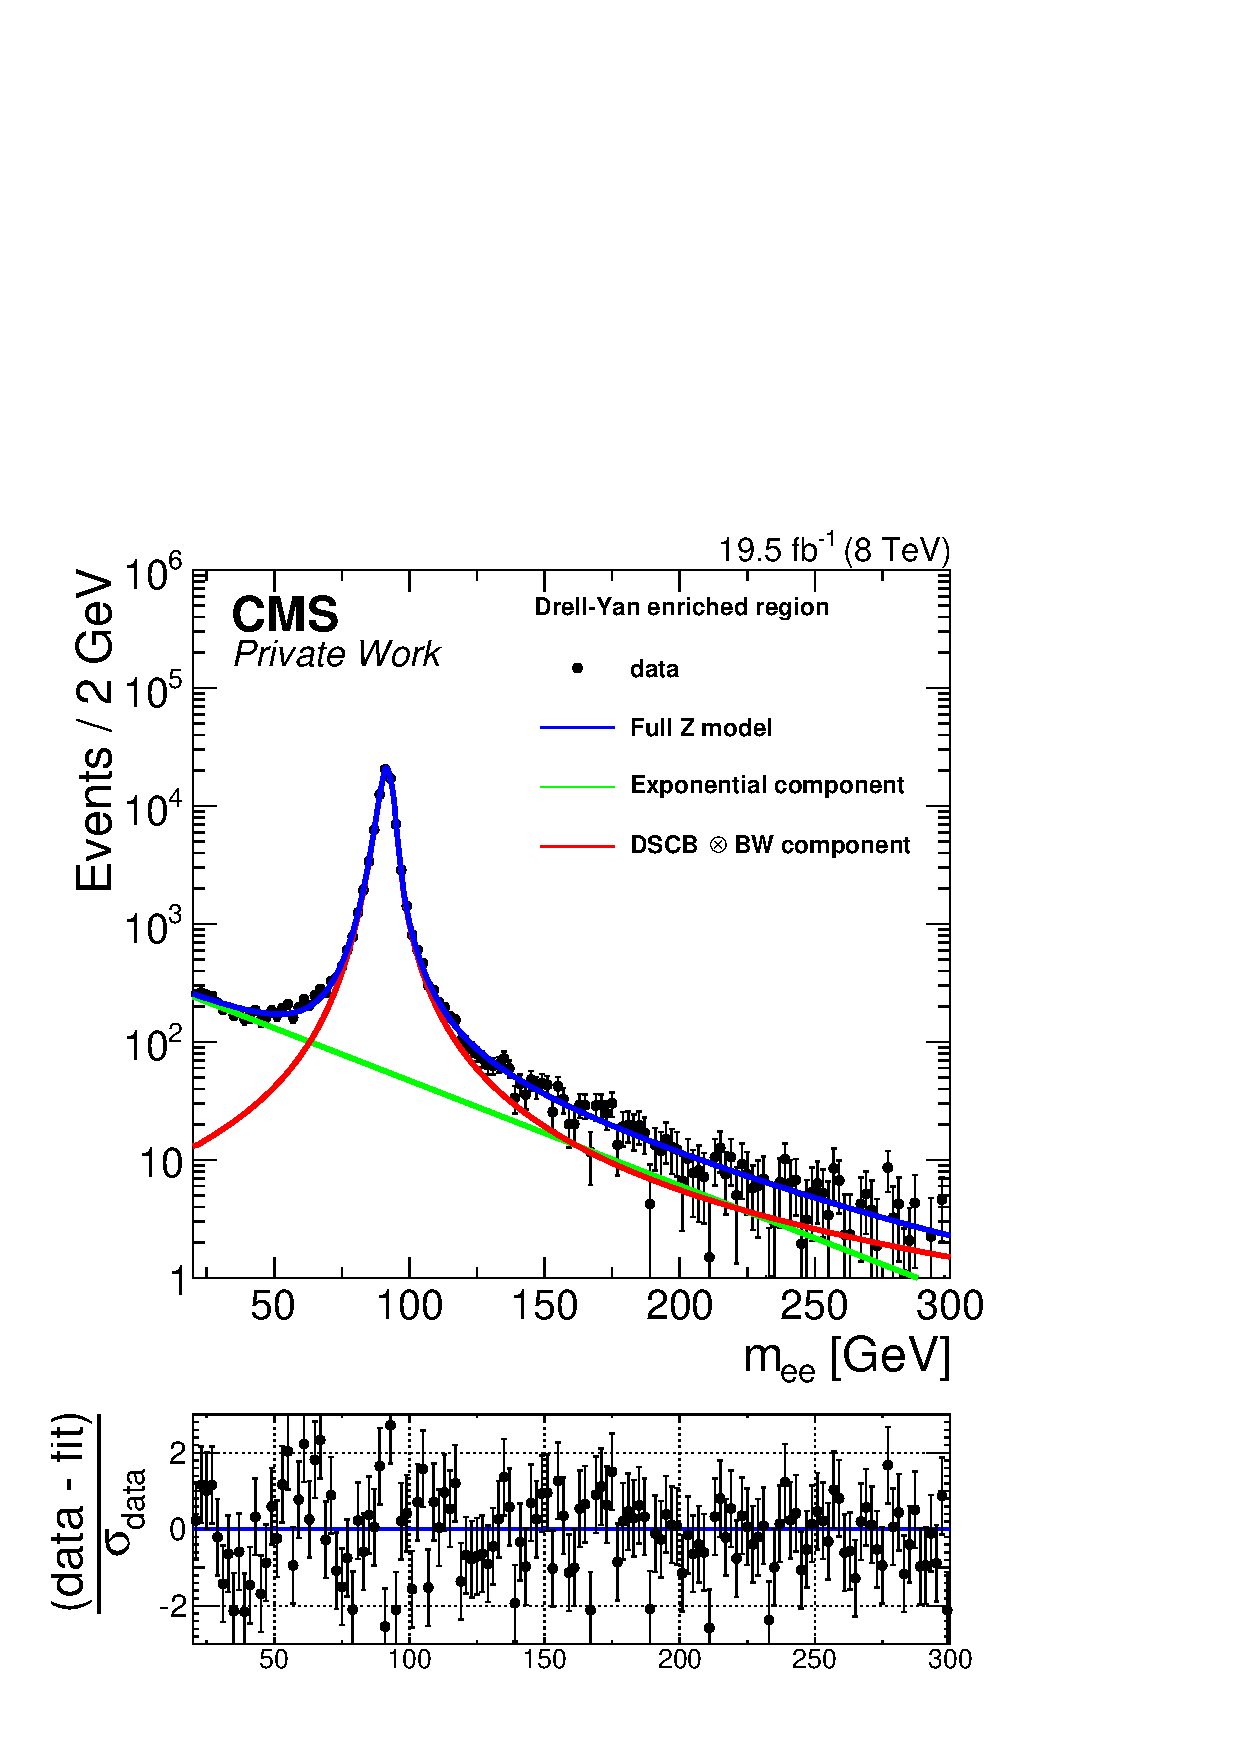
\includegraphics[width=\textwidth]{plots/results/fit/expoFitEE_Log_Central.pdf}
\end{minipage}
\begin{minipage}[t]{0.49\textwidth}
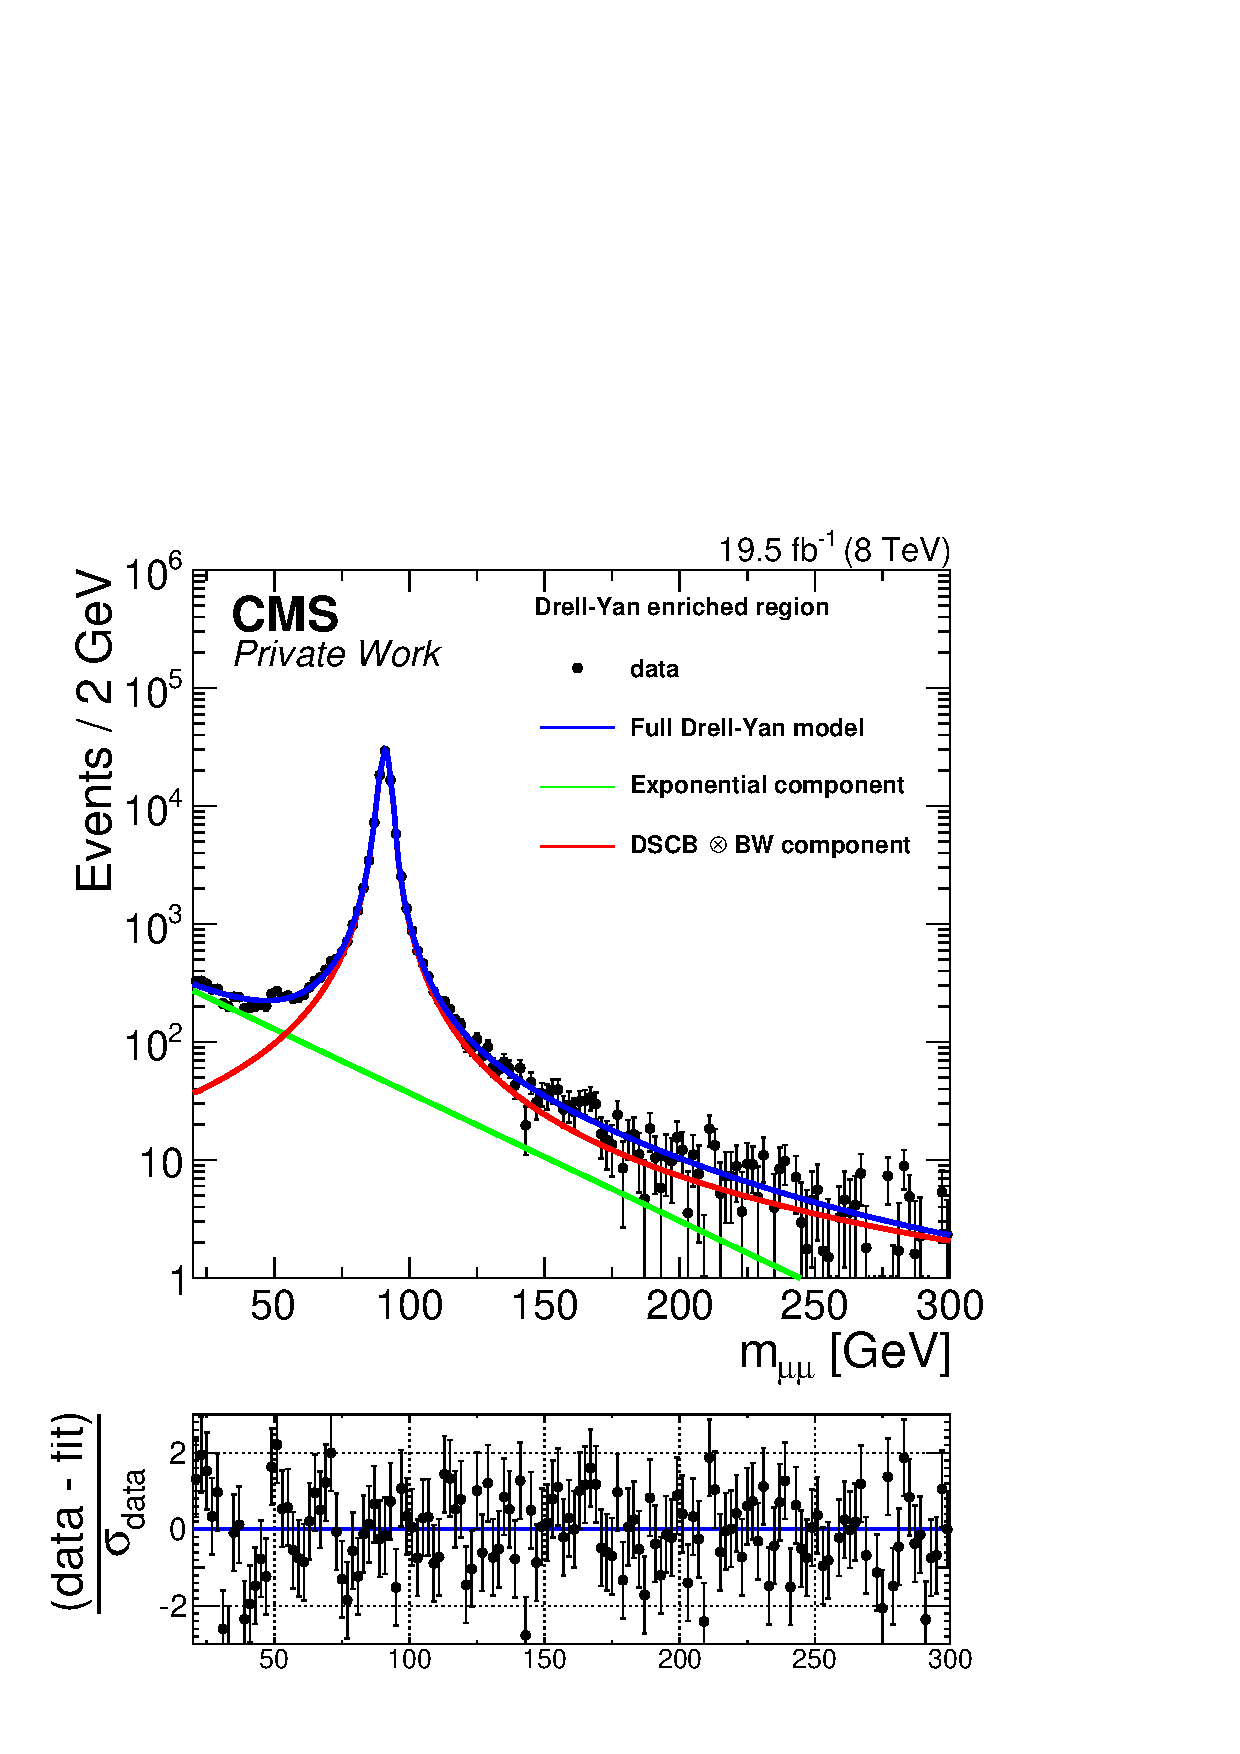
\includegraphics[width=\textwidth]{plots/results/fit/expoFitMM_Log_Central.pdf}
\end{minipage}
\begin{minipage}[t]{0.49\textwidth}
  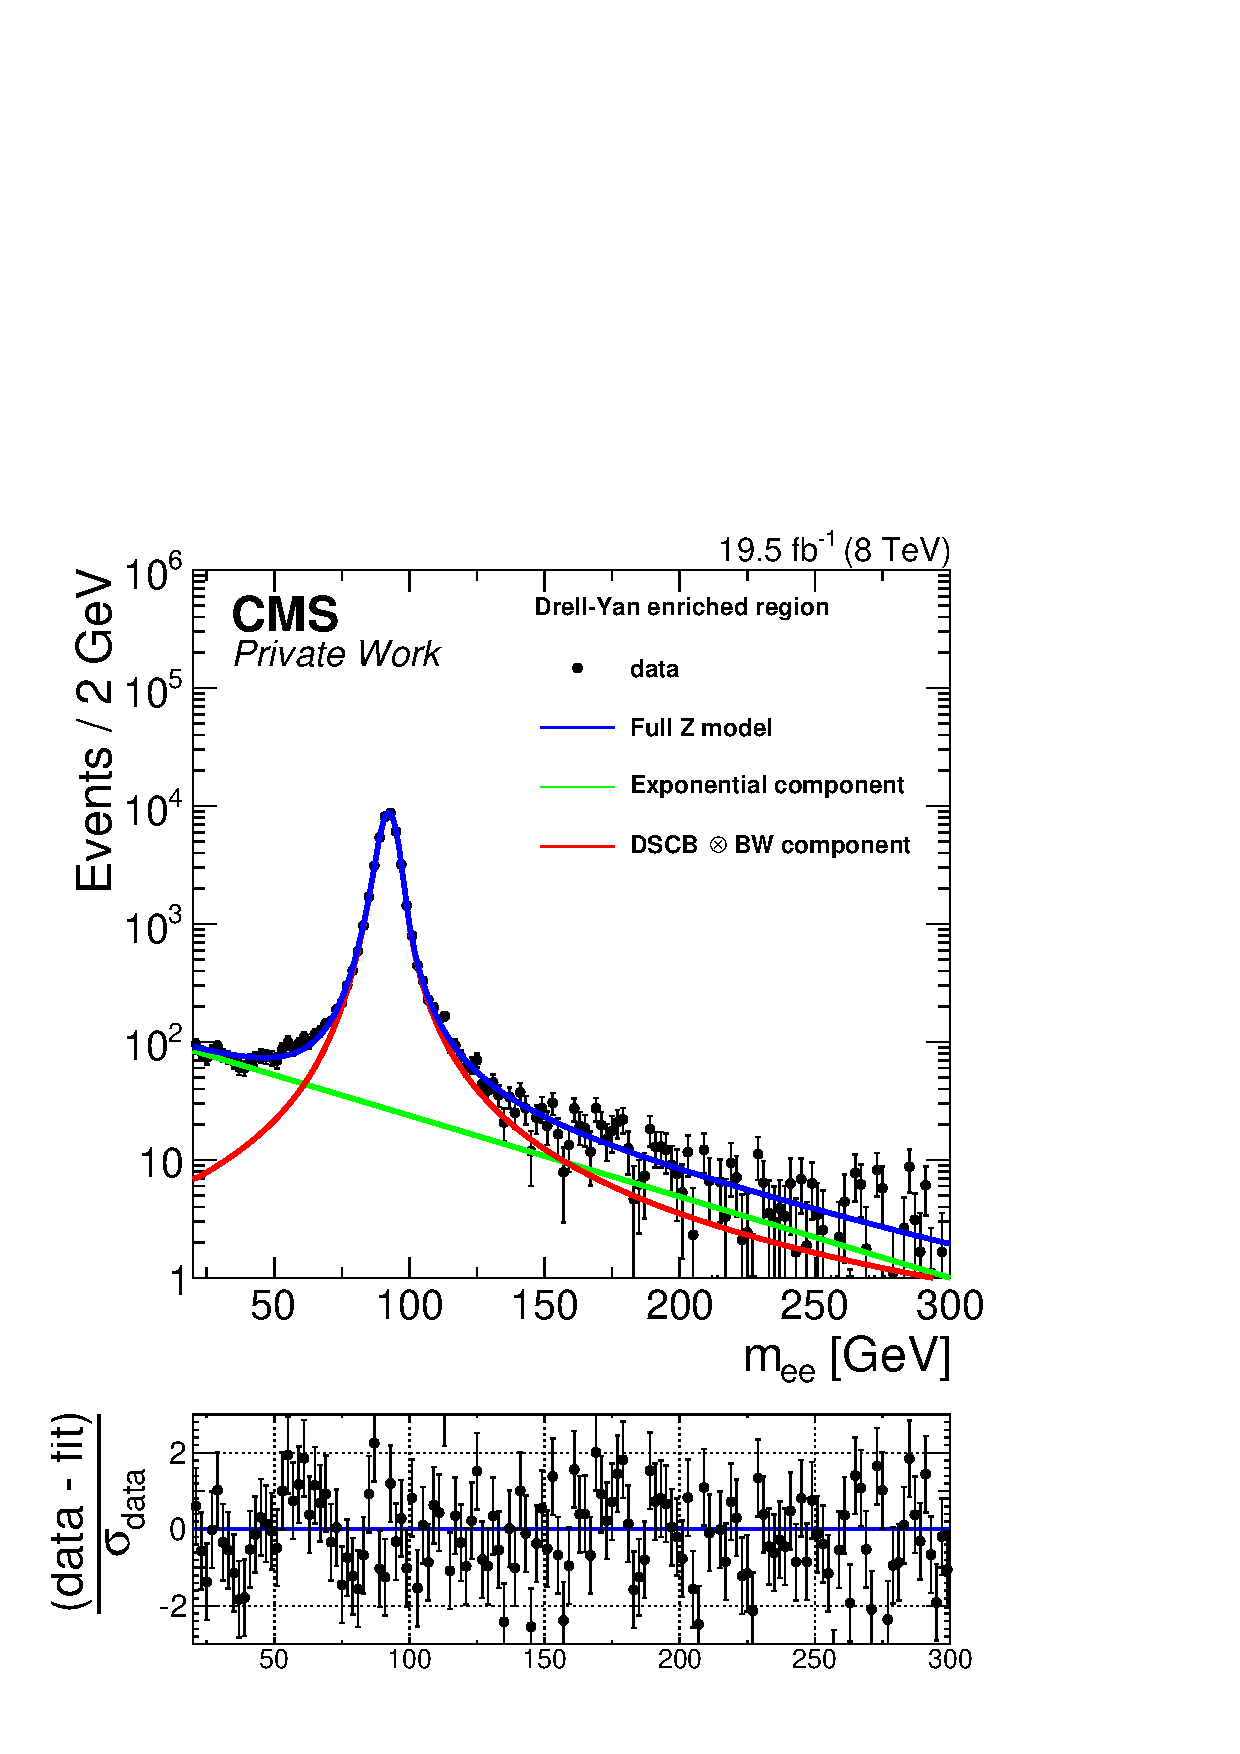
\includegraphics[width=\textwidth]{plots/results/fit/expoFitEE_Log_Forward.pdf}
\end{minipage}
\begin{minipage}[t]{0.49\textwidth}
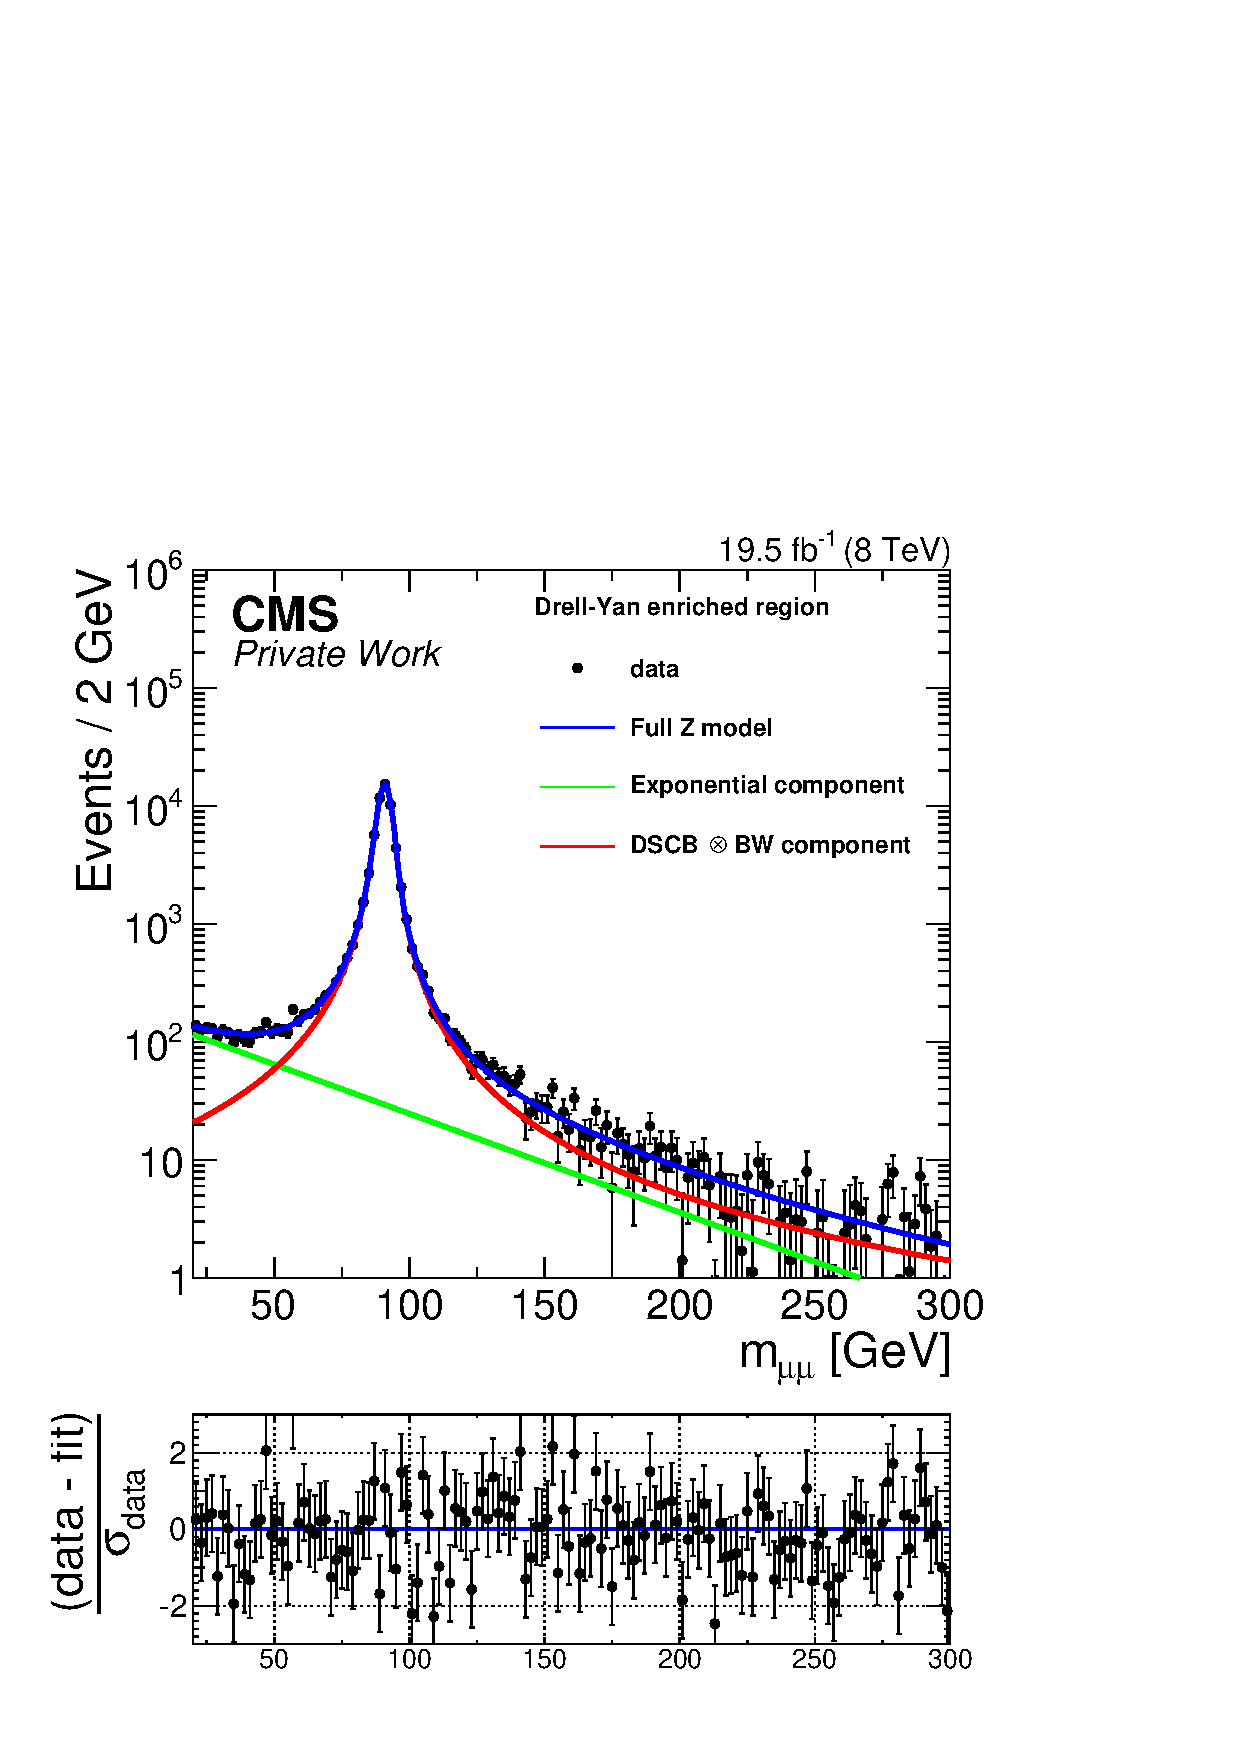
\includegraphics[width=\textwidth]{plots/results/fit/expoFitMM_Log_Forward.pdf}
\end{minipage}
\caption{Fit to the \mll distribution in the Drell--Yan control region separately for \EE (left) and \MM (right) events in the central (top) and forward (bottom) dilepton selection. The data is shown as black points while the resulting fit is shown in blue. The red and green lines show the contributions of the continuum model and the peak model to the combined fit.}
\label{fig:dyFits}
\end{figure}
From the Gaussian core component of the double-sided crystal ball the \mll resolution in the different channels is obtained, which is used as an input in the modelling of a potential signal. The resulting resolution values are shown in Table~\ref{tab:mllReso}. The fitted values range form about $\unit{1.4}{\giga\electronvolt}$ to $\unit{2.7}{\giga\electronvolt}$ depending on lepton flavour and rapidity. In general it is smaller for \MM pairs and for lepton pairs in the central part of the detector.  

\begin{table}
\centering
\caption{Fitted \mll resolution in the central and forward dilepton selections for \EE and \MM pairs.}
\label{tab:mllReso}
\begin{tabular}{l|c|c}
 & \EE & \MM \\
 \hline
 Central & $\unit{1.71\pm0.03}{\giga\electronvolt}$  & $\unit{1.44\pm0.01}{\giga\electronvolt}$\\
 Forward & $\unit{2.70\pm0.04}{\giga\electronvolt}$ & $\unit{2.01\pm0.03}{\giga\electronvolt}$\\

\end{tabular}
\end{table}






\subsection{Model for flavour-symmetric backgrounds}

\subsubsection{Nominal parametrization}
Flavour-symmetric models are described with a model consisting of three parts. The rising flank of the distribution is modelled with a power law, the peak region with a fourth order polynomial and the falling flank with an exponential falloff. 

\begin{eqnarray*}
{\mathcal{P}}_{FS}(m_{\ell\ell}) = \begin{cases} {\mathcal{P}}_{FSE,1}(m_{\ell\ell}) = c_{1} \cdot m_{\ell\ell}^{\alpha} &\mbox{if } 20\GeV < m_{\ell\ell} < m_{\ell\ell}^{(1)} \\
{\mathcal{P}}_{FS,2}(m_{\ell\ell}) = \sum_{i=0}^{3} c_{2,i} \cdot m_{\ell\ell}^{i} & \mbox{if } m_{\ell\ell}^{(1)}<m_{\ell\ell}<m_{\ell\ell}^{(2)} \\
{\mathcal{P}}_{FS,3}(m_{\ell\ell}) = c_{3}\cdot e^{-\beta m_{\ell\ell}} & \mbox{if } m_{\ell\ell}^{(2)}<m_{\ell\ell}<300\GeV \\
\end{cases} 
\end{eqnarray*}
where $m_{\ell\ell}^{(1)}$ and $m_{\ell\ell}^{(2)}$ are the transition points between the different parts of the model. The model is required to be normalized and also to be continuously differentiable in $m_{\ell\ell}^{(1)}$ and $m_{\ell\ell}^{(2)}$, reducing the number of free parameters to five. A full list of the parameters and their properties is given in Table~\ref{tab:Fit_Par_Overview_FS}.

\begin{table}[htbp]
\begin{center}
 \renewcommand{\arraystretch}{1.3}
 \caption{List of all parameters of the model for flavour-symmetric backgrounds. Given are intial values, allowed ranges and the status of the parameters. A set of these parameters exists for both the central and forward dilepton selection.\label{tab:Fit_Par_Overview_FS}}
\begin{tabular}{l|c|c|c|c|ccccccccccccccccccccc}
& parameter & status & initial value & minimum & maximum \\ \hline
\multirow{5}{*}{$\mathbf{p}_{FS}$} & $m_{\ell\ell}^{(1)} [\mathrm{GeV}]$ & floating & 50 & 20 & 80 \\ 
& $m_{\ell\ell}^{(2)}  [\mathrm{GeV}]$ & floating & 120 & 100 & 160 \\
& $c_{2,0}$ & floating & -1800 & -5000 & 5000 \\ 
& $c_{2,1}$ & floating & 120 & -400 & 400 \\
& $c_{2,2}$ & fixed & 1 & - & - \\
& $c_{2,3}$ & floating & 2.5$\cdot10^{-3}$ & 1$\cdot10^{-4}$ & 1$\cdot10^{-2}$ \\
\end{tabular}

\end{center}
\end{table}

A variety of alternative models for the flavour-symmetric has been explored to validate the results obtained with the model described above. 

\paragraph{Parametrization from 2011 analysis}\mbox{} \\
This parametrization was used in a previous version of the analysis~\cite{edge2011}: 
\begin{equation*}
 \mathcal{P}_{FSE}(m_{\ell\ell}) = c_{1} m_{\ell\ell}^{\alpha} e^{-\beta m_{\ell\ell}}
\end{equation*}
It was found to not describe the distrubtion of flavour-symmetric backgrounds after lepton \pt cuts had been raised with respect to the analysis of the 2011 dataset, but is still a useful tool for fit performance studies, as the low number of parameters reduce the runtime of the fit, allowing for tests using a large number of toy datasets.
\paragraph{Sum of three Gaussians}\mbox{} \\
In this case the sum of three Gaussians is chosen as an analytical parametrization of the flavour-symmetric backgrounds. The free parameters of the shape are the means and widths of the Gaussians.
\begin{equation*}
\mathcal{P}_{FS}(m_{\ell\ell}) = Gauss(mean_1,\sigma_1) + Gauss(mean_2,\sigma_2) + Gauss(mean_3,\sigma_3)\\
\end{equation*}
The shape is found to well describe the flavour-symmetric background and to be in good agreement with the default parametrization.
\paragraph{Binned Subtraction}\mbox{} \\


\label{shapesubtraction:binnedsubtraction}

As an alternative to analytical functions, the binned dilepton-mass distribution in the OF channel is directly used as  template of the distribution of flavour-symmetric backgrounds in the same-flavour channels. This results in a bin-by-bin subtraction of the flavour-symmetric background estimation from same-flavour yields taking into account the \Rsfof correction factor, similar to the counting experiment.

This approach has the advantage of not needing any prior knowledge on the shape of the flavour-symmetric background. It is however more susceptible to statistical fluctuations, as they are not smoothed out. In order to minimize the impact of these fluctuations, a bin width of 20\GeV is chosen. This method is not suited to provide quantitative results because the statistical uncertainties on shape are not considered in the fit after it has been fixed on the OF data.

\paragraph{Smoothed Subtraction}\mbox{} \\
Similarly to the binned subtraction, the opposite flavour data distribution is directly used to predict the background in the same flavour distribution. The shape is constructed by adding one Gaussian distribution at the corresponding value of \mll for each event in the dataset using a one-dimensional kernel pdf (\emph{RooKeysPdf} class in RooFit). In this approach, the probability density function for a sample of a random variable of size $n$ is estimated by a kernel density

\begin{equation}
\hat{f}_h(x) = \frac{1}{nh}\sum\limits_{i=1}^n K(\frac{x-x_i}{h}).
\end{equation}
Here $K$ is the so called kernel, for which a normal distribution is chosen, and $h$ is a smoothing parameter\cite{kernelDensity}. The width of the gaussians is adapted depending on the density of entries at a given point. For both borders, the low-$m_{\ell\ell}$ and the high-$m_{\ell\ell}$ border, parts the gaussians extending beyond the considered range of $m_{ll}$ are mirrored back into the considered range to get the correct integral. Again,this method is not suited to provide quantitative results because no uncertainties on the background shape can be included because it is already fixed prior to the fit.  



\subsection{Signal model}
\label{sec:sigModel}
While the shape of the signal depends on the details of the signal model, deviations from a simple triangular shape are small compared to the detector resolution. The signal is therefore modelled by such a triangle, convolved with a Gaussian distribution. The width of the Gaussian $\sigma_{\ell\ell}$ depends on the detector resolution in the corresponding channel and is obtained from the fit to the Z boson peak in the Drell--Yan control region described in Section~\ref{sec:Zmodel}. The model can be parametrized as
\begin{equation*}
 {\mathcal{P}}_{S}(m_{\ell\ell}) = \frac{1}{\sqrt{2\pi\sigma_{\ell\ell}}} \int_{0}^{m_{\ell\ell}^{edge}} y \cdot \textrm{exp}\left( -\frac{(m_{\ell\ell}-y)^2}{2\sigma_{\ell\ell}^{2}}\right) dy,
\end{equation*}
with the endpoint of the triangle $m_{\ell\ell}^{edge}$ as the only free parameter.

To cross check the dependence of the results on the parametrization of the signal, two additional signal shapes are defined. Here the linear dependence on \mll is replaced by quartic dependencies with different signs, resulting in concave and convex shapes instead of the simple triangle:

\begin{equation*}
 {\mathcal{P}}^{\text{concave}}_{S}(m_{\ell\ell}) = \frac{1}{\sqrt{2\pi\sigma_{\ell\ell}}} \int_{0}^{m_{\ell\ell}^{edge}} y^4 \cdot \textrm{exp}\left( -\frac{(m_{\ell\ell}-y)^2}{2\sigma_{\ell\ell}^{2}}\right) dy,
\end{equation*}

\begin{equation*}
 {\mathcal{P}}_{S}^{\text{convex}}(m_{\ell\ell}) = \frac{1}{\sqrt{2\pi\sigma_{\ell\ell}}} \int_{0}^{m_{\ell\ell}^{edge}} (m_{\ell\ell}^{edge,4} -(y-m_{\ell\ell}^{edge})^4) \cdot \textrm{exp}\left( -\frac{(m_{\ell\ell}-y)^2}{2\sigma_{\ell\ell}^{2}}\right) dy.
\end{equation*}
The parameters of the signal model are listed in Table~\ref{tab:Fit_Par_Overview_Sig}.
\begin{table}[htbp]
\begin{center}
 \renewcommand{\arraystretch}{1.3}
 \caption{List of all parameters of the signal model. Given are intial values, allowed ranges and the status of the parameters. A set of these parameters exists for both the central and forward dilepton selection.\label{tab:Fit_Par_Overview_Sig}}
\begin{tabular}{l|c|c|c|c|ccccccccccccccccccccc}
& parameter & status & initial value & minimum & maximum \\ \hline
\multirow{2}{*}{$\mathbf{p}_{S}^{ee}$} & $m_{\ell\ell}^{edge} [\mathrm{GeV}]$ & floating & varying & 30 & 300 \\ 
& $\sigma_{CB}^{ee}  [\mathrm{GeV}]$ & fixed & see Table~\ref{tab:mllReso} & - & - \\ \hline
\multirow{2}{*}{$\mathbf{p}_{S}^{\mu\mu}$} & $m_{\ell\ell}^{edge} [\mathrm{GeV}]$ & floating & varying & 30 & 300 \\ 
& $\sigma_{CB}^{\mu\mu}  [\mathrm{GeV}]$ & fixed & see Table~\ref{tab:mllReso} & - & - \\
\end{tabular}

\end{center}
\end{table}

\section{Combined model}

The full models fitted to the different event categories are constructed by adding yield parameters for each component. For opposite flavour events, the model is simply given by 
\begin{equation*}
 \mathcal{P}_{OF}(m_{\ell\ell}) = N_{FS} \cdot \mathcal{P}_{FS}(m_{\ell\ell}).
\end{equation*}
For \EE and \MM events, also yield parameters for the Drell--Yan background and the signal models have to be introduced. 
\begin{eqnarray*}
 {\mathcal{P}}_{ee}(m_{\ell\ell})     & = &  N_{FS}^{ee} \cdot {\mathcal{P}}_{FS}(m_{\ell\ell})      +  N_{Z}^{ee} \cdot {\mathcal{P}}_{Z,ee}(m_{\ell\ell})           +   N_{S}^{ee} \cdot  {\mathcal{P}}_{S}(m_{\ell\ell},\sigma_{ee}) \\
 {\mathcal{P}}_{\mu\mu}(m_{\ell\ell}) & = &   N_{FS}^{\mu\mu} \cdot {\mathcal{P}}_{FS}(m_{\ell\ell})  +  N_{Z}^{\mu\mu} \cdot {\mathcal{P}}_{Z,\mu\mu}(m_{\ell\ell})   +   N_{S}^{\mu\mu} \cdot {\mathcal{P}}_{S}(m_{\ell\ell},\sigma_{\mu\mu}) \\
\end{eqnarray*}
To reduce the number of free parameters, a universal fraction of \EE events in both backgrounds and the signal is assumed and expressed as $0 < f_{ee} < 1$. Also the flavour-symmetric yields in the two SF channels are connected to that in the OF channel via \Rsfof, which allows to construct the following relations:
\begin{center}
  \begin{minipage}[t]{0.49\textwidth}
\begin{eqnarray*}
 N_{S}^{ee} &=& f_{ee} \cdot N_{S}, \\
  N_{Z}^{ee} &=& f_{ee} \cdot N_{Z},\\
    N_{FS}^{ee} &=& f_{ee} \cdot \Rsfof \cdot N_{FS}, \\
\end{eqnarray*}
  \end{minipage}
  \begin{minipage}[t]{0.49\textwidth}
\begin{eqnarray*}
 N_{S}^{\mu\mu} &=& (1-f_{ee}) \cdot N_{S}, \\
  N_{Z}^{\mu\mu} &=& (1-f_{ee}) \cdot N_{Z}, \\
    N_{FS}^{\mu\mu} &=& (1-f_{ee}) \cdot \Rsfof \cdot N_{FS}. \\
\end{eqnarray*}
  \end{minipage}
\end{center}
The systematic uncertainty on \Rsfof is included in the fit as a constraint in form of a Gaussian PDF with mean and width set to the values measured in section~\ref{sec:combinedRSFOF}:
\begin{equation*}
{\mathcal{G}}\left(\Rsfof;\Rsfof^{\text{measured}},\sigma_{\Rsfof}^{\text{measured}}\right).
\end{equation*}
The full likelihood of the model as a function of \mll for a given set of parameters $\mathbf{p}$ that is fit to the data in the six channels (\EE,\MM, and OF for central and forward lepton selection) is constructed by multiplying the PDFs of the different channels and is given by

\begin{eqnarray*}
{\mathcal{L}}(m_{\ell\ell};\mathbf{p}) =&&   \prod_{\text{i = central,forward}} \mathcal{N}_i\\
                        &\times& \prod_{\EE,i}\left[N_{FS}^{ee,i} \cdot {\mathcal{P}}_{FS}^i(m_{\ell\ell};\mathbf{p}_{FS}^i) %
                                                  + N_{Z}^{ee,i} \cdot {\mathcal{P}}_{Z}^i(m_{\ell\ell};\mathbf{p}_{Z}^{ee,i}) %
                                                  + N_{S}^{ee,i} \cdot {\mathcal{P}}_{S}^i(m_{\ell\ell};\mathbf{p}_{S}^{ee,i})\right] \\
                        &\times& \prod_{\MM,i}\left[N_{FS}^{\mu\mu,i} \cdot {\mathcal{P}}_{FS}^i(m_{\ell\ell};\mathbf{p}_{FS}^i) %
                                                  + N_{Z}^{\mu\mu,i} \cdot {\mathcal{P}}_{Z}^i(m_{\ell\ell};\mathbf{p}_{Z}^{\mu\mu,i}) %
                                                  + N_{S}^{\mu\mu,i} \cdot {\mathcal{P}}_{S}^i(m_{\ell\ell};\mathbf{p}_{S}^{\mu\mu,i})\right] \\
                        &\times& \prod_{\EM,i}\left[N_{FS}^{OF,i} \cdot {\mathcal{P}}_{FS}^i(m_{\ell\ell};\mathbf{p}_{FS}^i)\right] \\   
                        &\times& {\mathcal{G}^i\left(\Rsfof^i\right)}, \\
\end{eqnarray*}
where the different $\mathbf{p}^i_{x}$ denote the sets of free parameters of the models the $\mathcal{N}_i$ are Poisson factors taking into account the normalization of the different samples. These factors take the form of
\begin{equation*}
\mathcal{N}_i = \frac{(N_{FS}^{\ell\ell,i} + N_{Z}^{\ell\ell,i} + N_{S}^{\ell\ell,i})^{N_i^{\ell\ell}} e^{-(N_{FS}^{\ell\ell,i} + N_{Z}^{\ell\ell,i} + N_{S}^{\ell\ell,i})}}{N_i^{\ell\ell}!}
\end{equation*} 
for $\ell\ell = \EE, \MM$ and
\begin{equation*}
\mathcal{N}_i = \frac{(N_{FS}^{\ell\ell,i})^{N_i^{\ell\ell}} e^{-(N_{FS}^{\ell\ell,i})}}{N_i^{\ell\ell}!}
\end{equation*}
for $\ell\ell = \EM$, with $i =$ Central, Forward. The $N_i^{\ell\ell}$ is the number of observed events in the respective channel. 

A full overview over all parameters of the model is shown in Table~\ref{tab:Fit_Par_Overview_Full}. In total, the model has 59 parameters, of which 21 are free parameters in the signal region, 34 describe the Drell--Yan model and four are the mean values and widths of \Rsfof used in the constraints. 


\begin{table}[htbp]
\begin{center}
 \renewcommand{\arraystretch}{1.3}
 \caption{List of parameters of the full fit model. For more details on the parameter sets $\mathbf{p}_{FS}$, $\mathbf{p}_{Z}$, and $\mathbf{p}_{S}$ see Tables~\ref{tab:Fit_Par_Overview_Z},~\ref{tab:Fit_Par_Overview_FS}, and~\ref{tab:Fit_Par_Overview_Sig}. For yield parameters the initial value and allowed range are calculated from the observed yields $N_{SF}$ and $N_{SF}$ in the signal region for both the central (C) and forward (F) dilepton selection.\label{tab:Fit_Par_Overview_Full}}
\begin{tabular}{c|c|c|c|ccccccccccccccccccccc}
parameter & status & initial value & minimum & maximum \\ \hline
\multicolumn{5}{c}{Normalization parameters}\\ \hline
$N_{FS}^{C}$ & floating & $0.7\cdot N_{OF}^{C}$ & 0 & $2\cdot N_{OF}^{C}$ \\
$N_{FS}^{F}$ & floating & $0.7\cdot N_{OF}^{F}$ & 0 & $2\cdot N_{OF}^{F}$ \\
$N_{S}^{C}$ & floating & 0 &  $-2\cdot(N_{OF}^{C}-0.8\cdot N_{SF}^{C})$ &  $2\cdot(N_{OF}^{C}-0.8\cdot N_{SF}^{C})$ \\
$N_{S}^{F}$ & floating & 0 &  $-4\cdot(N_{OF}^{F}-0.8\cdot N_{SF}^{F})$ &  $4\cdot(N_{OF}^{FS}-0.8\cdot N_{SF}^{F})$ \\
$N_{Z}^{C}$ & floating & pred. from data & 0 & $N_{SF}^{C}(81\GeV < \mll < 101\GeV)$ \\
$N_{Z}^{F}$ & floating & pred. from data & 0 & $N_{SF}^{F}(81\GeV < \mll < 101\GeV)$ \\ \hline
\multicolumn{5}{c}{Shape parameters} \\ \hline
$\mathbf{p}_{Z}^{C}$ & mixed & \multicolumn{3}{c}{\multirow{2}{*}{see Table~\ref{tab:Fit_Par_Overview_Z}}}\\
$\mathbf{p}_{Z}^{F}$ & mixed & \multicolumn{3}{c}{}\\
$\mathbf{p}_{FS}^{C}$ & mixed & \multicolumn{3}{c}{\multirow{2}{*}{see Table~\ref{tab:Fit_Par_Overview_FS}}}\\
$\mathbf{p}_{FS}^{F}$ & mixed & \multicolumn{3}{c}{}\\
$\mathbf{p}_{S}^{C}$ & mixed & \multicolumn{3}{c}{\multirow{2}{*}{see Table~\ref{tab:Fit_Par_Overview_Sig}}}\\
$\mathbf{p}_{S}^{F}$ & mixed & \multicolumn{3}{c}{}\\ \hline
\multicolumn{5}{c}{Constraint parameters}\\ \hline
$R_{SF/OF}^{C}$ & constrained & $R_{SF/OF}^{C,\text{meas.}}$  & $R_{SF/OF}^{C,\text{meas.}}$ - $4\cdot \sigma_{R_{SF/OF}}^{C,\text{meas.}}$ & $R_{SF/OF}^{C,\text{meas.}}$ + $4\cdot \sigma_{R_{SF/OF}}^{C,\text{meas.}}$ \\
$R_{SF/OF}^{F}$ & constrained & $R_{SF/OF}^{F,\text{meas.}}$  & $R_{SF/OF}^{F,\text{meas.}}$ - $4\cdot \sigma_{R_{SF/OF}}^{F,\text{meas.}}$ & $R_{SF/OF}^{F,\text{meas.}}$ + $4\cdot \sigma_{R_{SF/OF}}^{F,\text{meas.}}$ \\
\end{tabular}

\end{center}
\end{table}


\section{Fit validation}

\subsection{Fit performance studies using toy MC}
\label{sec:toys}
The performance of the fit is studied using toy datasets. These are generated by fitting the background shape for flavour-symmetric backgrounds to OF events in simulation. From this shape new opposite-flavour datasets are generated, fluctuating the normalization using a Poisson distribution. Electron-electron and muon-muon datasets are generated from the sum of the  shape for flavour-symmetric backgrounds and \Z peak model. The normalization of this shape is given by the normalization for flavour-symmetric backgrounds multiplied by \Rsfof plus the combined JZB and $E_T^{miss}$-template predictions. This yield is split into the \EE and \MM datasets according to the measured \Reeof and \Rmmof values. Each of the two yields is fluctuated independently according to a Poisson distribution when dicing the toy MC. If desired, a signal is injected in the same-flavour datasets using the nominal signal shape in a similar fashion. To reflect that the signal yield is expected to be higher in the central dilepton selection, the signal contribution in the forward selection is chosen to be smaller by a factor of three. The combined fit is performed on each of the datasets generated in this fashion. As the nominal background shape is quite resource intensive, the parametrization from the 2011 analysis is used in these studies in order to generate sufficient statistics, after verifying that this has no significant impact of the results. In general around 1000 toys are generated for each configuration.
\subsubsection{Studies without signal injection}
\label{sec:toysWO}
The edge fit is performed on toys generated from the background models. In one case the toys are fitted with a floating edge position, in the other it fixed at $\unit{70}{\giga\electronvolt}$. In contrast to the fit on data, which only searches for excesses, negative signal yields are allowed in these studies to symmetrize the signal yield distributions. Figure~\ref{fig:toys:backgroundOnly} shows resulting distributions. On the left side, the number of fitted signal events divided by the fitted uncertainty for the central dilepton selection is shown. In the case of the fixed edge the fit results are distributed following a unit Gaussian centred around zero, as expected in absence of a signal.  For the case of a floating edge position however, the distribution exhibits two peaks, symmetrically below and above zero. This is a manifestation of the look-elsewhere-effect (LEE) introduced by the degree of freedom of the edge position. On the right side of Figure~\ref{fig:toys:backgroundOnly}, the distributions of the fitted values of \Rsfof are shown, again for the central selection. In both cases the value used in the generation of the toys of 1.013 is well reproduced. Also, the width of the distribution is identical in both cases,  illustrating that the floating edge position does not introduce biases apart from favouring results with a higher number of signal events.
\begin{figure}[hbp]
  \centering
  \begin{minipage}[t]{0.49\textwidth}
    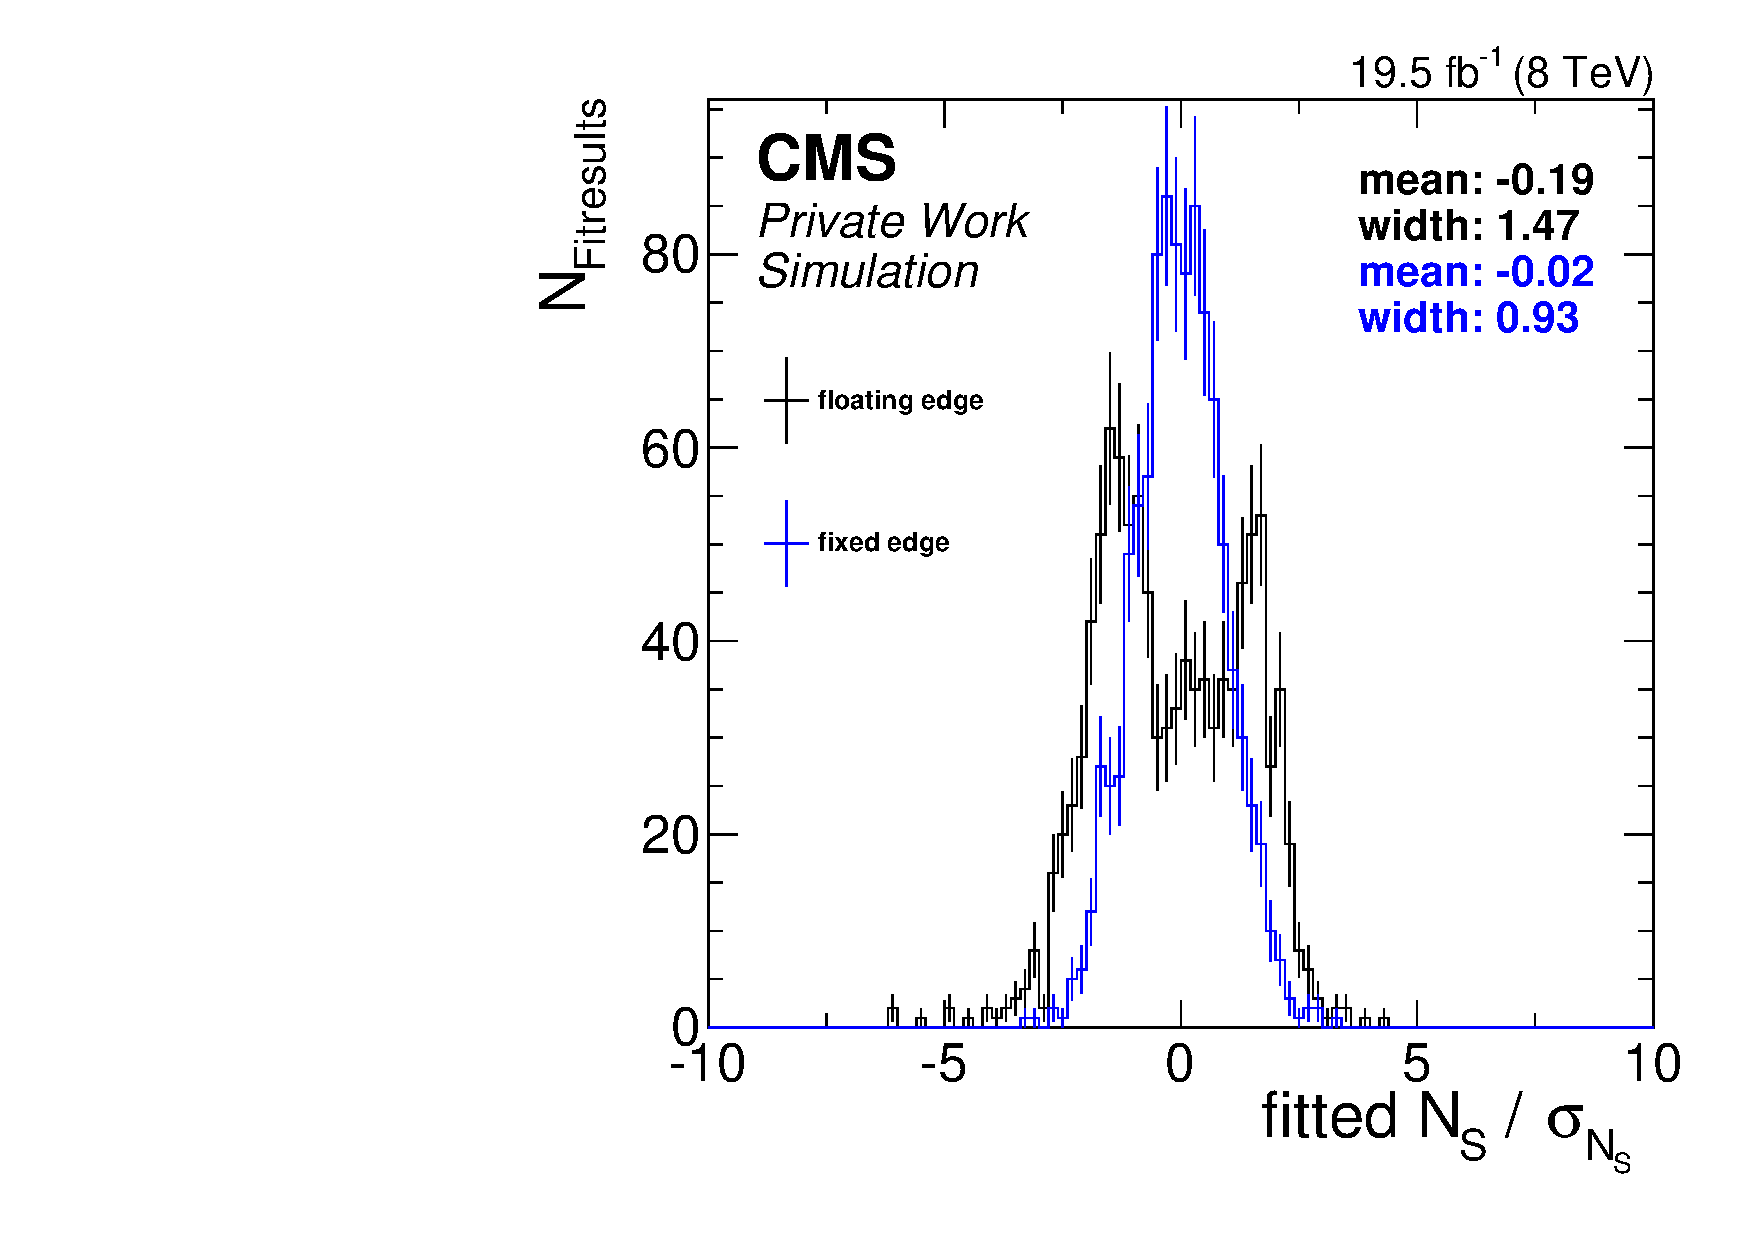
\includegraphics[width=\textwidth]{plots/results/fit/toyResults/nS_floatVsFixed.pdf}
  \end{minipage}
  \begin{minipage}[t]{0.49\textwidth}
    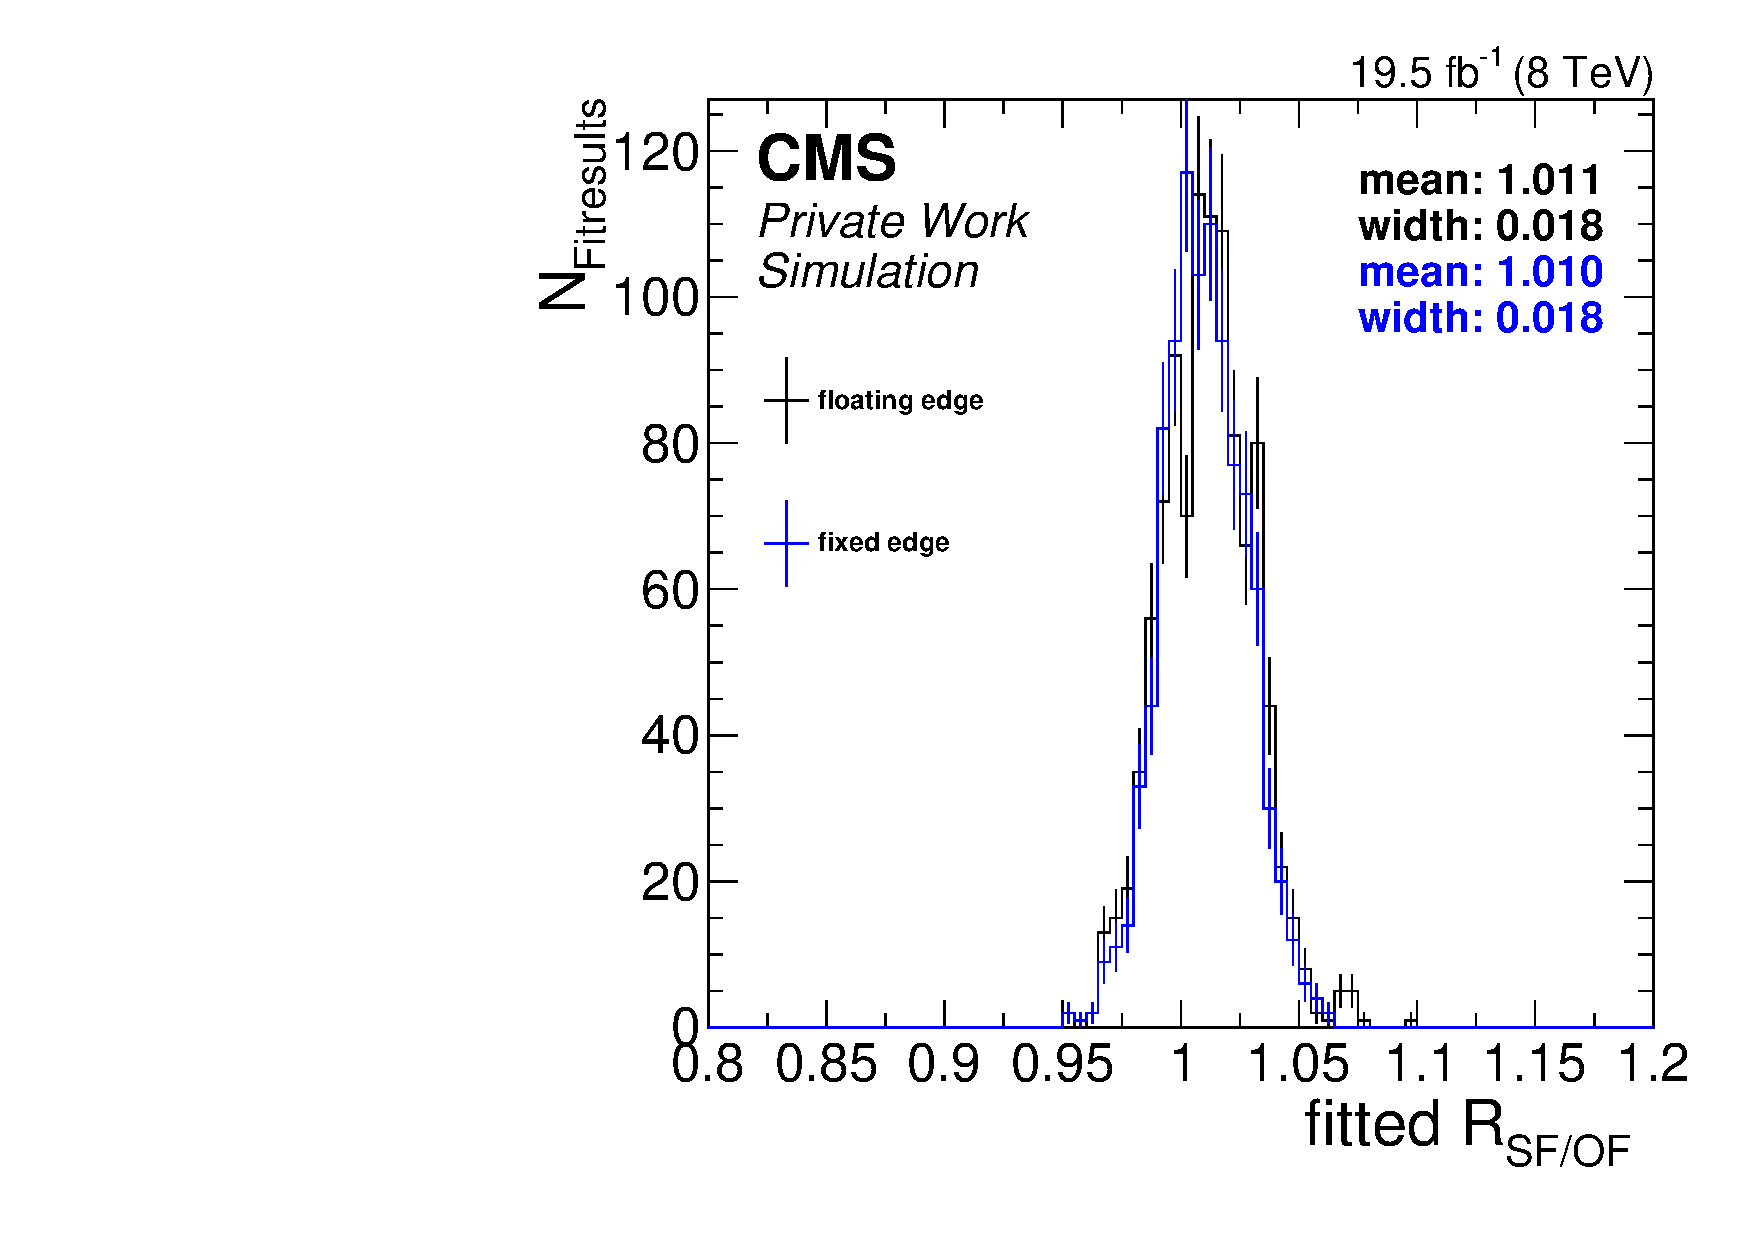
\includegraphics[width=\textwidth]{plots/results/fit/toyResults/rSFOF_floatVsFixed.pdf}
  \end{minipage}

  \caption{Distribution of fit observables in toy studies for a background only scenario. Shown are the fitted number of signal events divided by their uncertainty in the central region (left) and the corresponding fitted values of \Rsfof (right). Shown are results for a floating edge (black) and a fixed edge position (blue).}
  \label{fig:toys:backgroundOnly}
\end{figure}

The distribution of the fitted edge position versus the initial value is shown in Figure~\ref{fig:toys:backgroundOnlyFloatEdge}. The initial values has been randomized between 0 and $\unit{300}{\giga\electronvolt}$. To ensure that the initial value is inside the allowed range for \mlledge, diced values below $\unit{35}{\giga\electronvolt}$ are set to this value. In absence of a signal a strong correlation between the initial and observed value of \mlledge is observed. This suggests that the fit tends to converge to the next local minimum of the negative log-likelihood. It is therefore necessary to choose a suitable initial value close to the global minimum before the fit is performed. 

\begin{figure}[hbp]
  \centering

    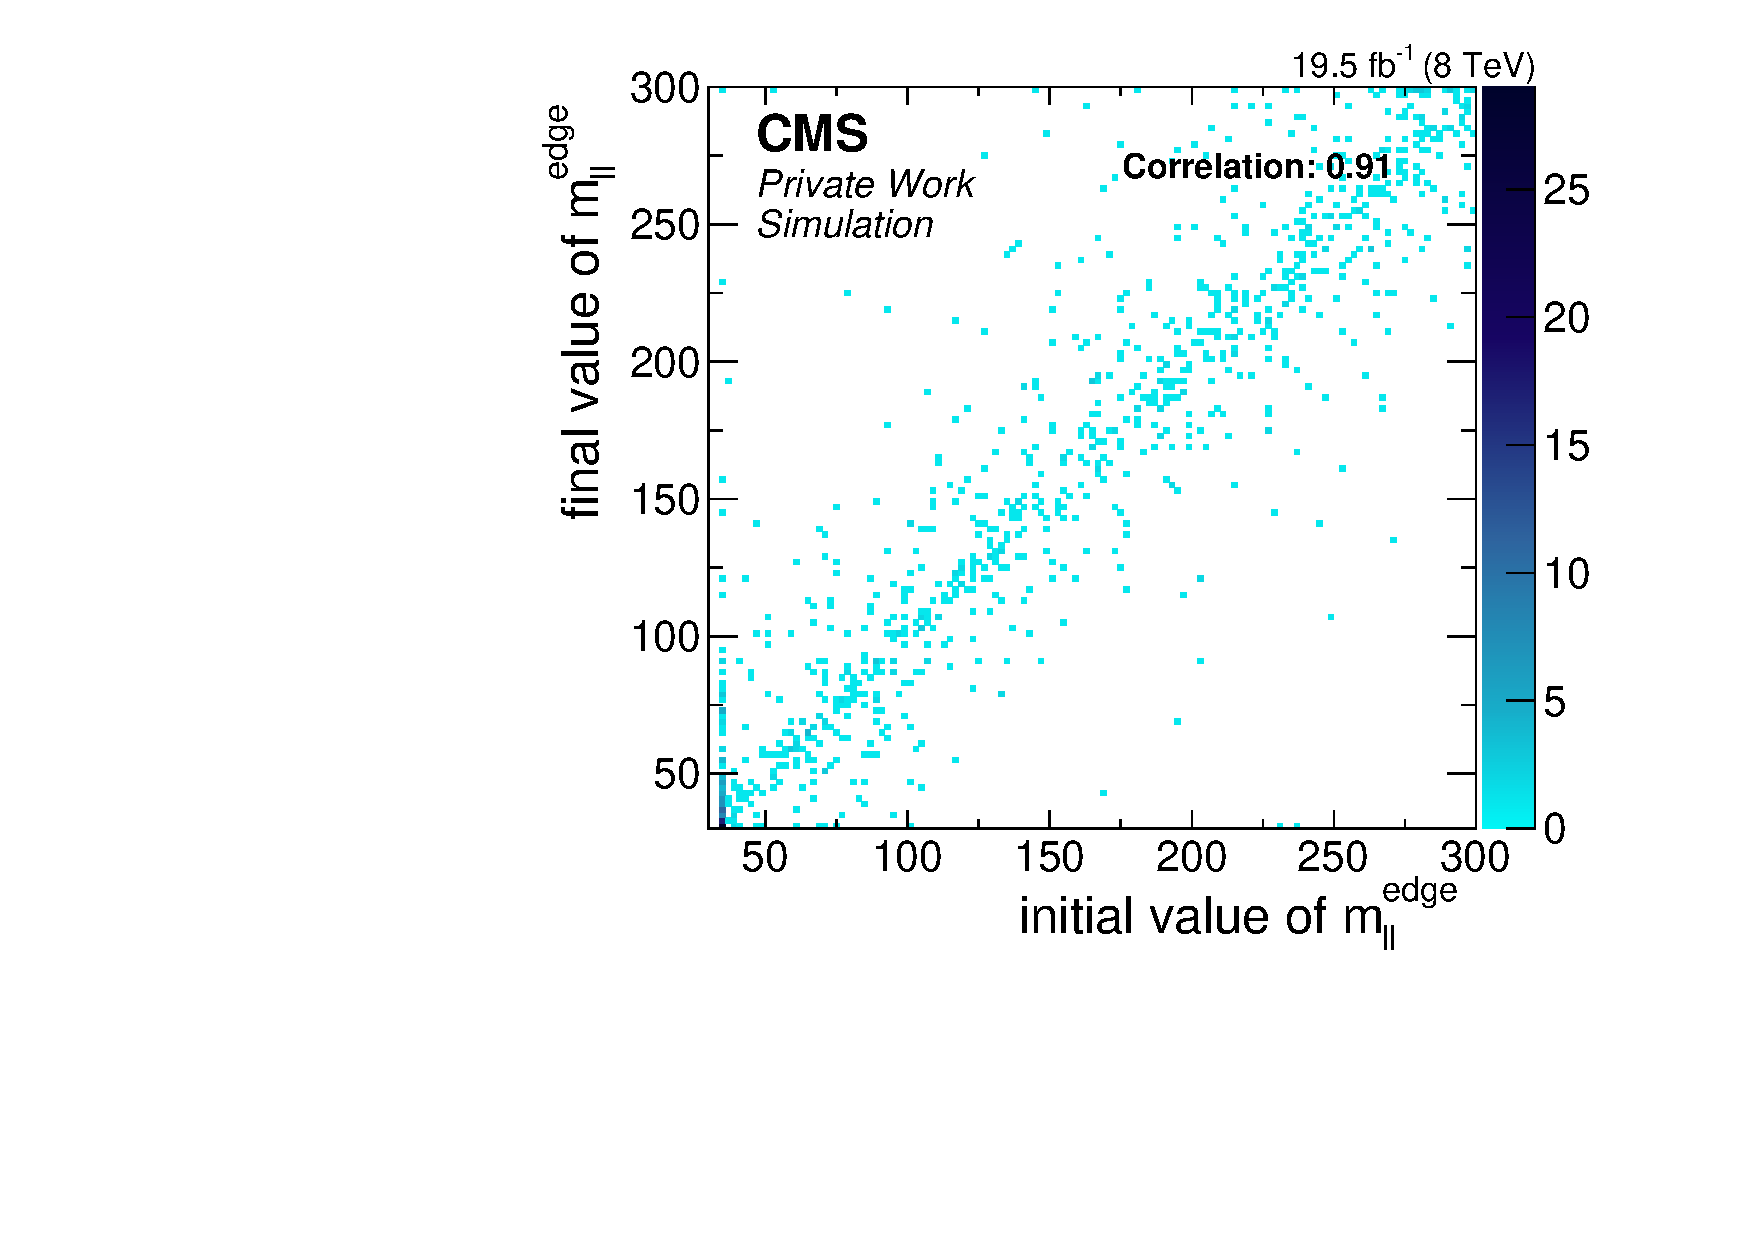
\includegraphics[width=0.6\textwidth]{plots/results/fit/toyResults/fittedM0vsinitialM0_backgroundOnly_randM0_NegSig.pdf}
  \caption{Distribution of fitted versus initial values of \mlledge in the case of the randomized initial values for toys without an injected signal.}
  \label{fig:toys:backgroundOnlyFloatEdge}
\end{figure}

As an additional check, toys are generated with \Rsfof shifted by $\pm1\sigma$. These toys are fitted with the Gaussian constraint to the central value and the results are shown in Figure~\ref{fig:toys:systShift}. The same distributions are shown as above. In the case of the signal yield divided by its uncertainty, the double peak structure observed in the nominal configuration changes to a single peak that is shifted to negative signal yields for the toys generated with lower and to positive signal yields for those generated with higher values of \Rsfof. For the fitted values of \Rsfof, the width of the distribution is unchanged, but the systematic shifts in the generation of the toys is reflected in their means. However, the observed shifts of the mean (0.025 and -0.023) are smaller than those introduced the generation of the toys ($\pm0.037$, the uncertainty of \Rsfof), suggesting that part of the systematic shift is absorbed by the fit by introducing a signal contribution.
\begin{figure}[!hbp]
  \centering
  \begin{minipage}[t]{0.49\textwidth}
    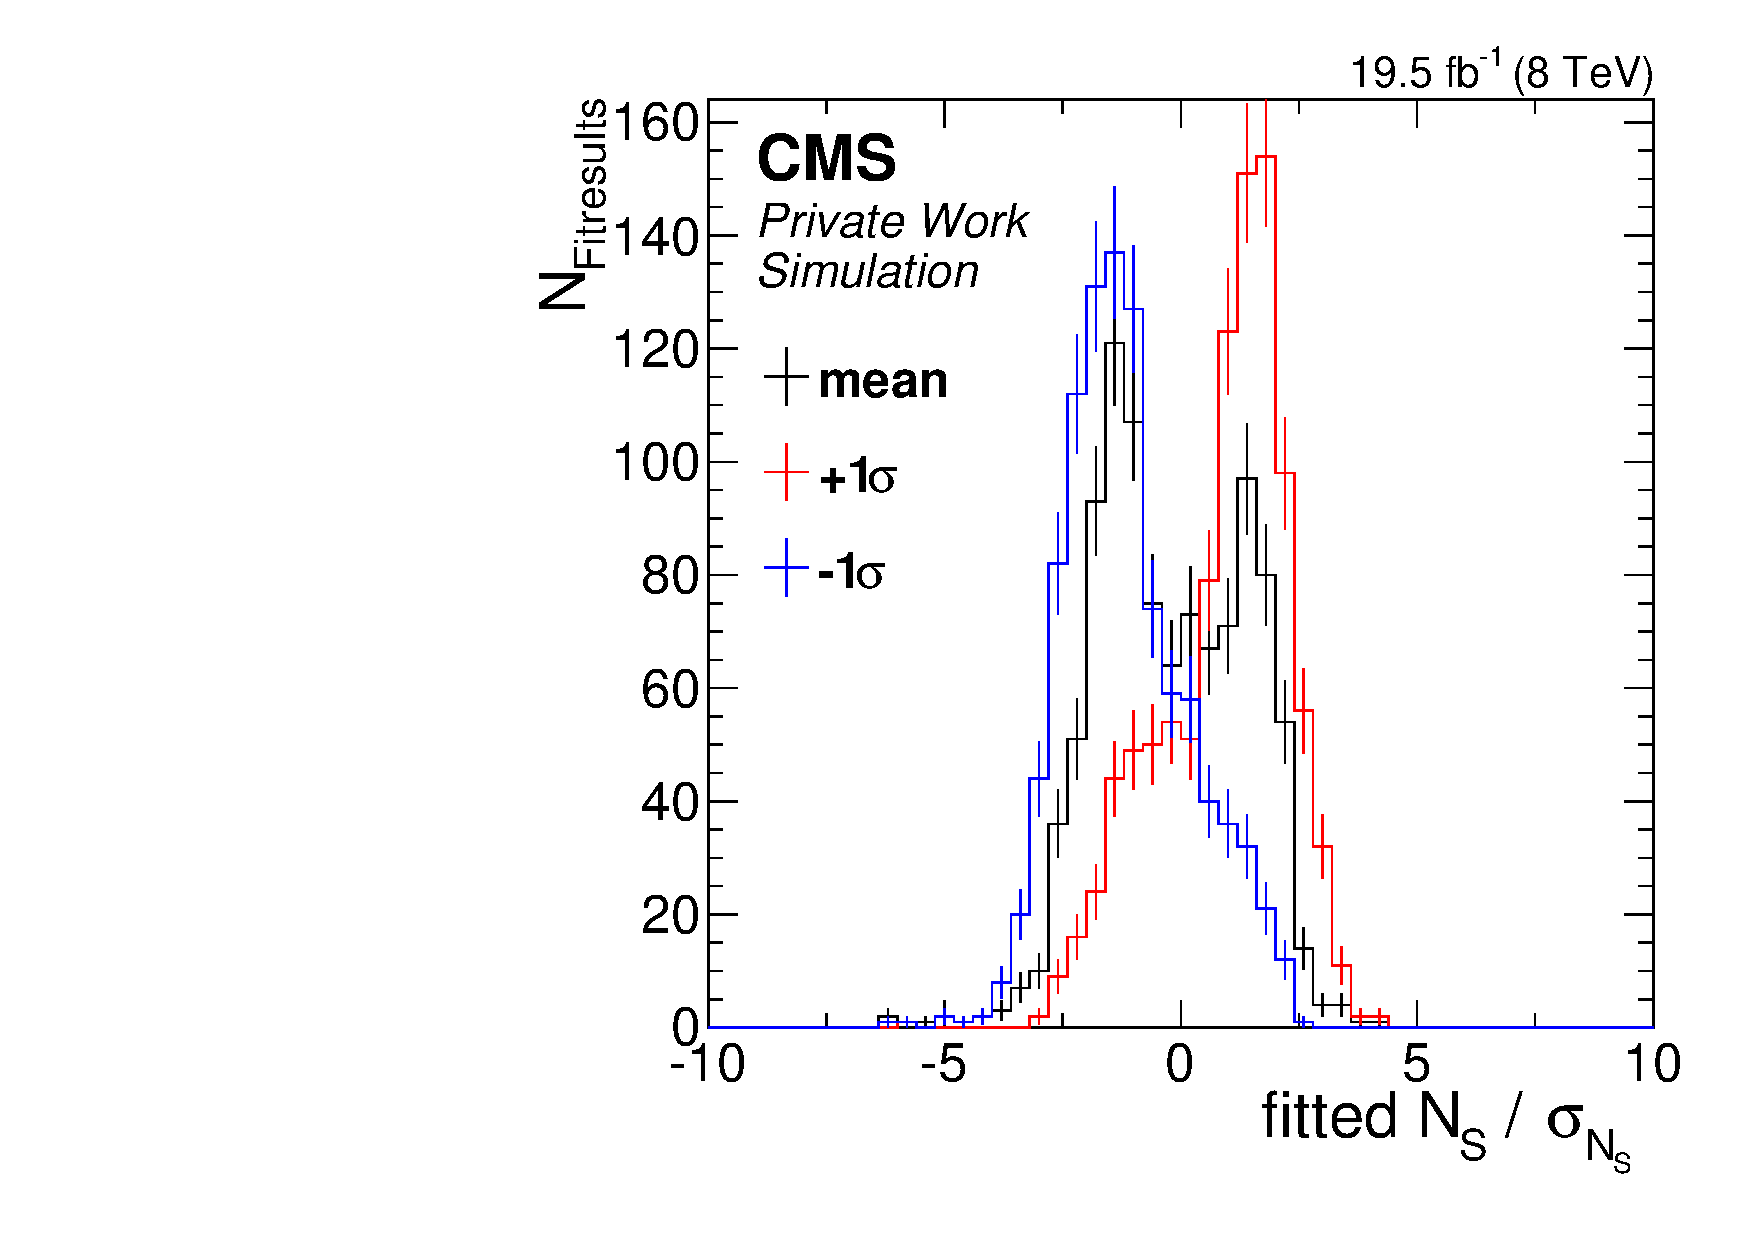
\includegraphics[width=\textwidth]{plots/results/fit/toyResults/nS_systShift.pdf}
  \end{minipage}
  \begin{minipage}[t]{0.49\textwidth}
    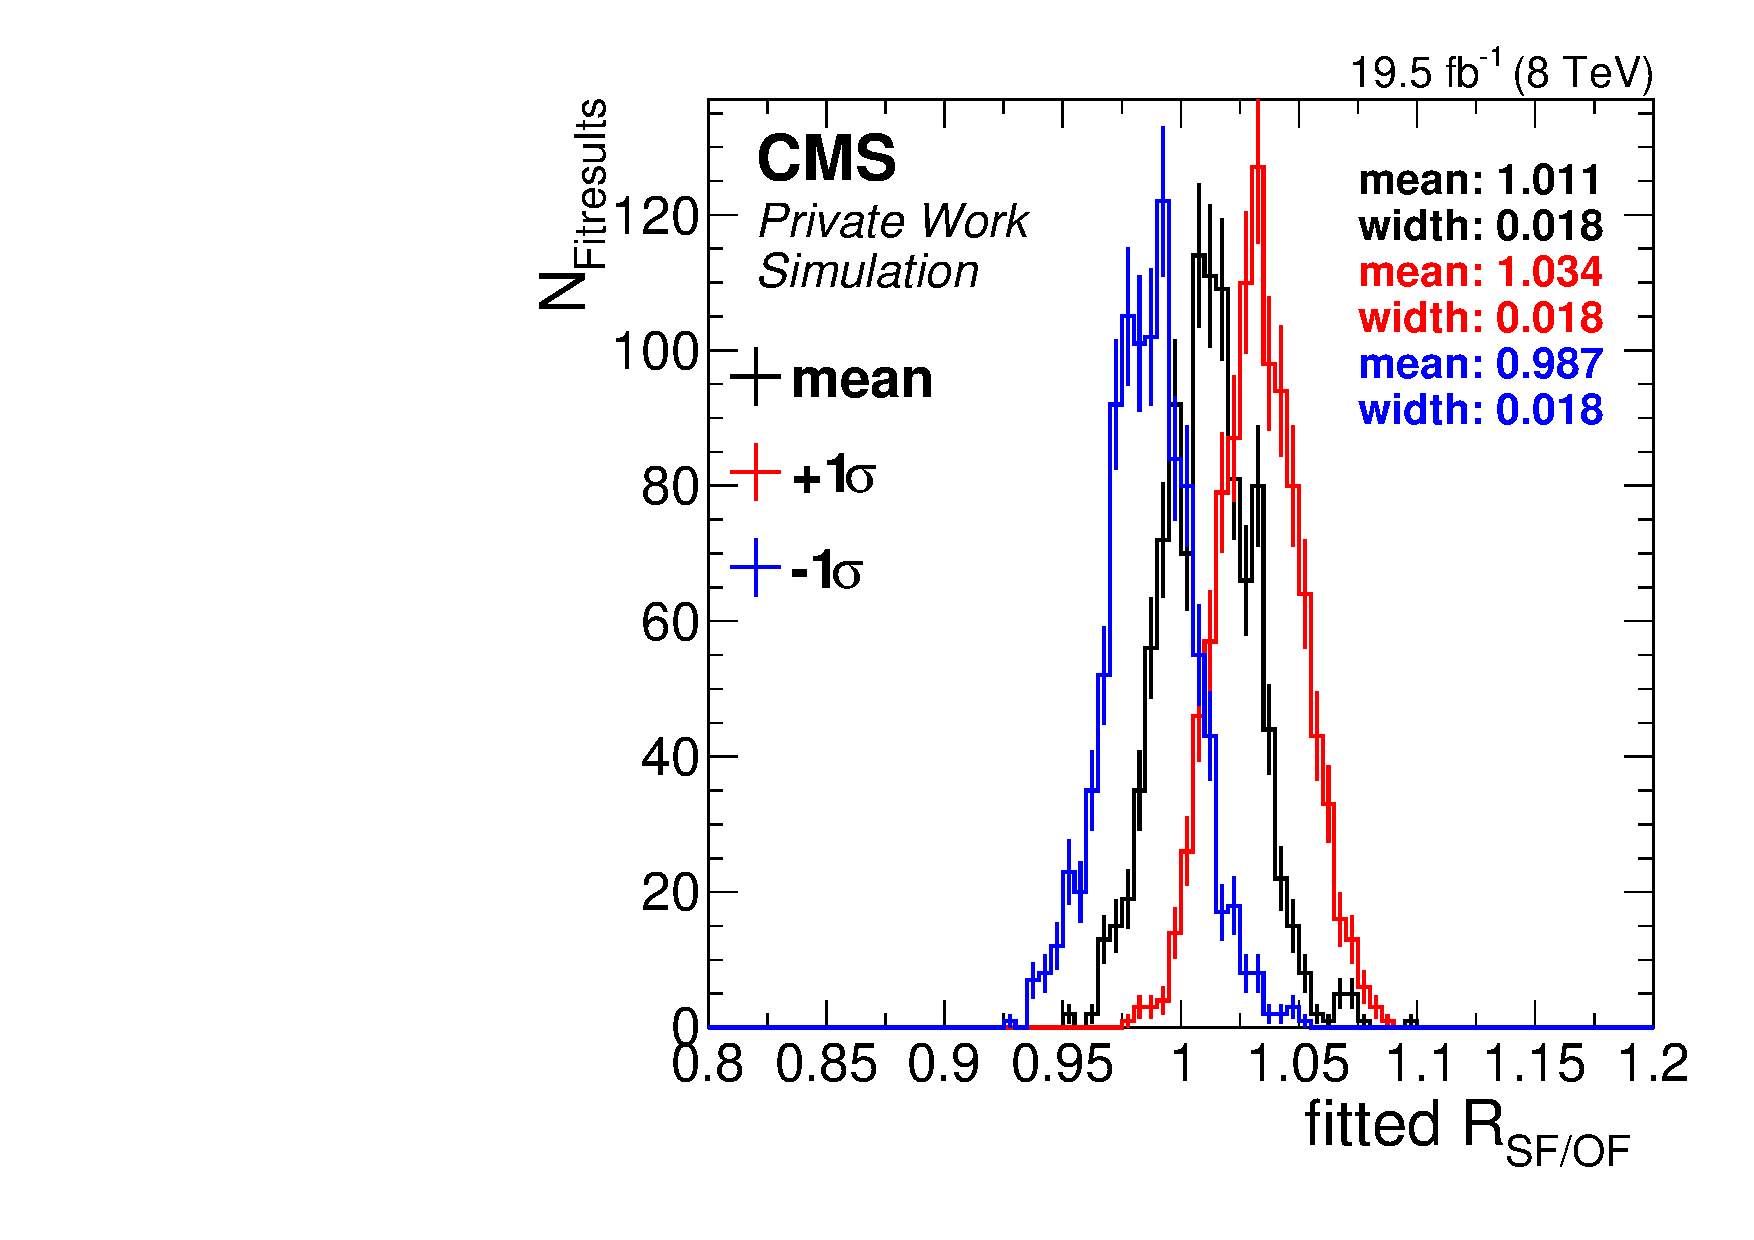
\includegraphics[width=\textwidth]{plots/results/fit/toyResults/rSFOF_systShift.pdf}
  \end{minipage}

  \caption{Distribution of fit observables in toy studies for background only toys with fixed edge position. Shown are the fitted number of signal events in the central region (left) and the fitted number of signal events divided by the fitted uncertainty in the central region (right).}
  \label{fig:toys:systShift}
\end{figure}
\newpage
\subsubsection{Toy studies with signal injection}
The fit performance in the presence of a signal is tested by injection a signal of 125 events with and edge position of 70 GeV in the central region and again a third of that number in the forward signal region. Figure \ref{fig:toys:signalInjected} shows the resulting distribution of fit results for a selection of observables in the central signal region. The distribution of the number of signal events is well described by a Gaussian with a mean of about 126 events, very close to the injected number, and a width of 41 events. Divided by the fitted uncertainty this gives a unit Gaussian with a mean of about 2.9. The edge position is also Gaussian distributed, with a mean of about $\unit{70}{\giga\electronvolt}$, also reproducing the injected value very well, with a width of about $\unit{1.8}{\giga\electronvolt}$. Comparing the distribution of \Rsfof with that in Figure~\ref{fig:toys:backgroundOnly}, it can be seen that the presence of a signal does not bias the result towards higher values. 

\begin{figure}[hbp]
  \centering
  \begin{minipage}[t]{0.49\textwidth}
    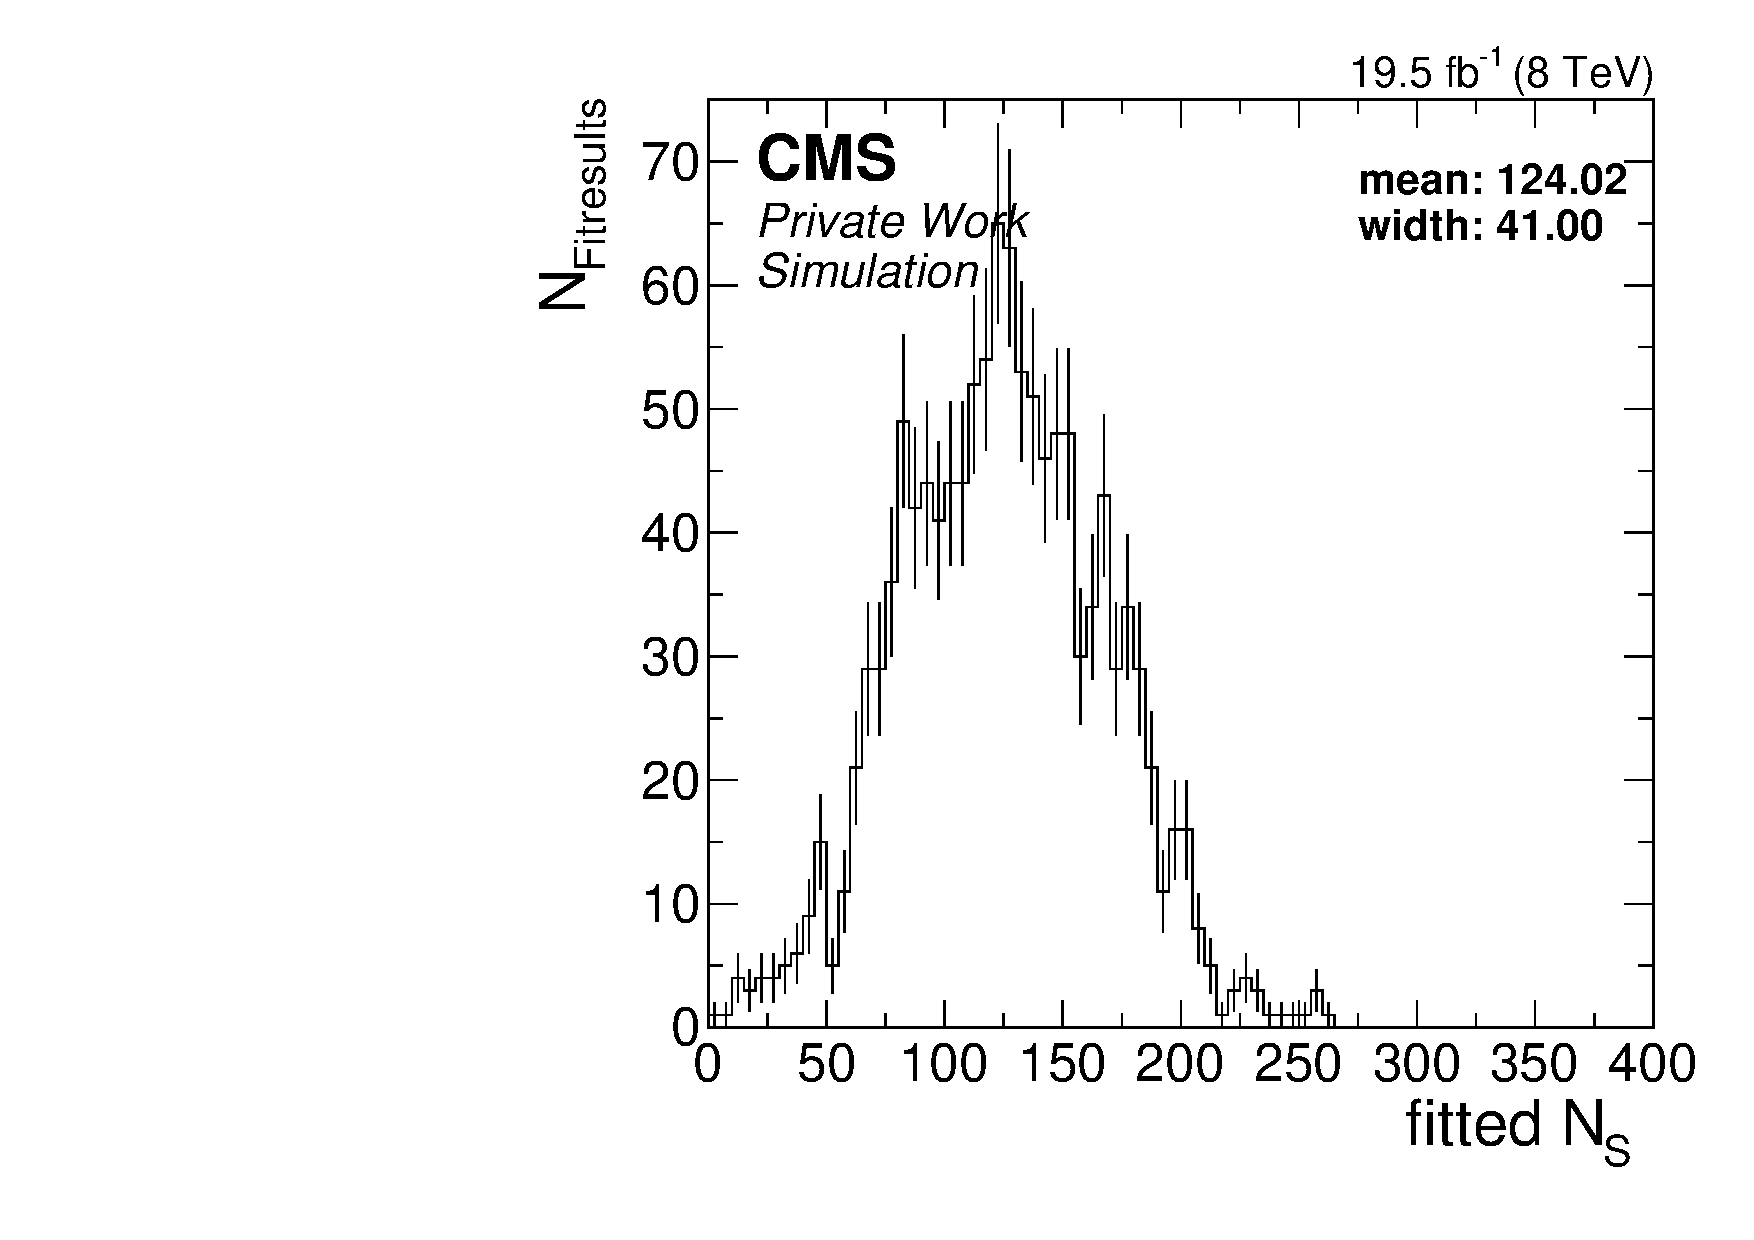
\includegraphics[width=\textwidth]{plots/results/fit/toyResults/nSPure_signalInjected.pdf}
  \end{minipage}
  \begin{minipage}[t]{0.49\textwidth}
    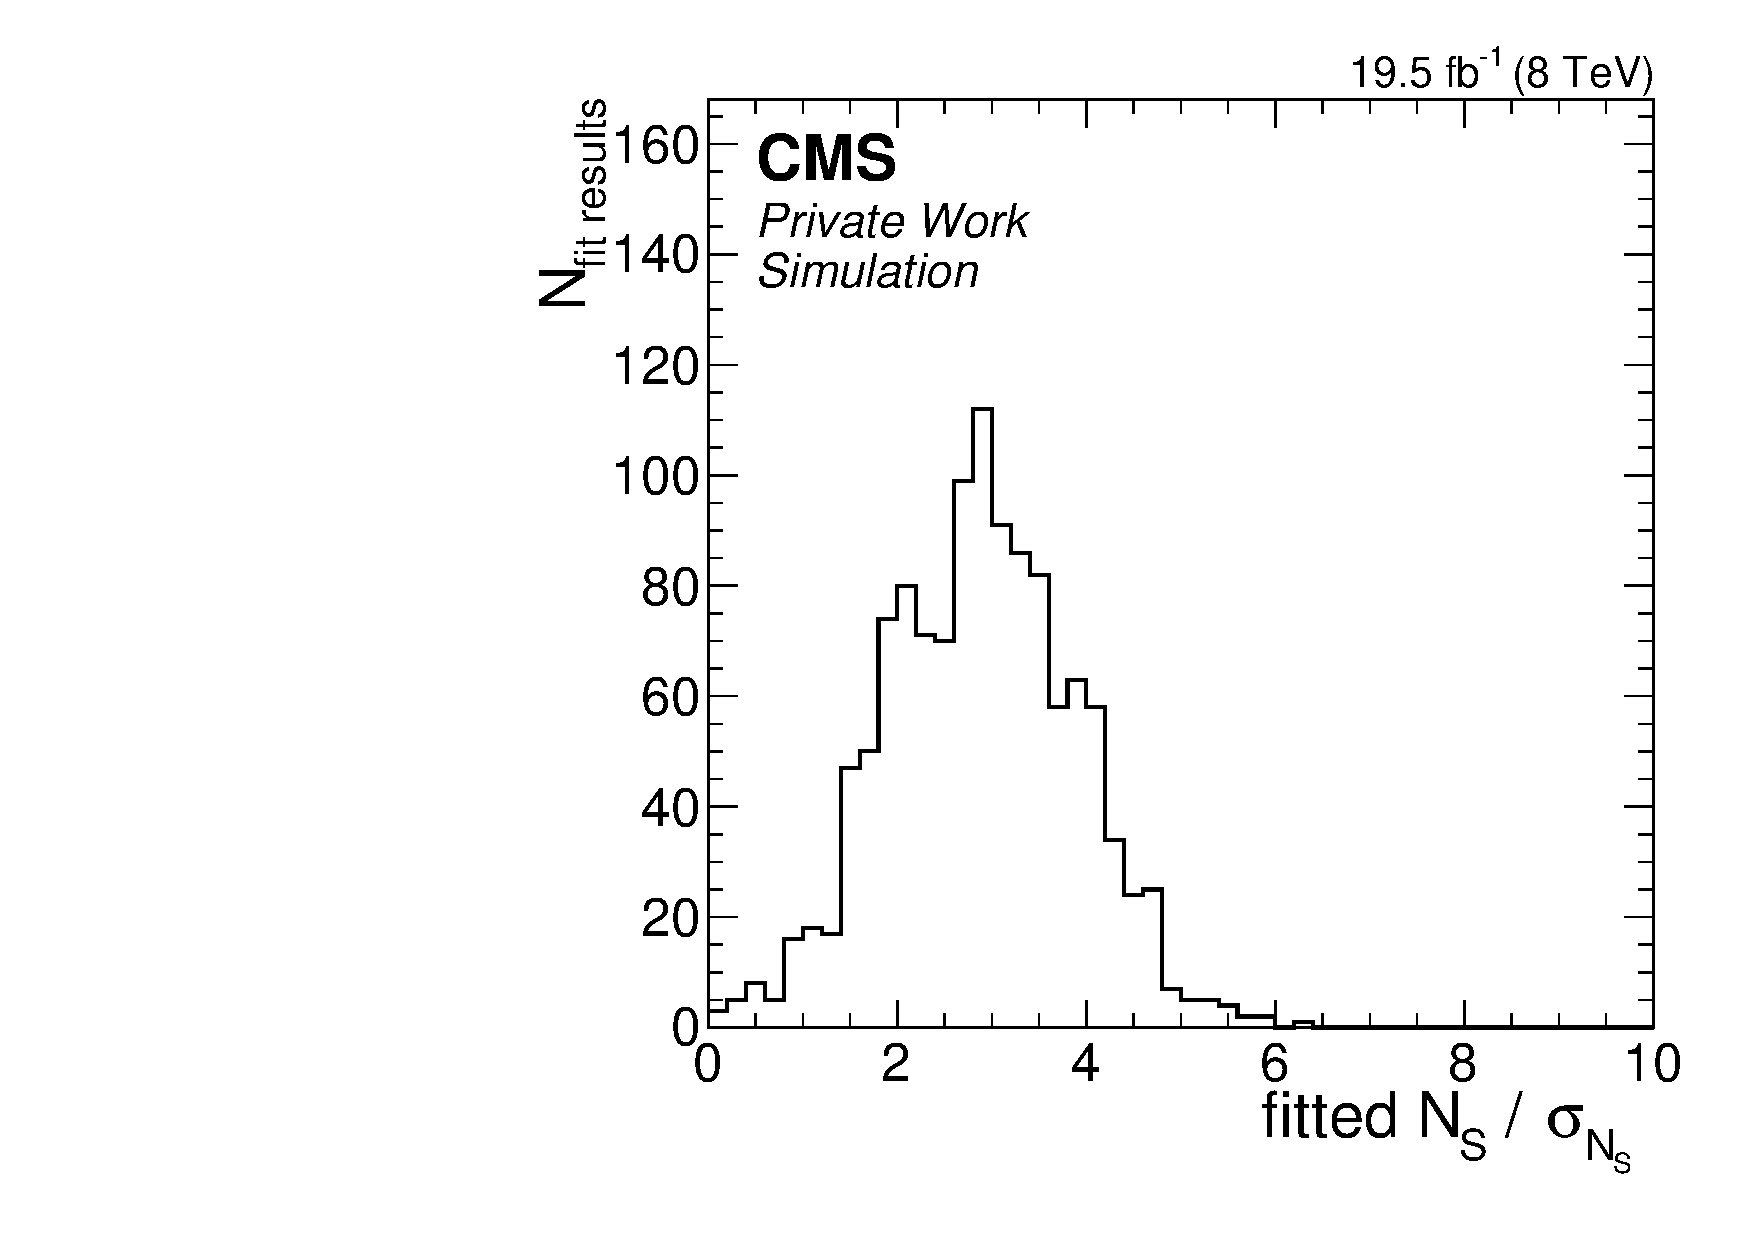
\includegraphics[width=\textwidth]{plots/results/fit/toyResults/nS_signalInjected.pdf}
  \end{minipage}
  \begin{minipage}[t]{0.49\textwidth}
    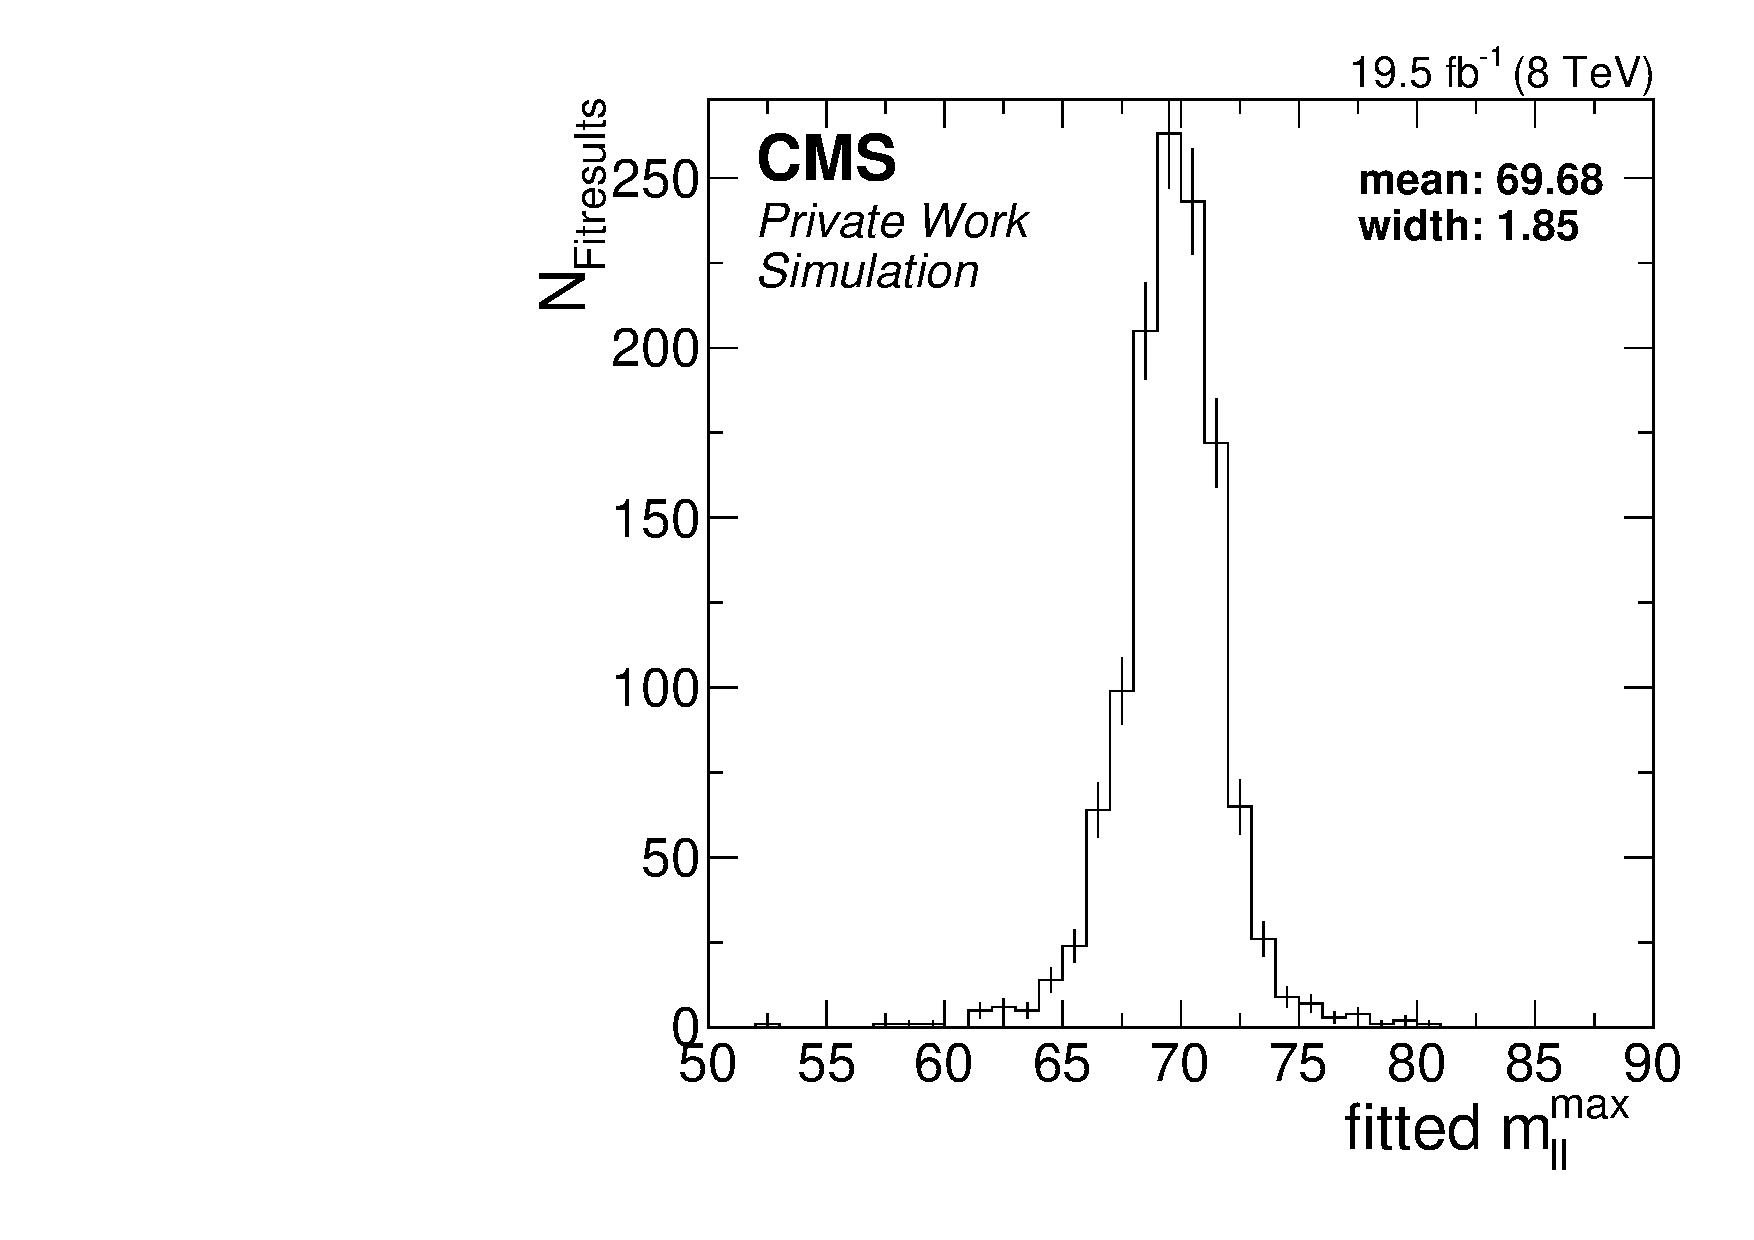
\includegraphics[width=\textwidth]{plots/results/fit/toyResults/m0_signalInjected.pdf}
  \end{minipage}
  \begin{minipage}[t]{0.49\textwidth}
    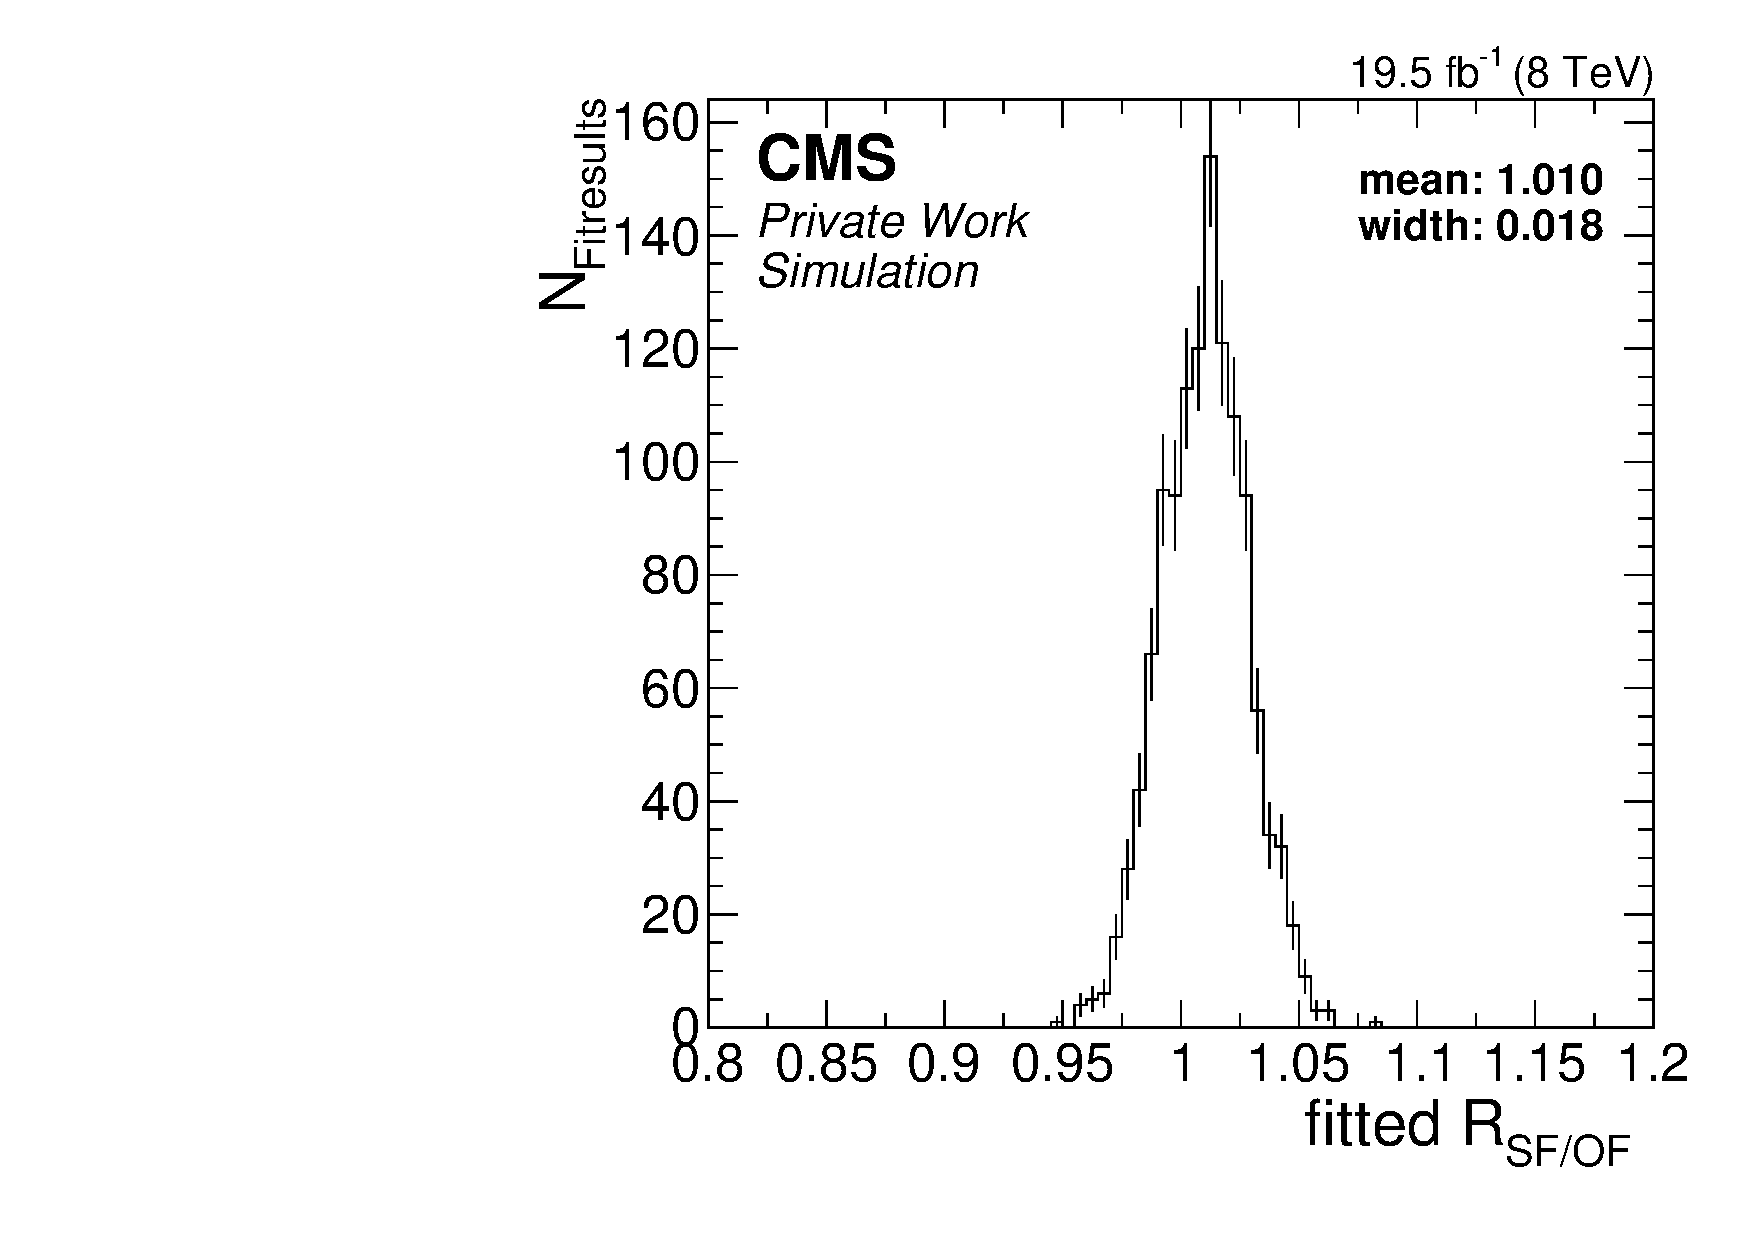
\includegraphics[width=\textwidth]{plots/results/fit/toyResults/rSFOF_signalInjected.pdf}
  \end{minipage}
  \caption{Distribution of fit observables in toy studies with a signal injected. Shown are the fitted number of signal events in the central region (upper left), the fitted number of signal events divided by the fitted uncertainty in the central region (upper right), the fitted edge position (lower left) and the fitted \Rsfof in the central region (lower right).}
  \label{fig:toys:signalInjected}
\end{figure}

To study the dependence of the fit result on the edge position, toys are generated with a signal of 125 events in the central signal region injected for different values of \mlledge between 40 and 200\GeV in steps of 10\GeV. For each configuration, about 1000 fits are performed. The initial value of \mlledge is chosen to coincide with the generated one. The distributions of the fitted \mlledge and number of signal events for each generated \mlledge are shown in Figure~\ref{fig:toys:scan}. In the case of the fitted \mlledge on the left side, the generated value is in general very well reproduced by the fit. The best results are obtained for low values of \mlledge, as the signal shape is much steeper and easier to separate from the background as for higher values. Towards higher values the spread of the results and especially the probability for very large deviation from the generated value increases, before they decrease slightly towards very high values of the generated \mlledge. A notable feature is observed for generated values of 100\GeV, where for a small number of fits the fitted value is very close to the Z boson mass. Similar behaviour is also observed for the number of fitted signal events. Here the relative size of the deviation form the generated value is much larger, as the event yields are fluctuated in the generation of the toys. 
\begin{figure}[!hbp]
  \centering
  \begin{minipage}[t]{0.49\textwidth}
    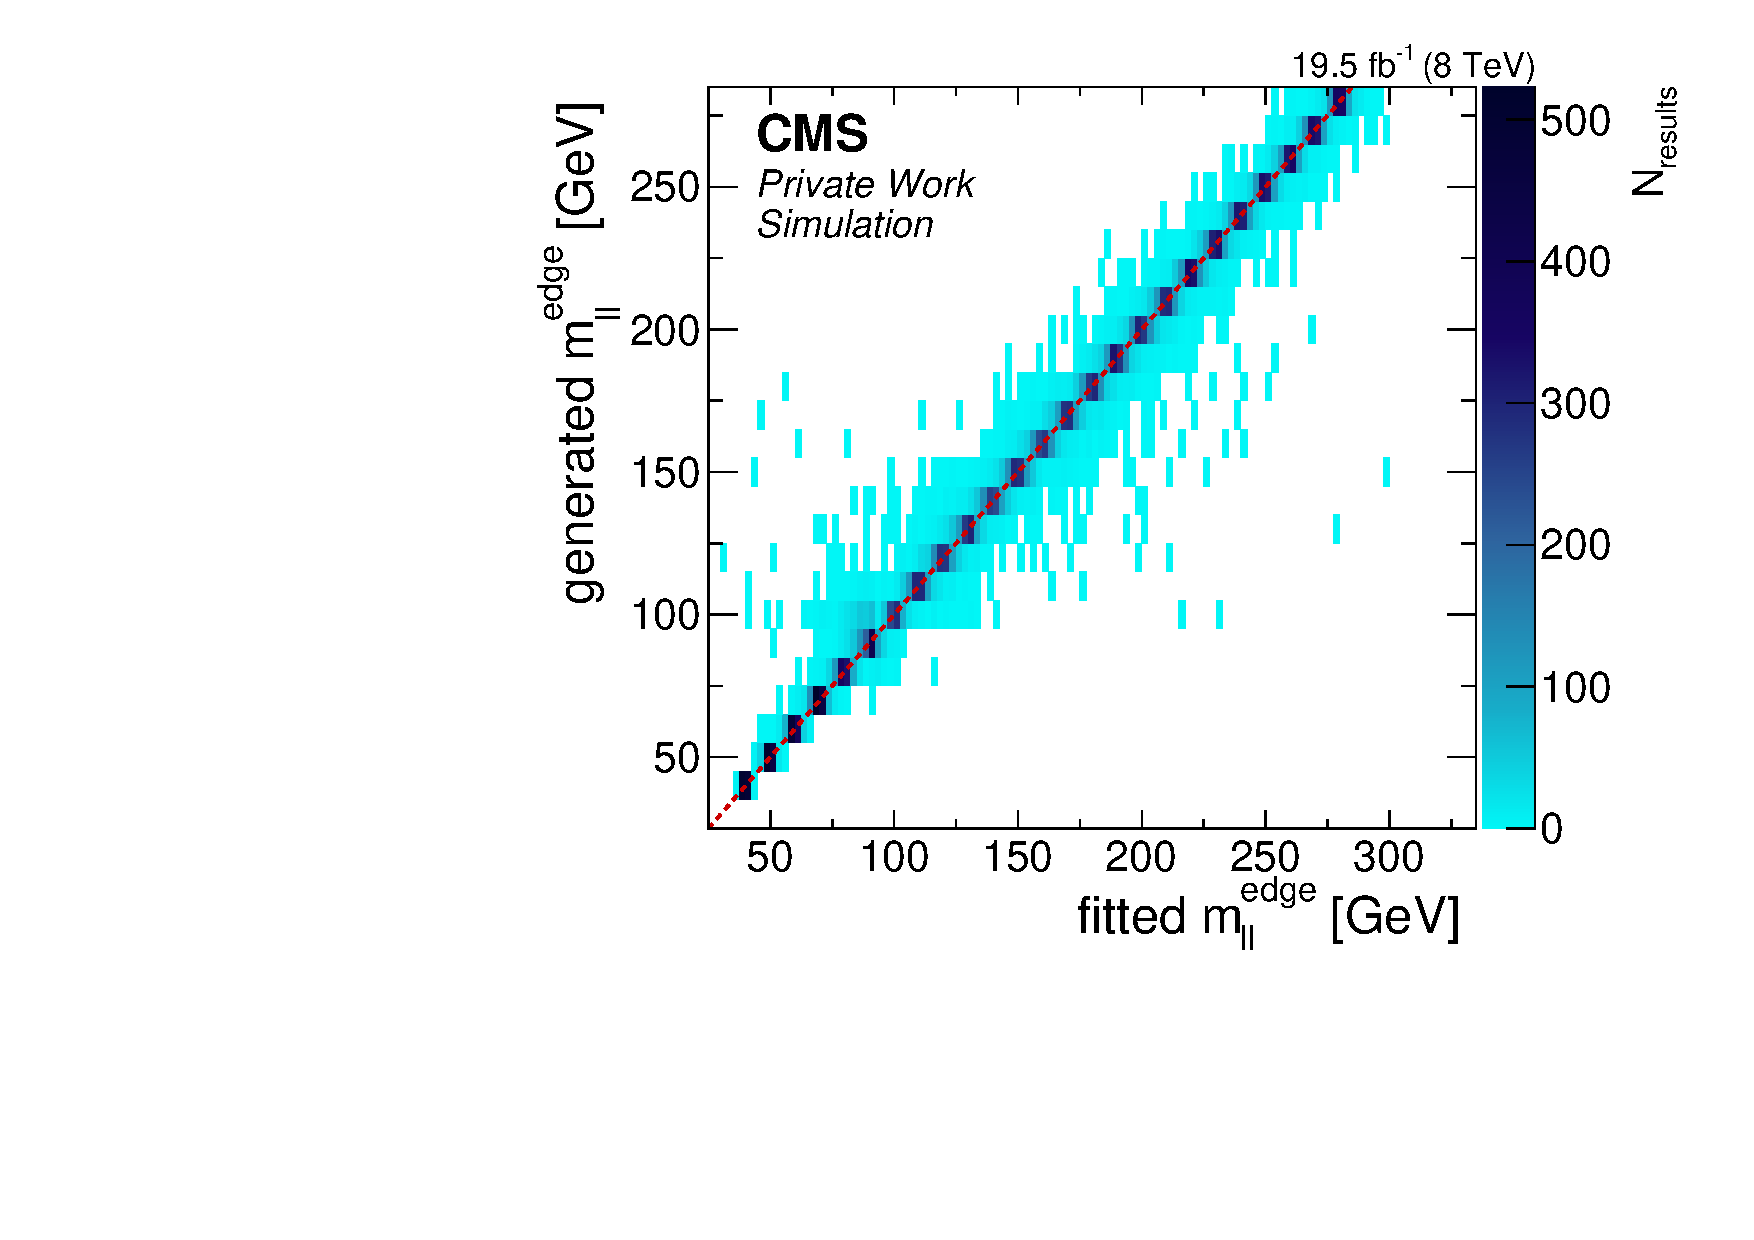
\includegraphics[width=\textwidth]{plots/results/fit/toyResults/generatedM0vsfittedM0_signalInjectedN125.pdf}
  \end{minipage}
  \begin{minipage}[t]{0.49\textwidth}
    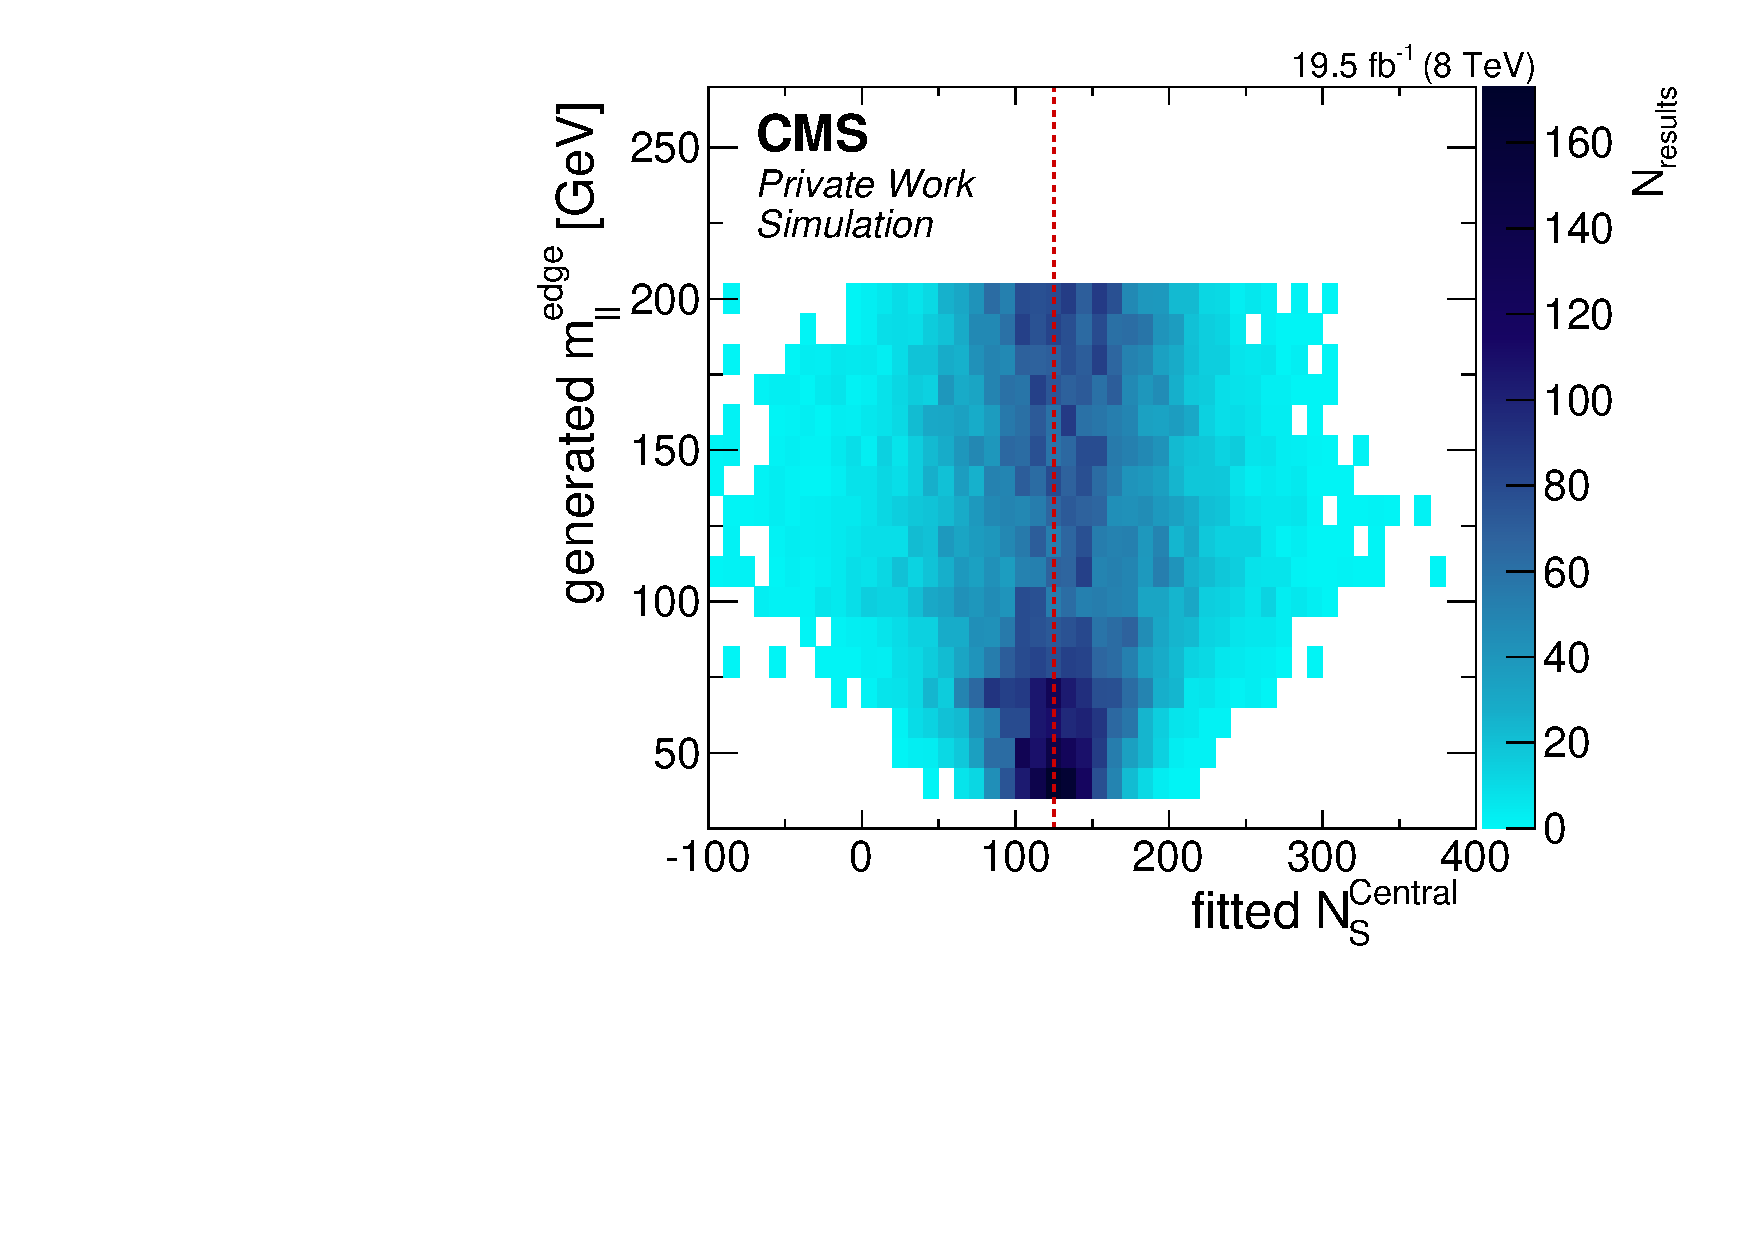
\includegraphics[width=\textwidth]{plots/results/fit/toyResults/generatedM0vsfittedNS_signalInjectedN125.pdf}
  \end{minipage}
  \caption{Distributions of the fitted \mlledge (left) and the number of signal events (right) for each generated \mlledge. The frequency of the results is colour-coded, darker colours indicating higher values. The dashed red lines indicate the points at which the fitted result matches the generated value.}
    \label{fig:toys:scan}
\end{figure}

The width of the distribution of the fitted \mlledge is shown on the left side of Figure~\ref{fig:toys:scanFits}. It is quantified both with the root mean square (RMS) of the distribution and the width of a Gaussian fitted in a range of $\pm\unit{3}{\giga\electronvolt}$ around the generated value. The first is sensitive to the non-Gaussian tails of the distribution while the latter is a measure of the core resolution. For generated values of \mlledge of $\unit{40}{\giga\electronvolt}$, the two values are the same, but quickly deviate for higher edge positions. The Gaussian width rises from about $\unit{1}{\giga\electronvolt}$ to about $\unit{2-2.5}{\giga\electronvolt}$ for edge position above $\unit{80}{\giga\electronvolt}$ and is roughly constant for higher edge positions. The RMS reaches values of $\unit{4}{\giga\electronvolt}$ for edges below the Z mass. For $\unit{\mlledge=100}{\giga\electronvolt}$ it is much larger, caused by the bias towards the Z mass observed in Figure~\ref{fig:toys:scan}. Above the Z peak the RMS of the distribution is stable at $\unit{8}{\giga\electronvolt}$ before it drops off again at very high edge positions.

The right side of Figure~\ref{fig:toys:scanFits} shows the means and widths of fits of Gaussian functions to the distributions of $N_{S}^{central}$, again as a function of the generated \mlledge. The distributions do not exhibit significant non-Gaussian tails, so the RMS value is not shown in this case. The injected value of 125 events reproduced within about 8 events for all values of \mlledge. The width increases with \mlledge from roughly 25 to 65 events at \mlledge of $\unit{100}{\giga\electronvolt}$ and decreases slightly for higher values.

\begin{figure}[!hbp]
  \centering
  \begin{minipage}[t]{0.49\textwidth}
    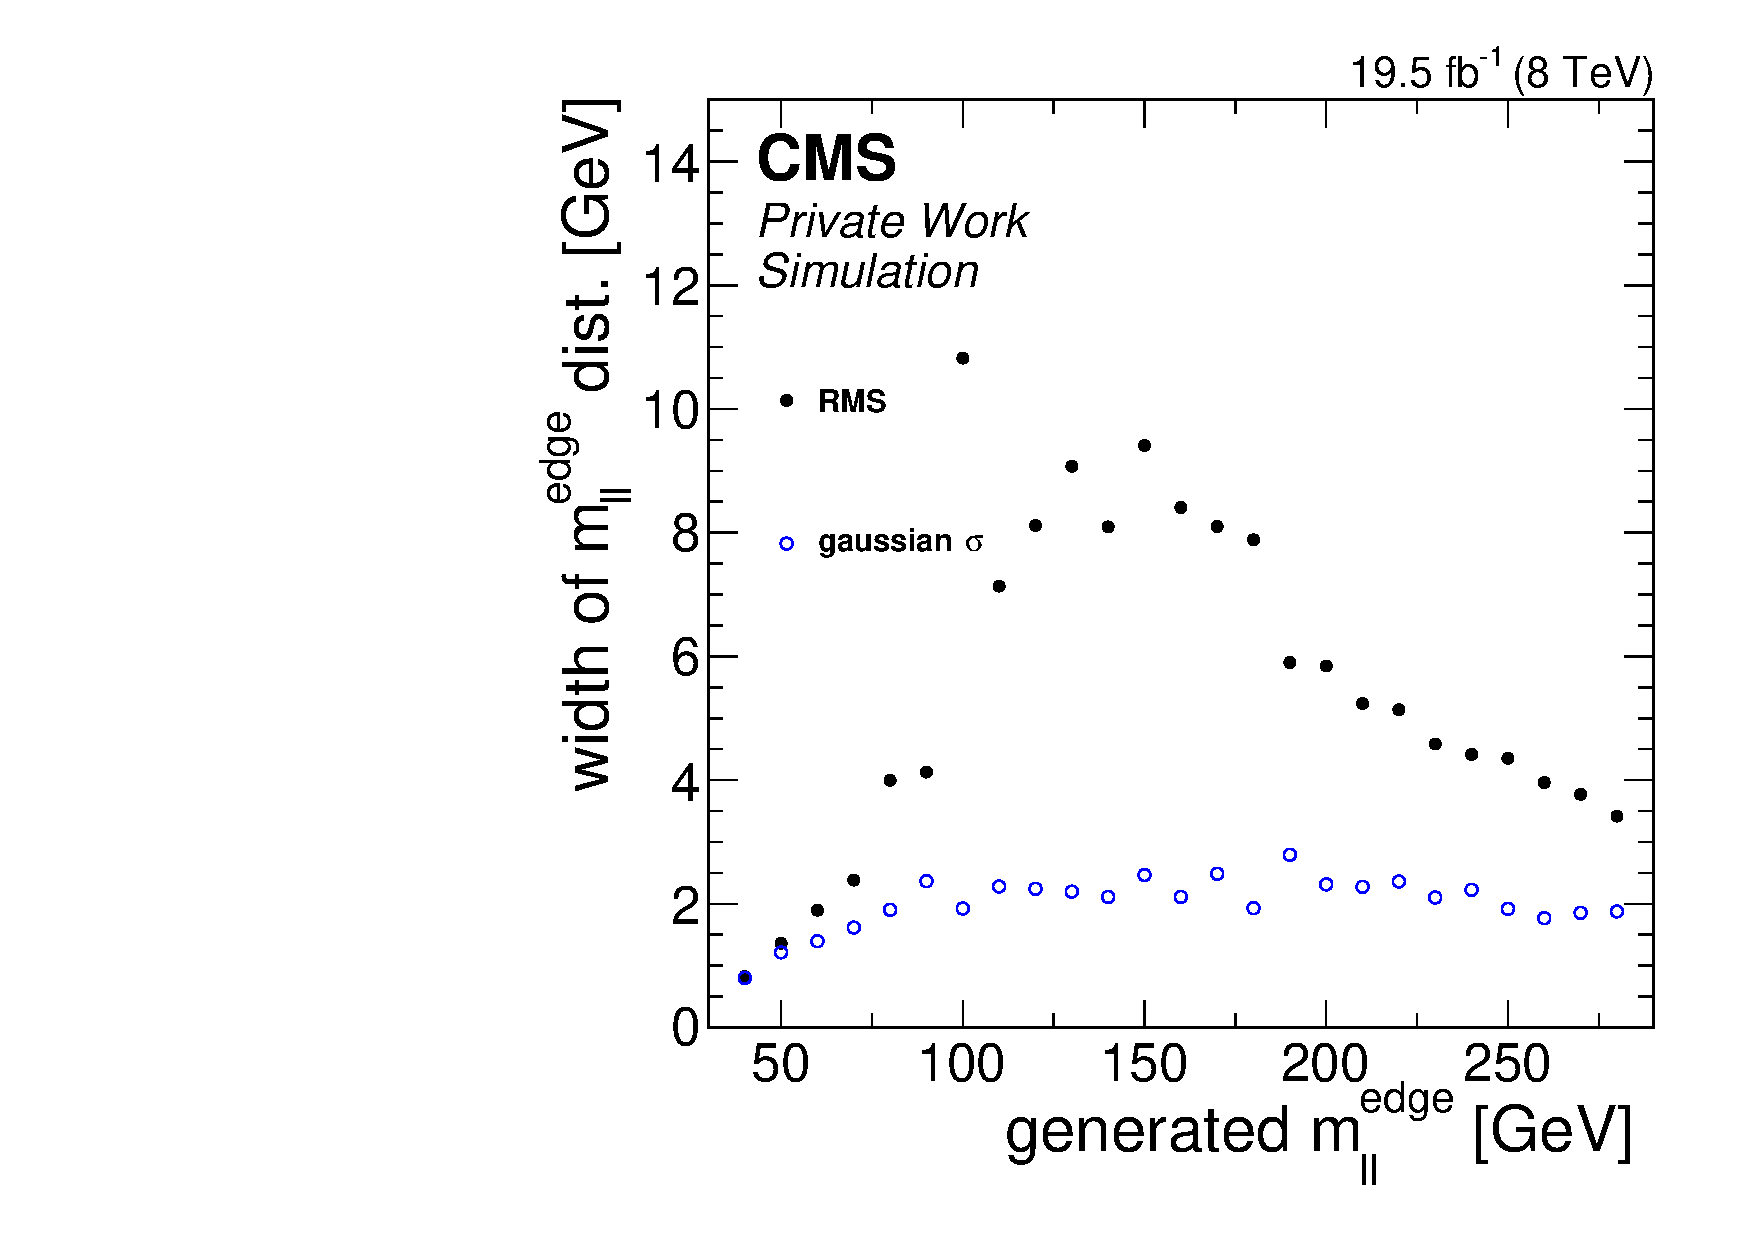
\includegraphics[width=\textwidth]{plots/results/fit/toyResults/WidthsvsGenM0Ratio_signalInjectedN125.pdf}
  \end{minipage}
  \begin{minipage}[t]{0.49\textwidth}
    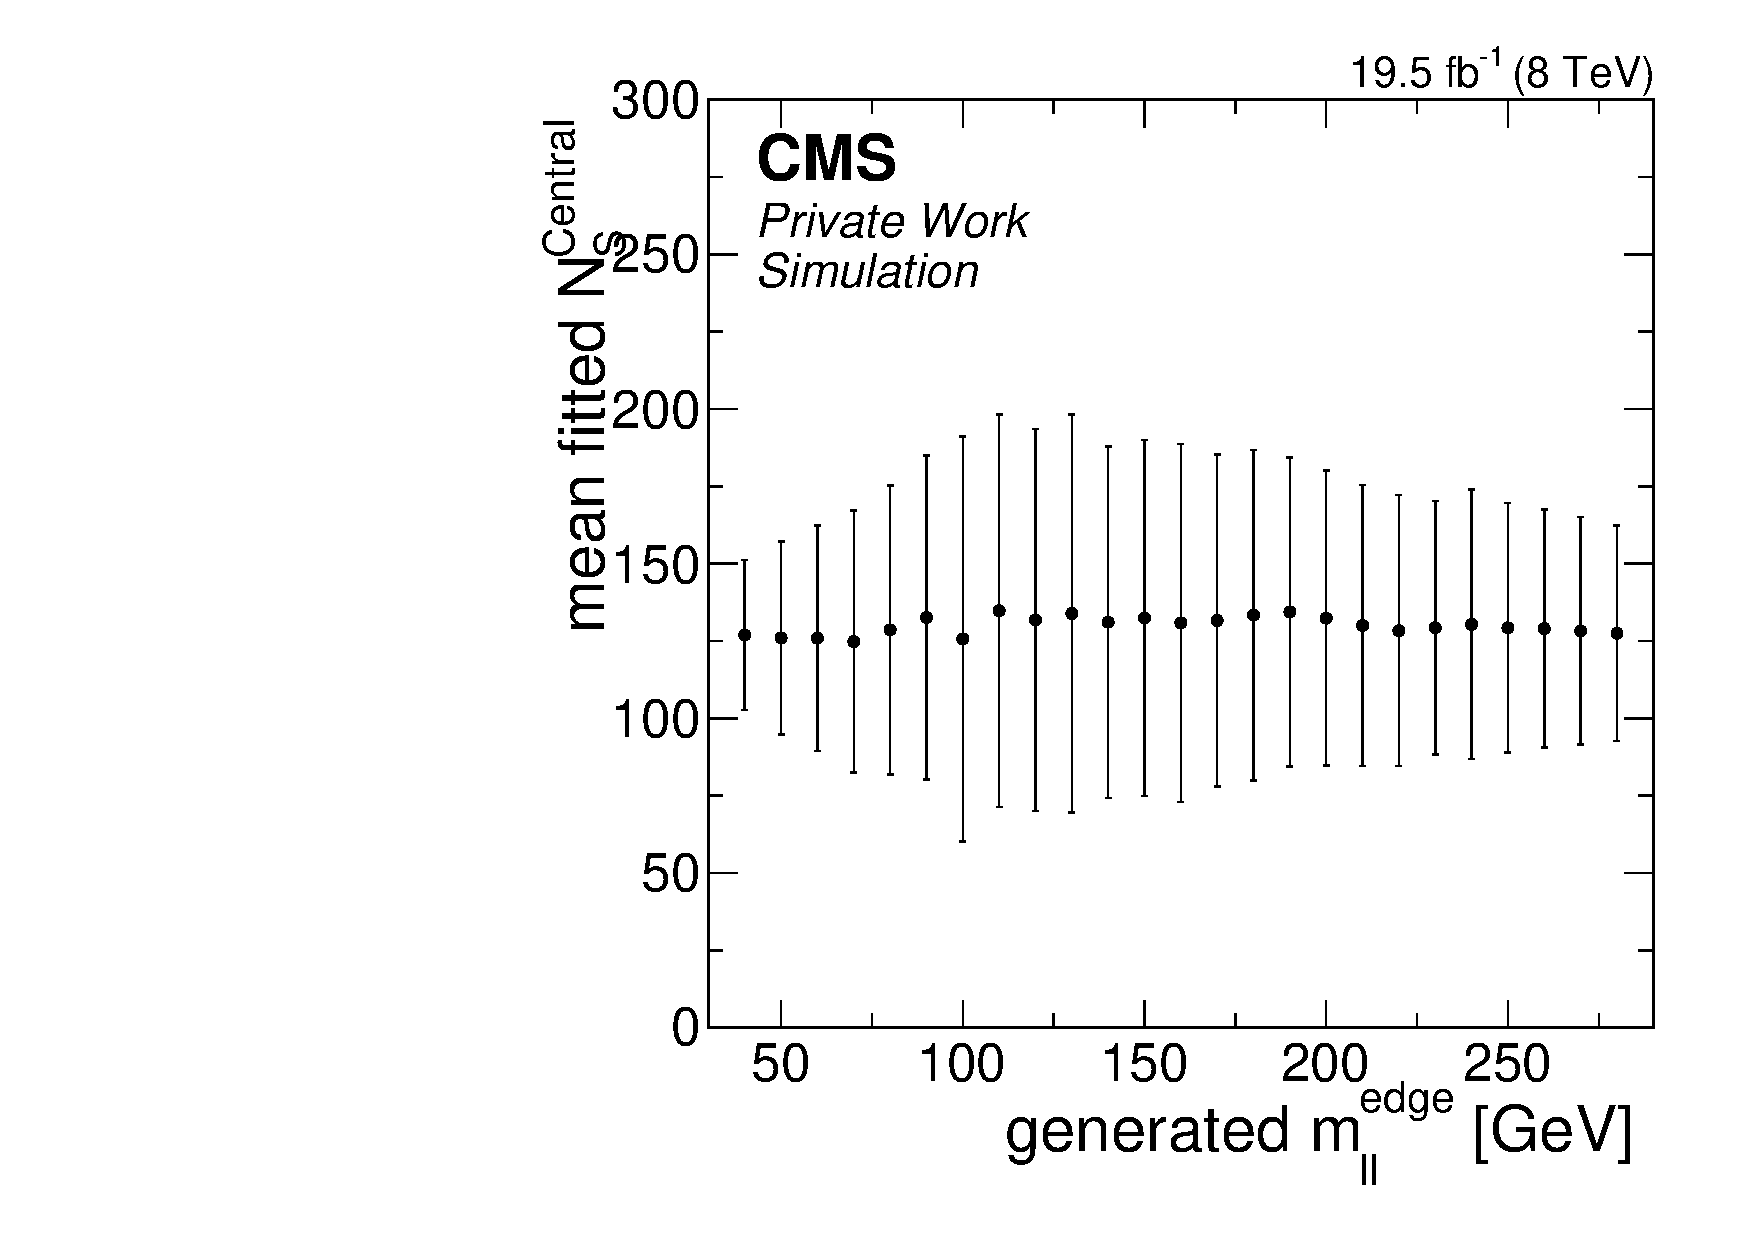
\includegraphics[width=\textwidth]{plots/results/fit/toyResults/meanNSvsGenM0_signalInjectedN125.pdf}
  \end{minipage}
  \caption{Fitted idths of the \mlledge (left) and means and widths $N_S^{central}$ distributions (right) as a function of the generated \mlledge.}
    \label{fig:toys:scanFits}
\end{figure}

To test deviations from the assumed signal shape, toys are generated with and signal injected at $\unit{\mlledge = 70}{\giga\electronvolt}$ and a size of 125 events, but following the convex and concave signal shapes described in section~\ref{sec:sigModel}. They are then fitted using the nominal triangular signal shape. Resulting distributions are shown in Figure~\ref{fig:toys:signalInjectedShapeBias}. When fitting a concave signal with the triangular shape a bias towards higher signal yields of 20 events is introduced, together with a preference of slightly higher values for \mlledge. This higher signal yield is achieved by systematically reducing the value of \Rsfof. Less strong effects are observed in the case of a convex signal. Here a bias towards a reduced signal yield of about 10 events is present, together with a much wider distribution of the fitted \mlledge. In this case, no change in the distribution of the fitted \Rsfof compared to the nominal signal shape is observed. 

\begin{figure}[!hbp]
  \centering
  \begin{minipage}[t]{0.49\textwidth}
    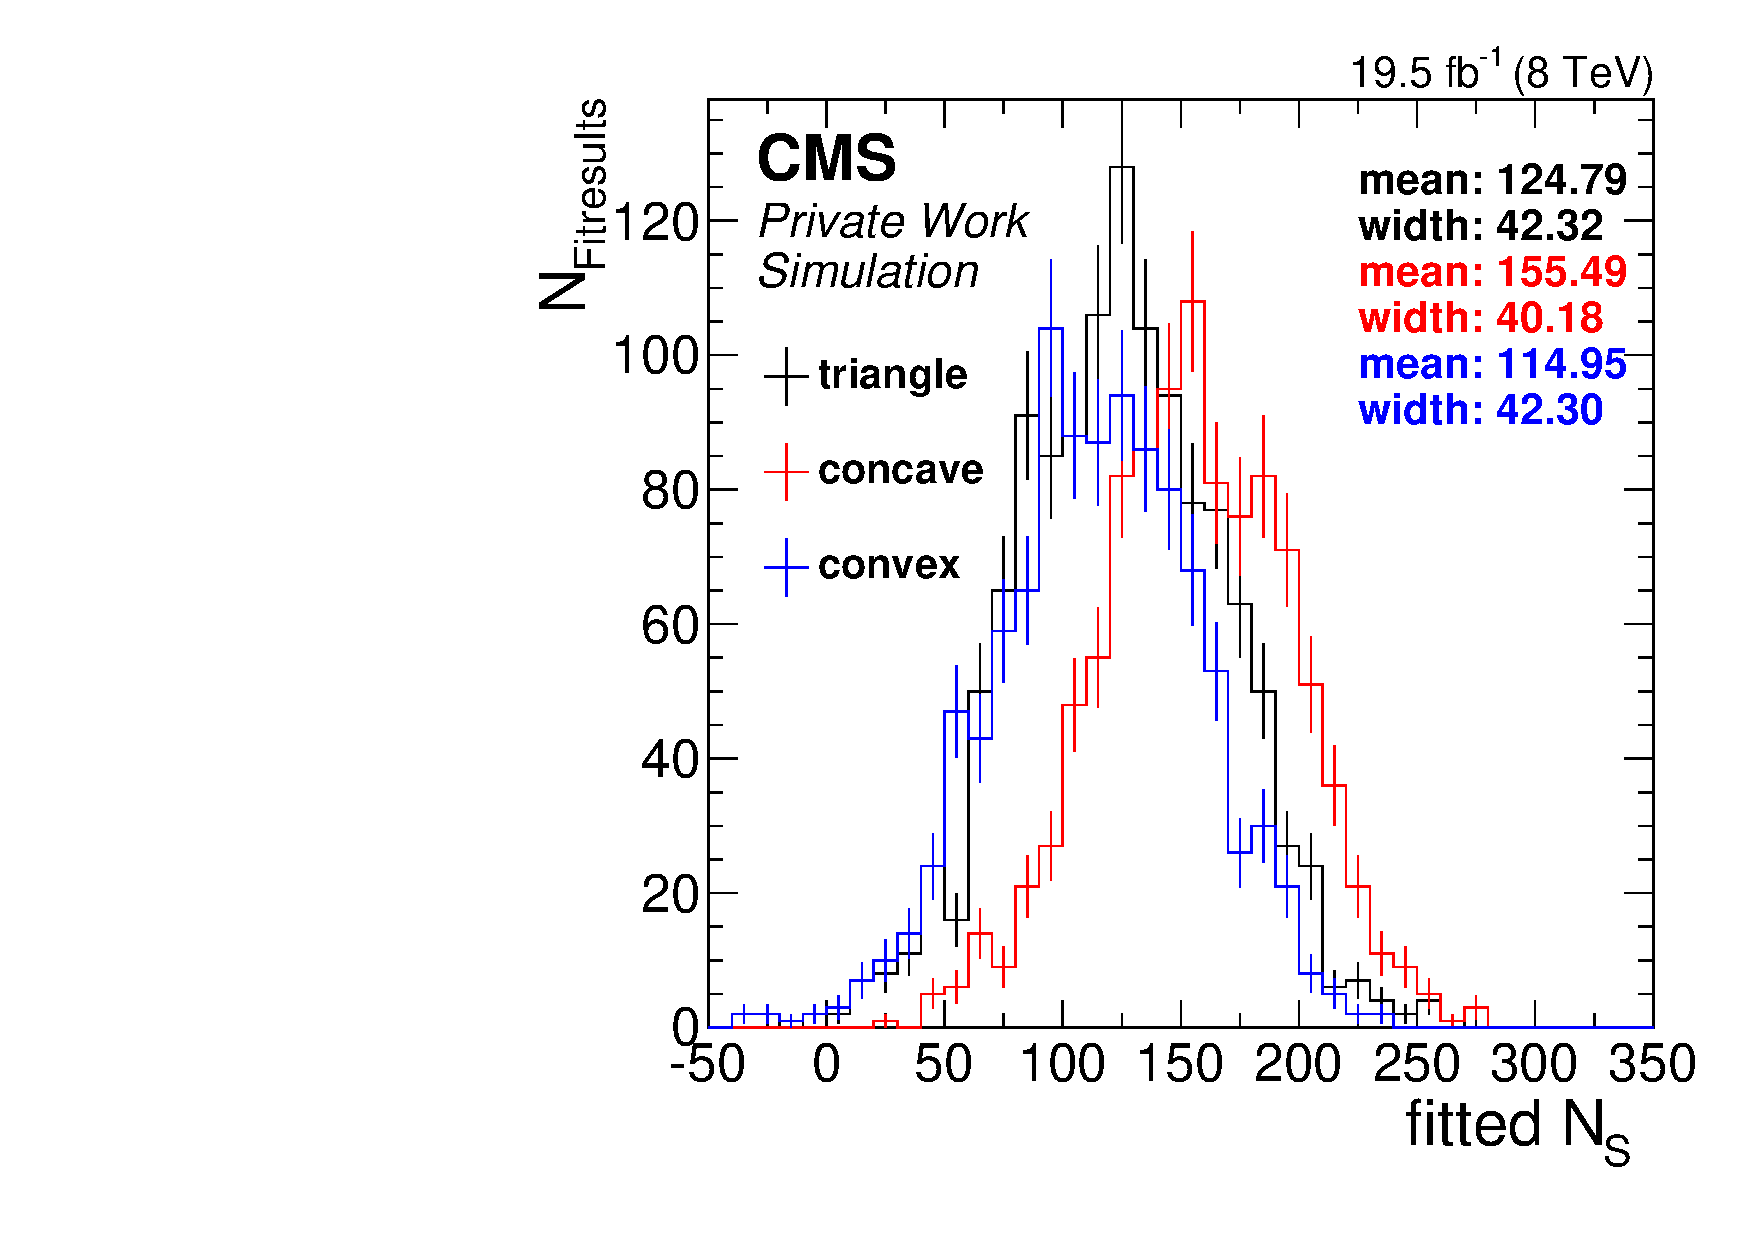
\includegraphics[width=\textwidth]{plots/results/fit/toyResults/nSPure_shapeBias.pdf}
  \end{minipage}
  \begin{minipage}[t]{0.49\textwidth}
    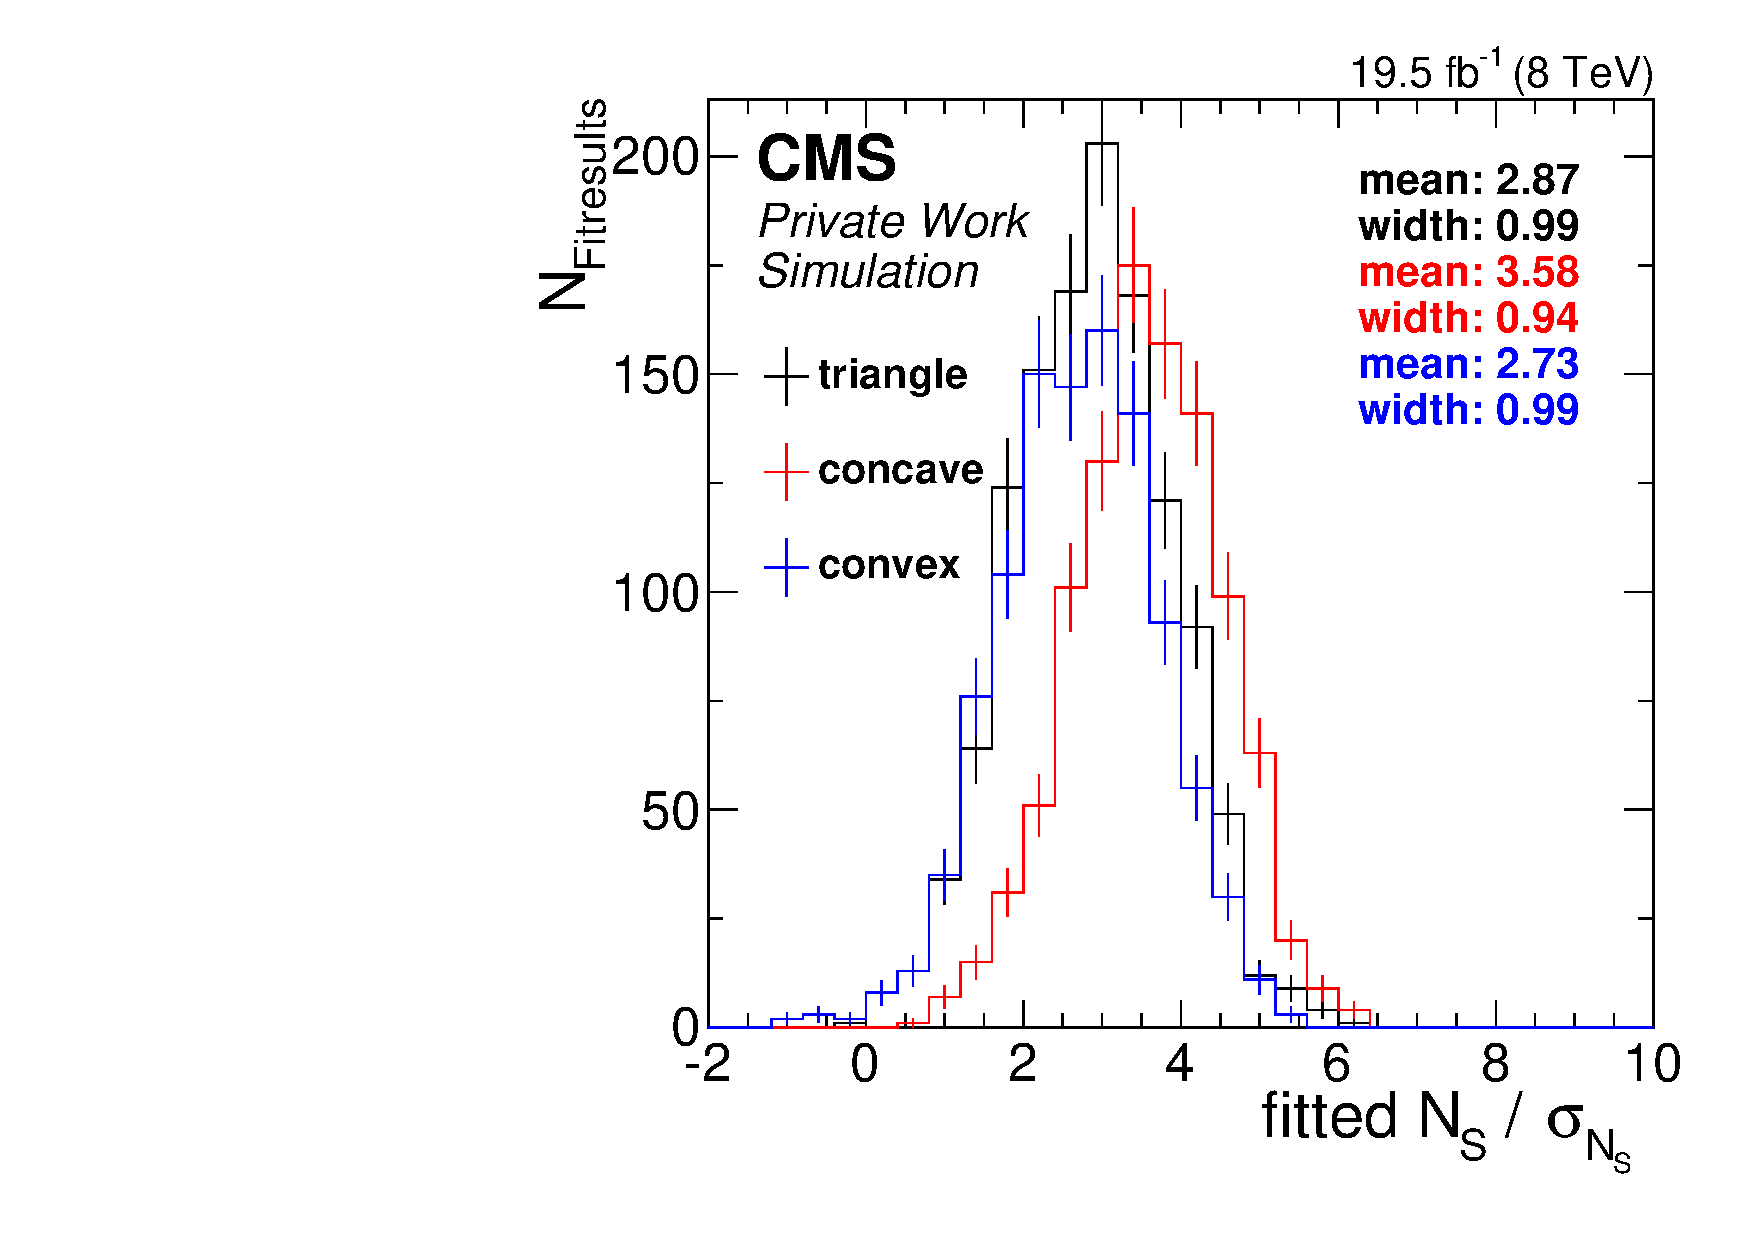
\includegraphics[width=\textwidth]{plots/results/fit/toyResults/nS_shapeBias.pdf}
  \end{minipage}
  \begin{minipage}[t]{0.49\textwidth}
    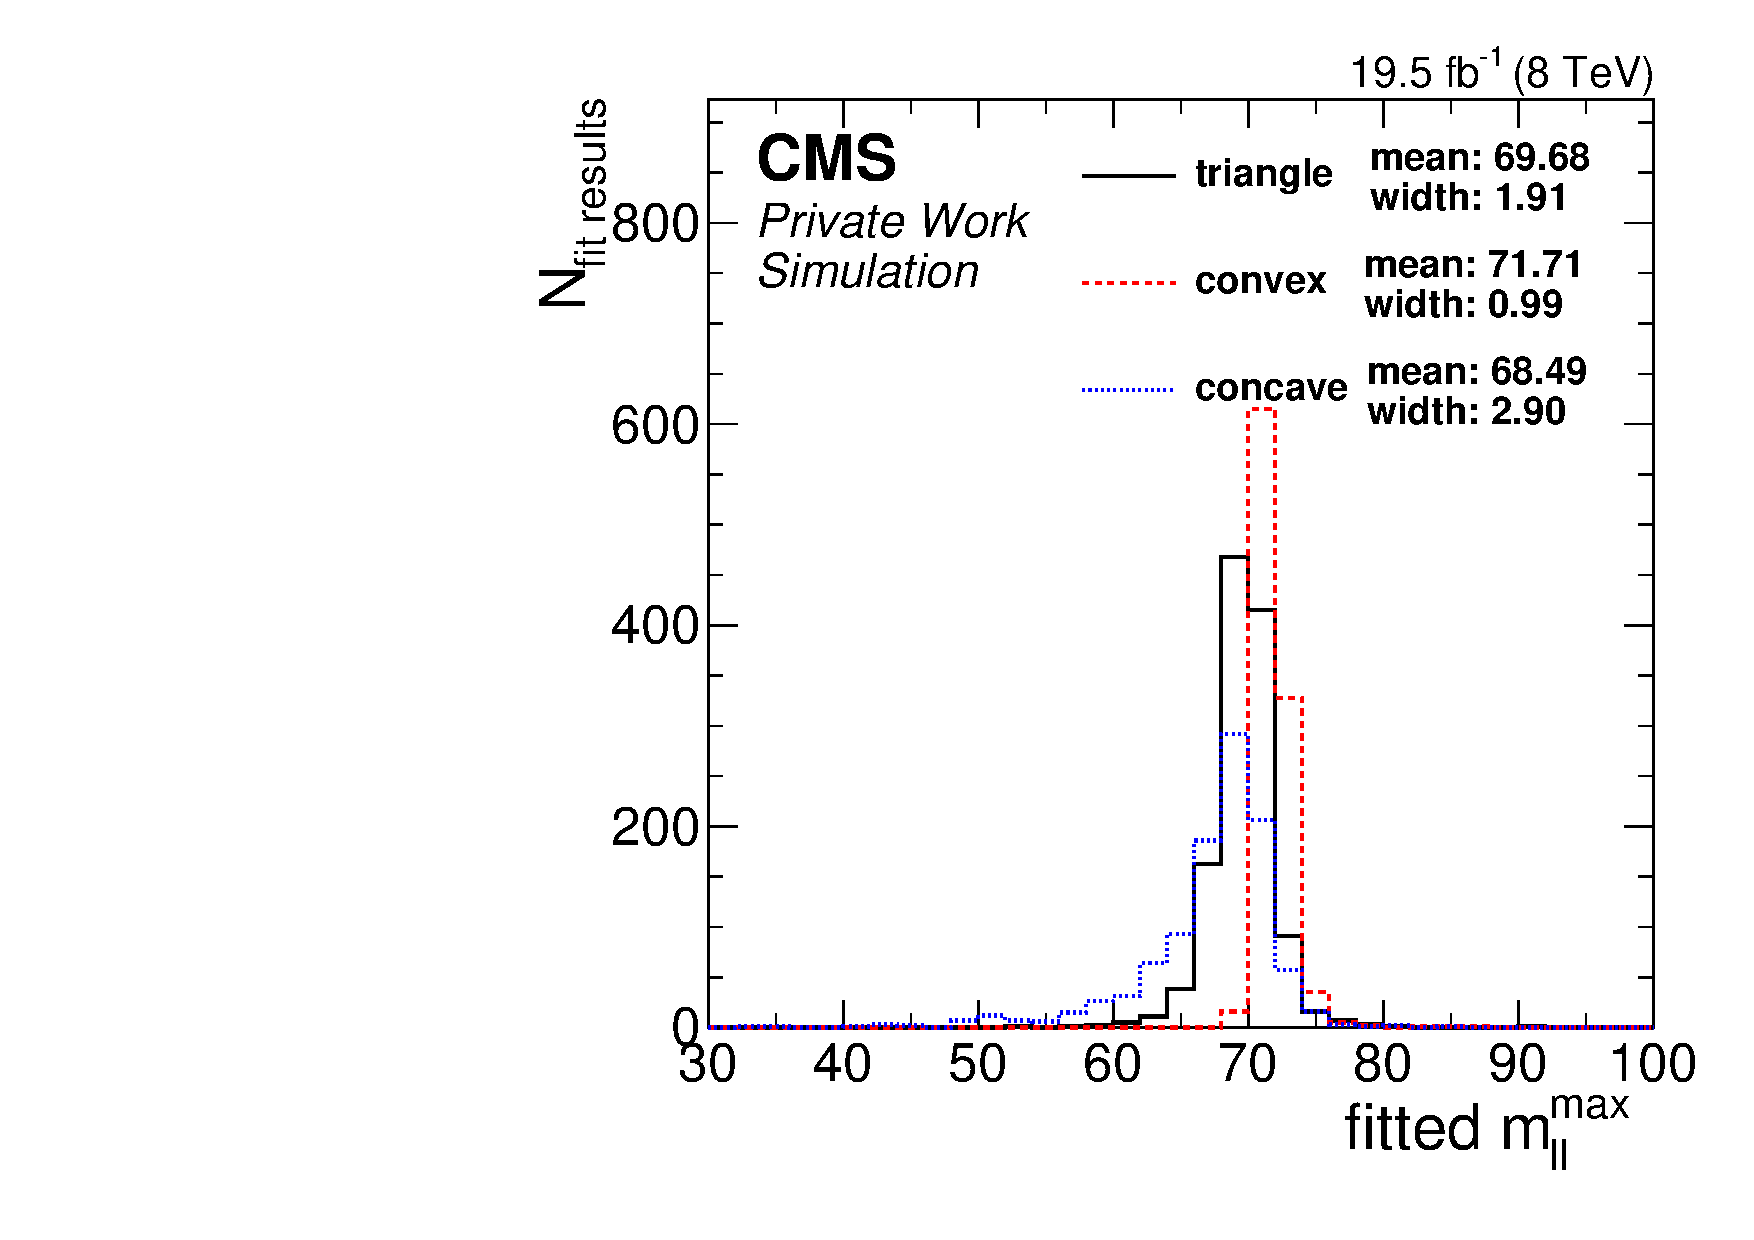
\includegraphics[width=\textwidth]{plots/results/fit/toyResults/m0_shapeBias.pdf}
  \end{minipage}
  \begin{minipage}[t]{0.49\textwidth}
    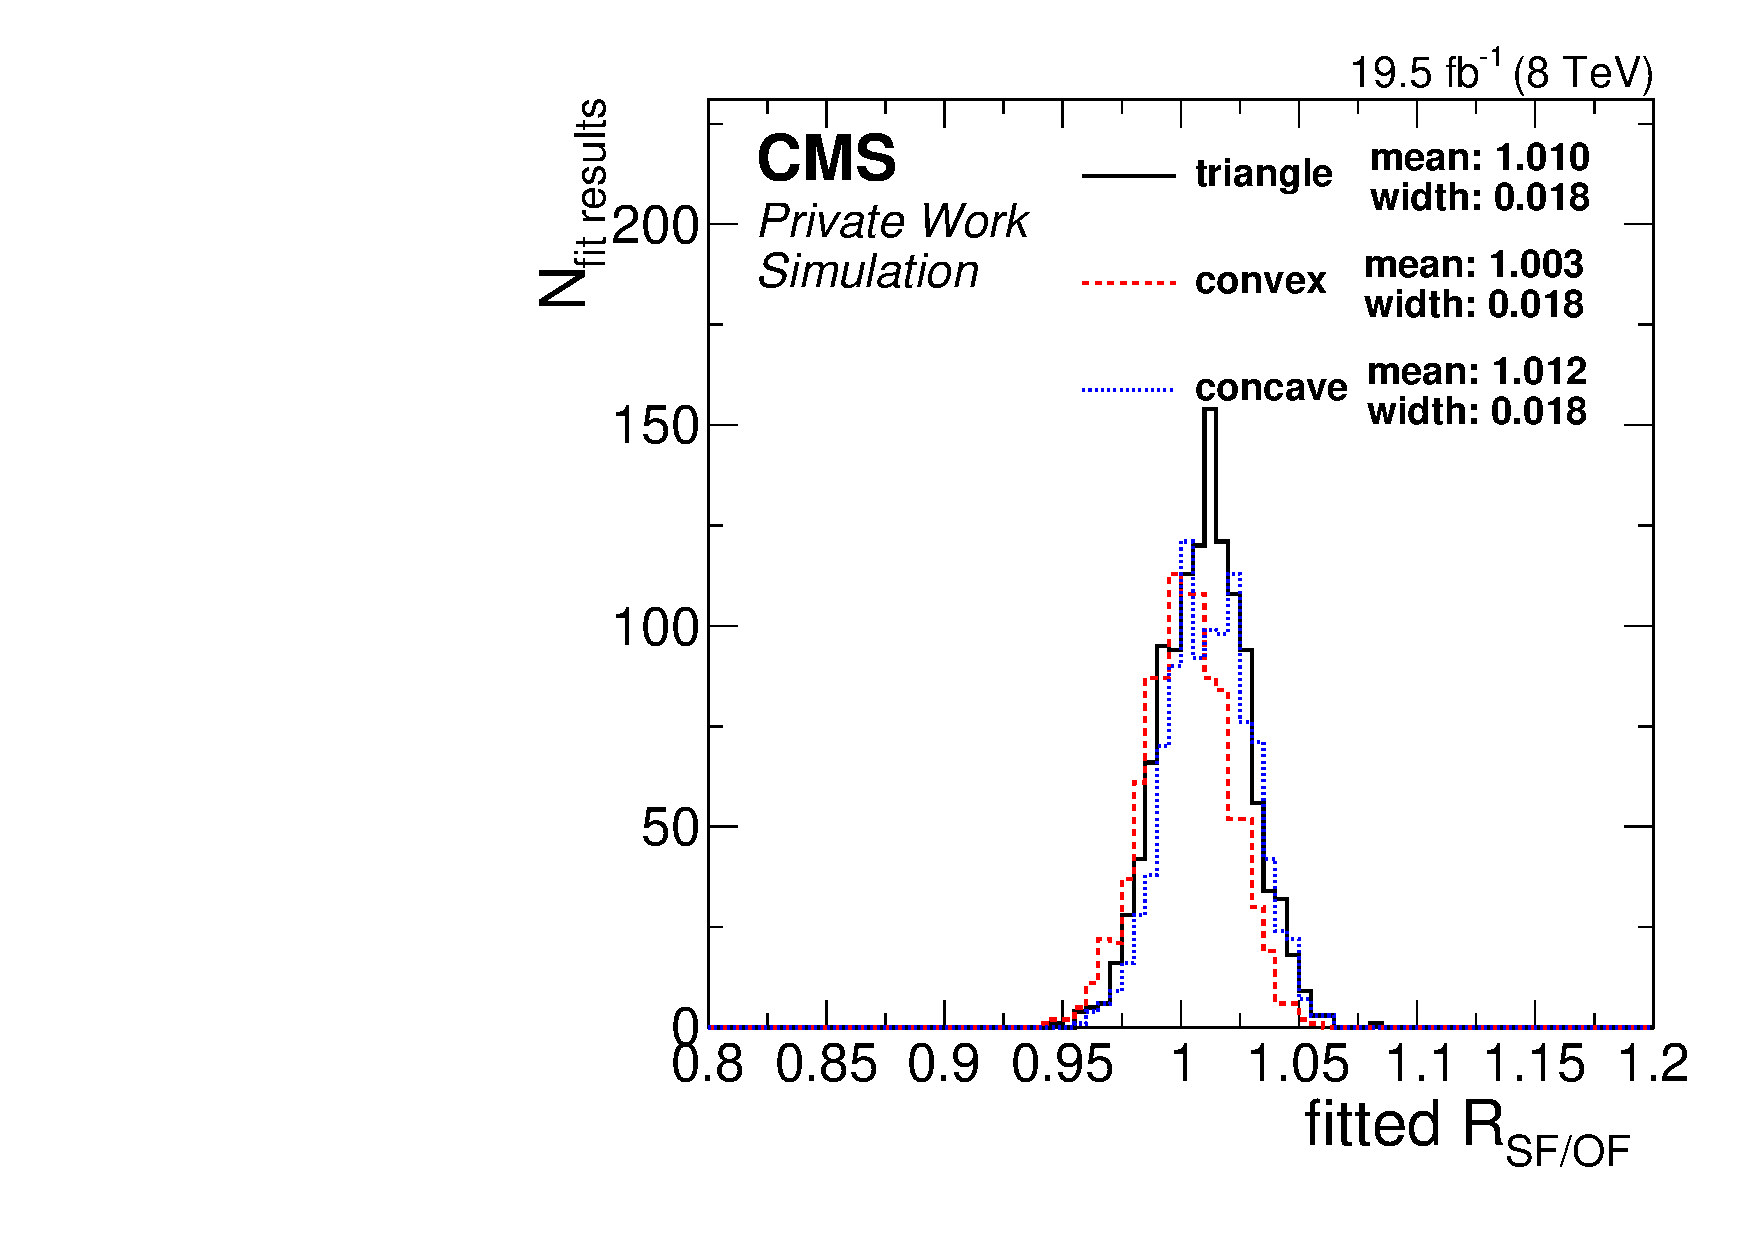
\includegraphics[width=\textwidth]{plots/results/fit/toyResults/rSFOF_shapeBias.pdf}
  \end{minipage}
  \caption{Distribution of fit observables in toy studies with signals following different distributions. Toys are generated using the nominal (black) as well as the concave (red) and convex (blue) signal shape. Shown are the fitted number of signal events in the central region (upper left), the fitted number of signal events divided by the fitted uncertainty in the central region (upper right), the fitted edge position (lower left) and the fitted \Rsfof in the central region (lower right).}
  \label{fig:toys:signalInjectedShapeBias}
\end{figure}
\clearpage
\section{Results}
The result of the fit performed in the signal region on data is shown in Figure~\ref{fig:fit:result}. Shown are the \mll distributions in the SF and OF channels for the central and forward dilepton selection. The quantitative results are shown in Table~\ref{tab:fitResult}. Similar to the counting experiment, an excess of events is observed below the Z boson peak in the central signal region. The best fit value for the position of an edge is found to be $\unit{82.4}{\giga\electronvolt}$, with an signal yield of 140$\pm$43 events. No significant contribution of a signal is found in the forward region, where the fitted signal yield is 1$\pm$22 events. In the central region the fitted value of \Rsfof is slightly larger than the initial value, indicating that the fit absorbs some fraction of the excess into the background prediction. However, the difference is small compared to the fitted uncertainty and the uncertainty on the predicted value. In the forward region, the fitted value is smaller than the initial value, but also this deviation is well within the uncertainties. 


\begin{figure}[!hbp]
  \centering
  \begin{minipage}[t]{0.49\textwidth}
    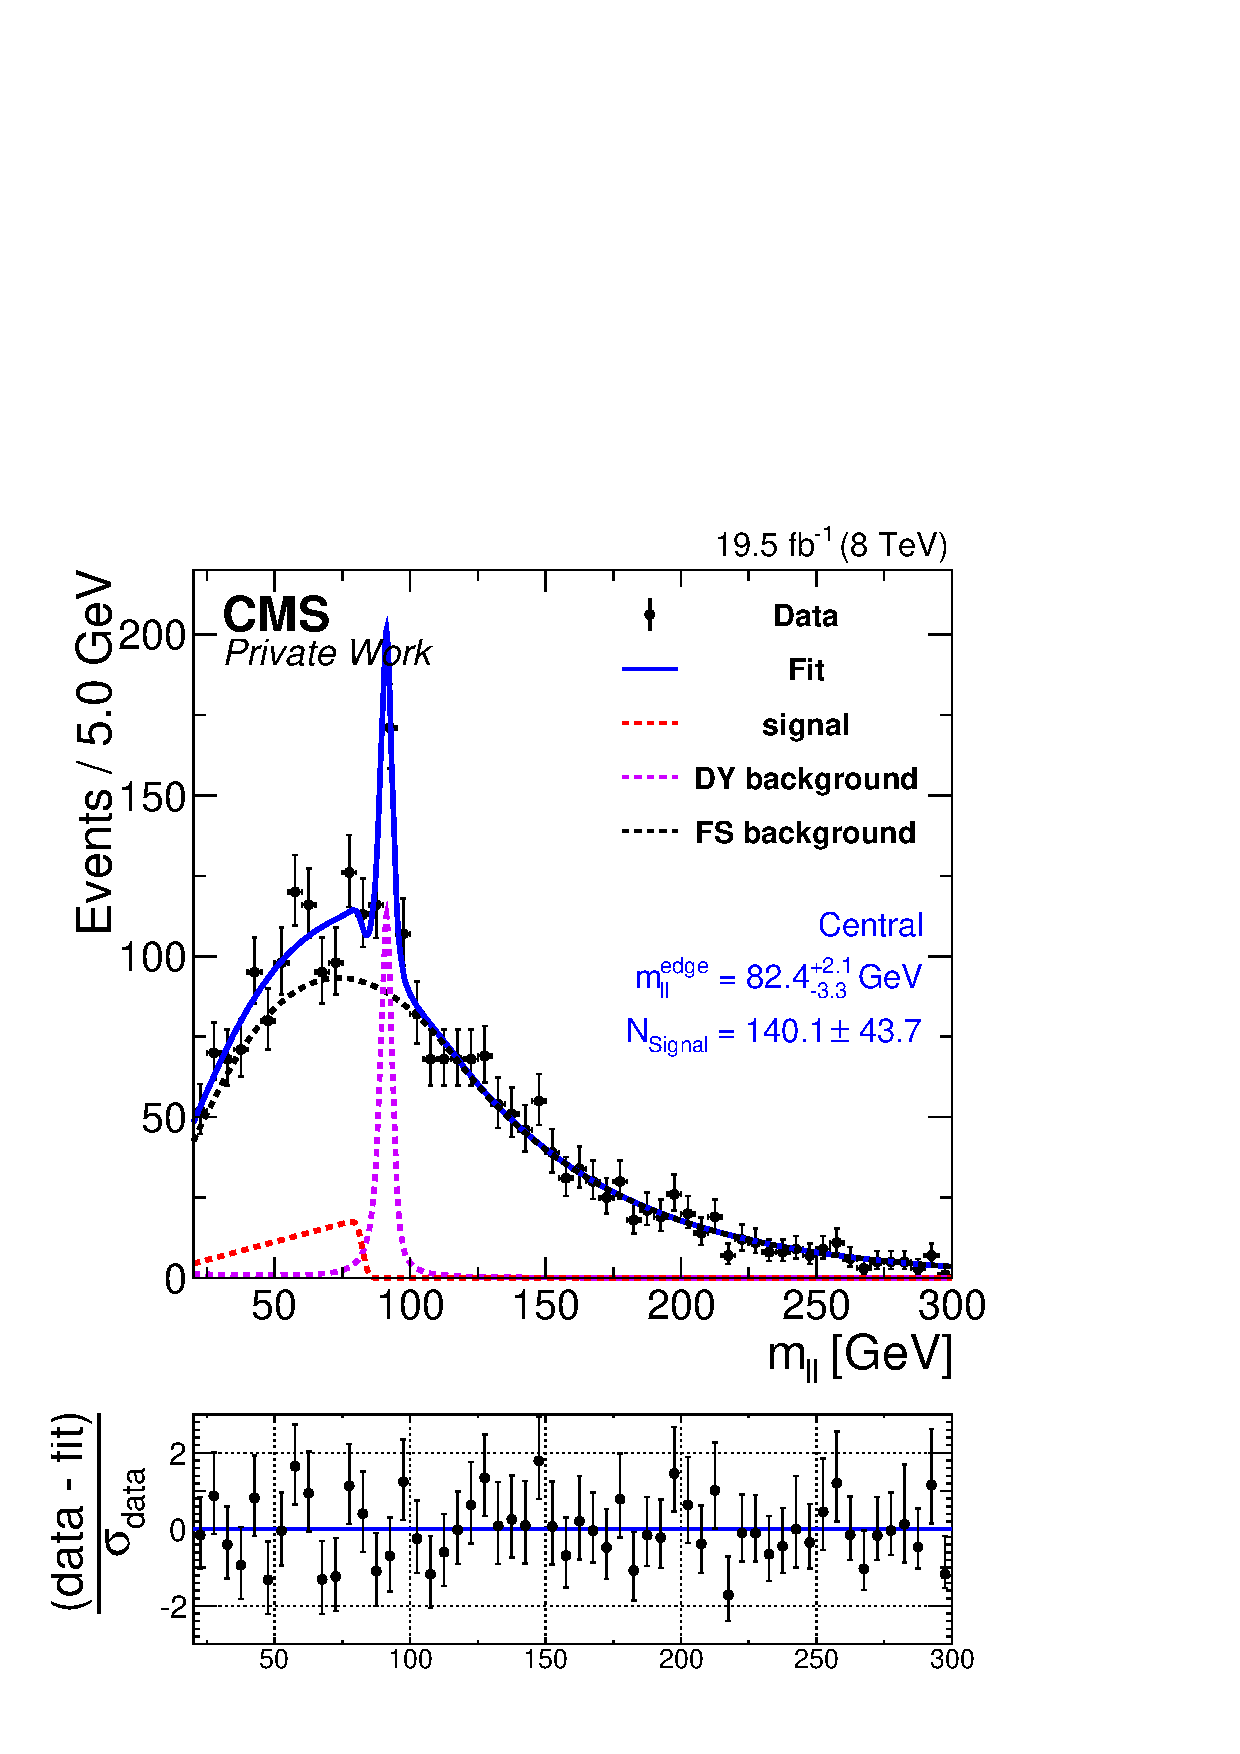
\includegraphics[width=\textwidth]{plots/results/fit/fit2012_ETHTriangle_SignalInclusive_Combined_Full2012_ETHTriangle_Central.pdf}
  \end{minipage}
  \begin{minipage}[t]{0.49\textwidth}
    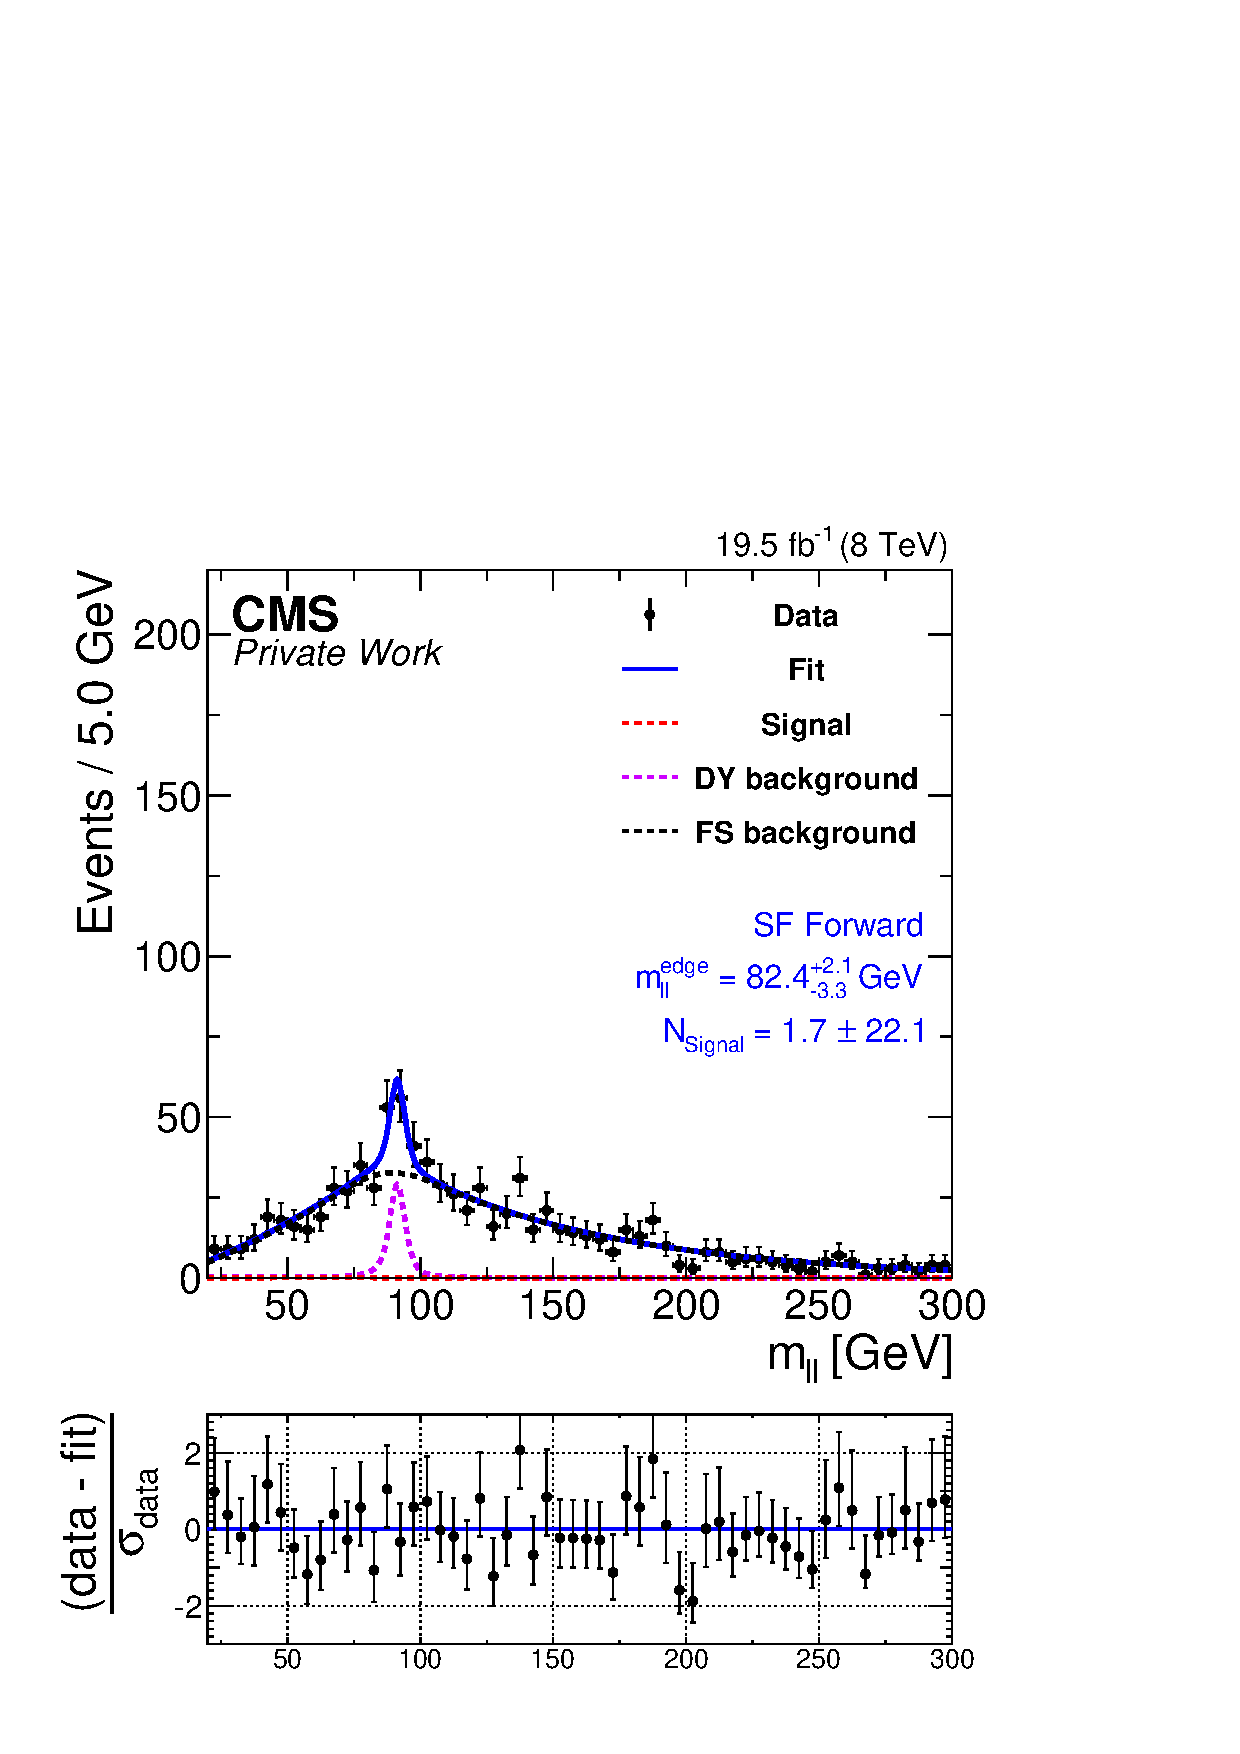
\includegraphics[width=\textwidth]{plots/results/fit/fit2012_ETHTriangle_SignalInclusive_Combined_Full2012_ETHTriangle_Forward.pdf}
  \end{minipage}
  \begin{minipage}[t]{0.49\textwidth}
    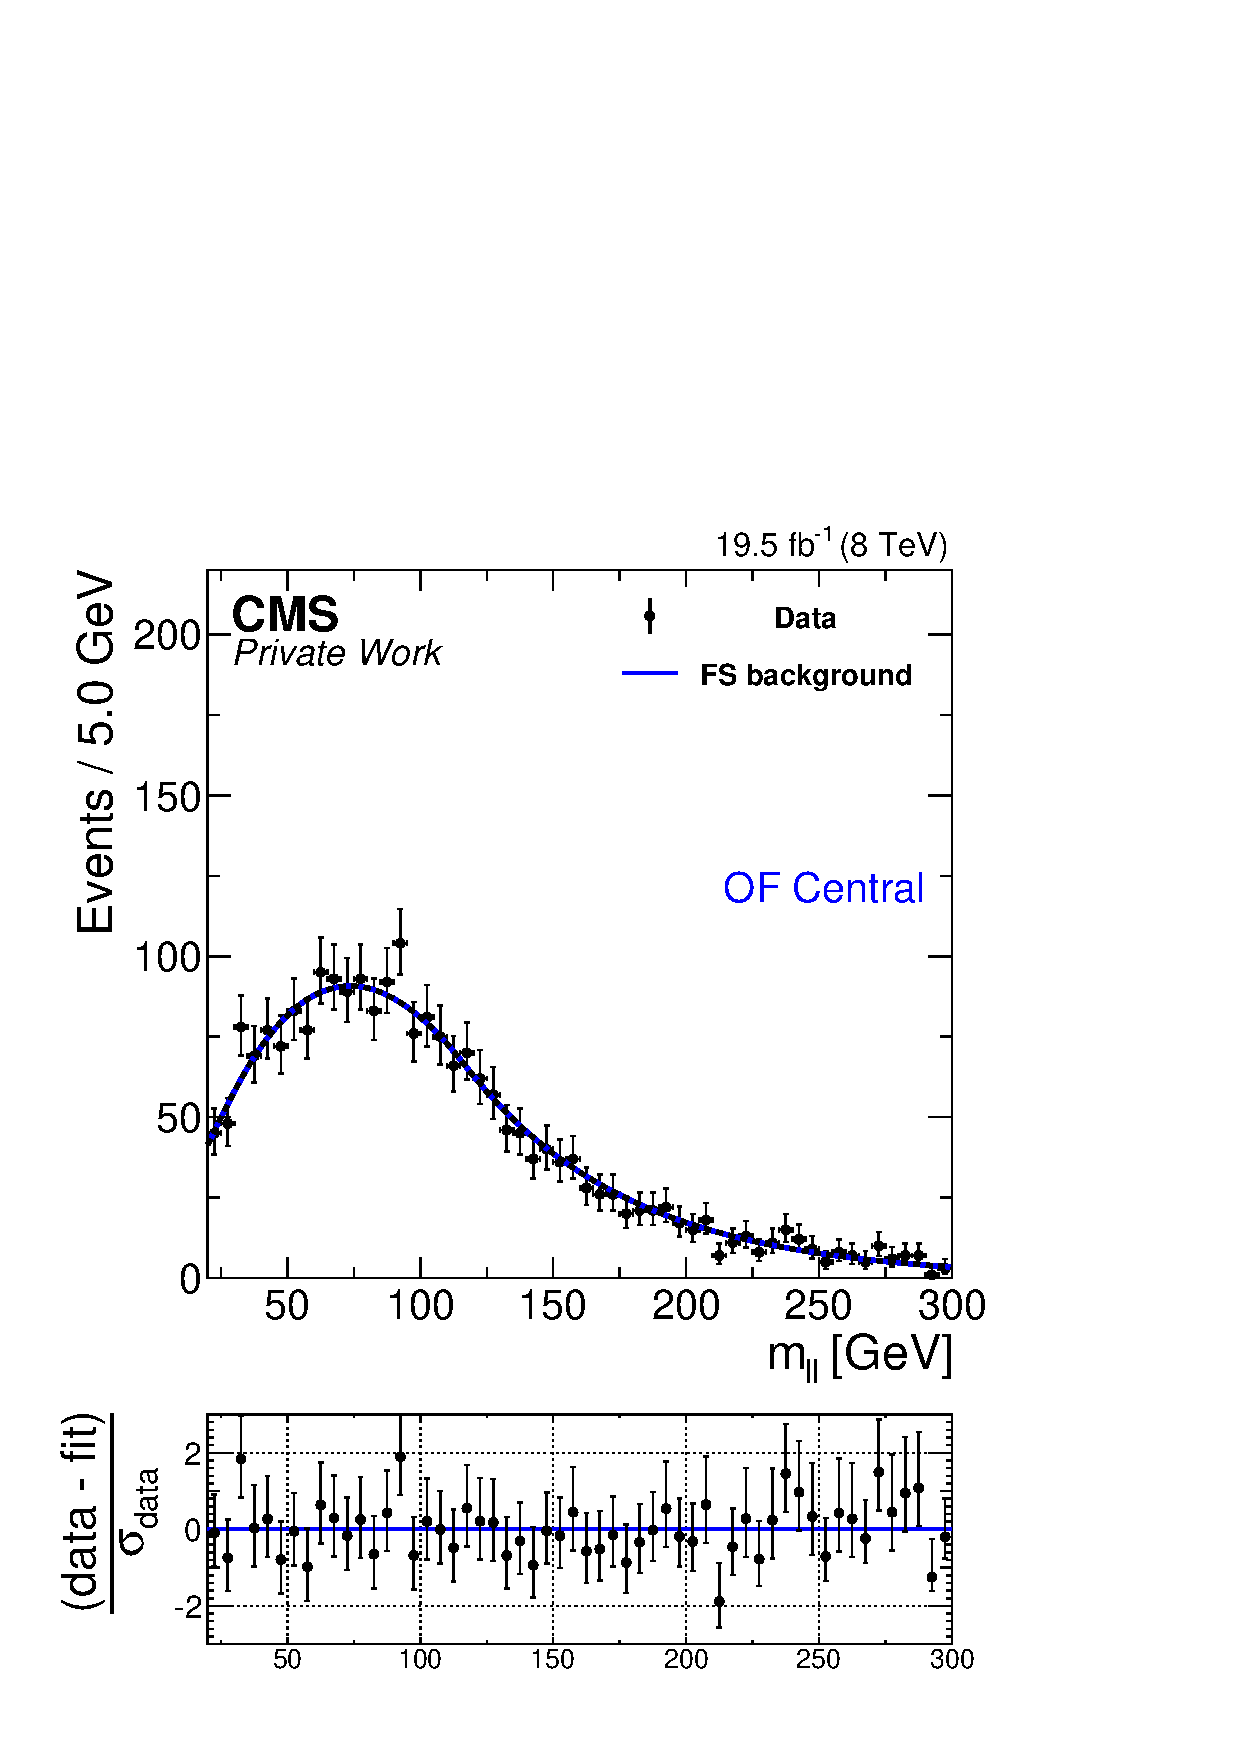
\includegraphics[width=\textwidth]{plots/results/fit/fit2012OFOS_ETHTriangle_SignalInclusive_Combined_Full2012_ETHTriangle_Central.pdf}
  \end{minipage}
  \begin{minipage}[t]{0.49\textwidth}
    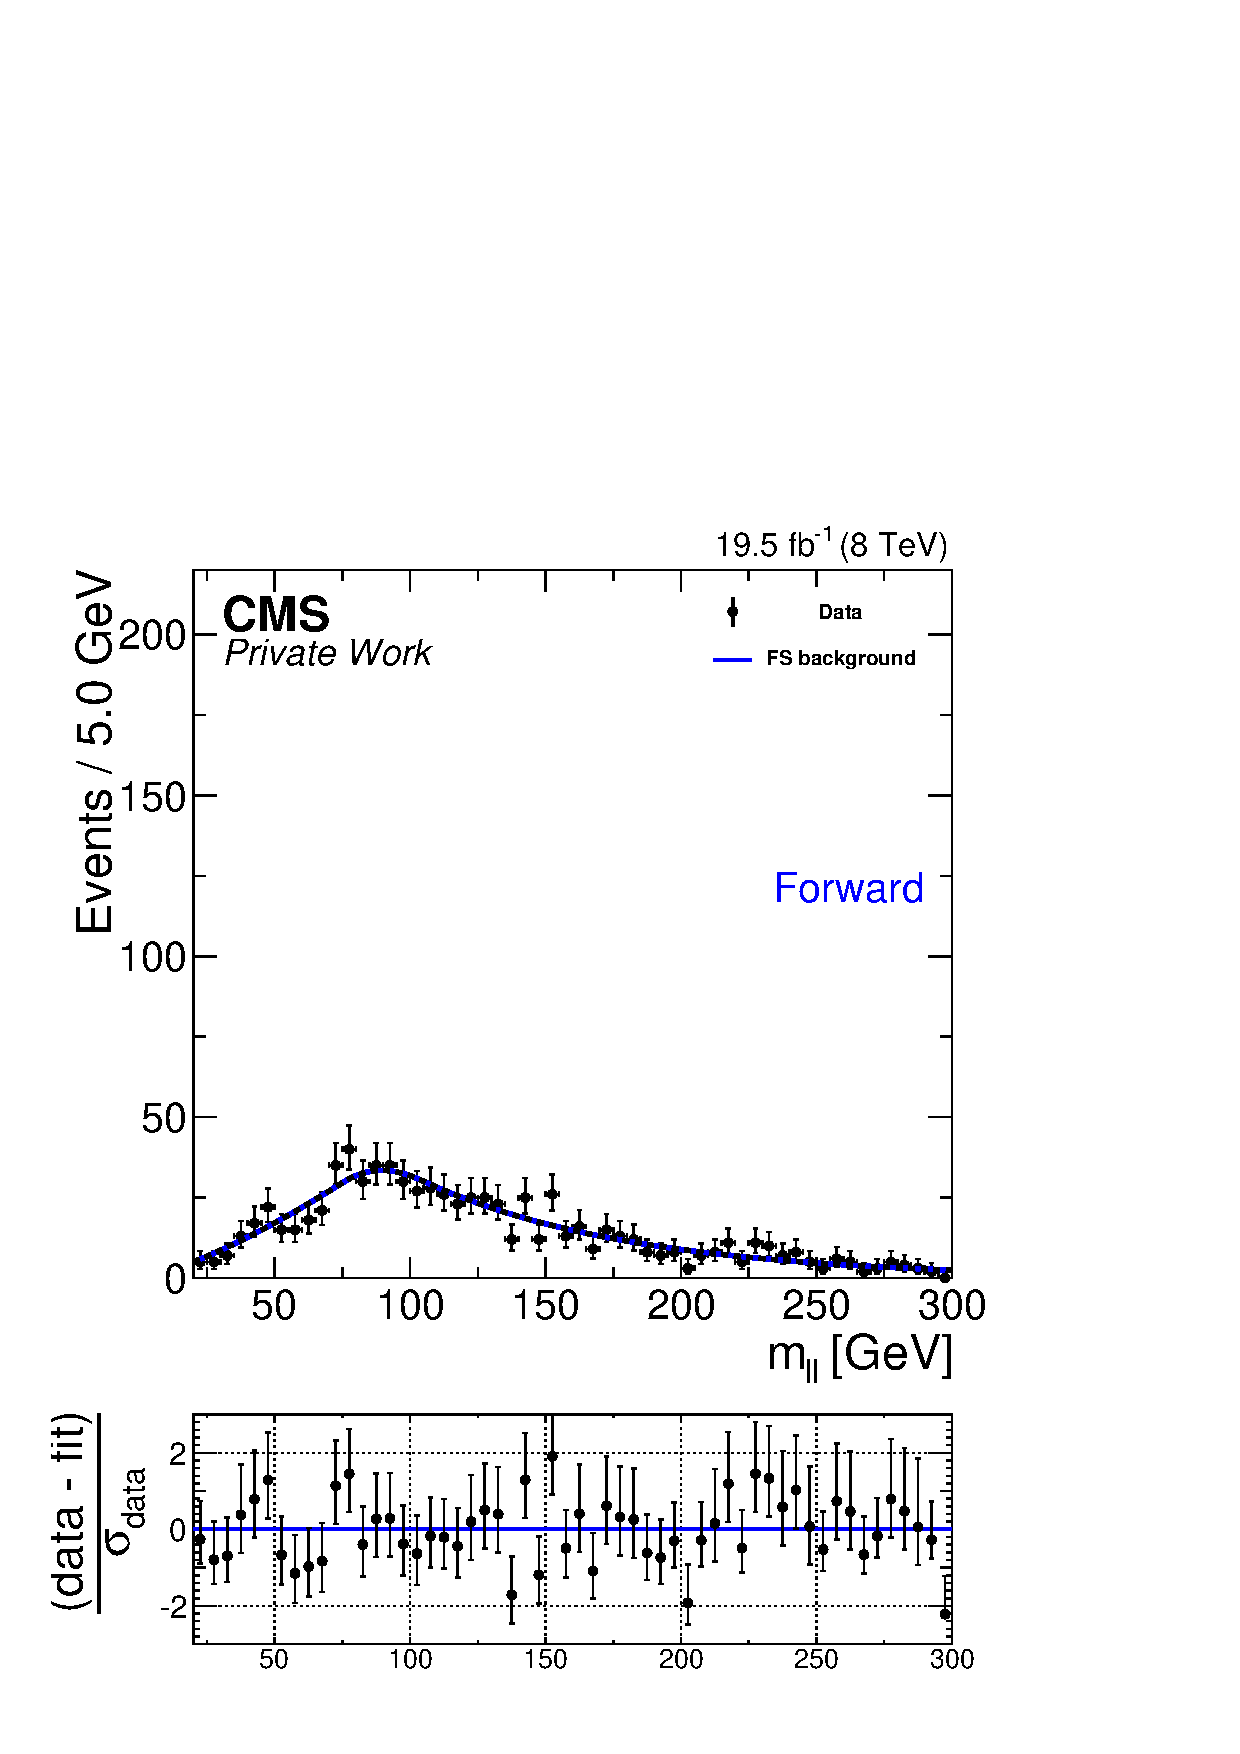
\includegraphics[width=\textwidth]{plots/results/fit/fit2012OFOS_ETHTriangle_SignalInclusive_Combined_Full2012_ETHTriangle_Forward.pdf}
  \end{minipage}
  \caption{Fit results in the signal region. Shown are the \mll distributions in SF (top) and OF (bottom) events for the central (right) and forward (left) dilepton selection. The fit is shown as a solid blue line while the different components are shown as dashed line, the signal model in red, the Drell--Yan model in violet and the flavour-symmetric model in black.}
  \label{fig:fit:result}
\end{figure}


\begin{table}[hbtp]
 \renewcommand{\arraystretch}{1.3}
 \setlength{\belowcaptionskip}{6pt}
 \centering
 \caption{Results of the fit in search for a kinematic edge in the signal region.
     }
  \label{tab:fitResult}
  \begin{tabular}{l| cc }
    \hline
    \hline
                                &  Central        & Forward \\ 

    \hline
        Drell--Yan background       &  170$\pm$23                   & 55$\pm$15  \\
        Flav. Sym. background in OF       &  2293$\pm$45                   & 792$\pm$25  \\
        \Rsfof       &  1.024$\pm$0.027                   & 1.012$\pm$0.042  \\
        signal events       &  140$\pm$44                   & 2$\pm$22  \\
        $m_{\ell\ell}^{edge}$ [GeV]       &  \multicolumn{2}{c}{$82.4^{+2.1}_{-3.3}$}  \\

\hline
\        local significance [$\sigma$]       &  \multicolumn{2}{c}{2.5 }  \\

    \hline
    \hline    
  \end{tabular}
\end{table}




A scan of the log-likelihood as a function of the edge position $m_{\ell\ell}^{egde}$ is shown in Figure~\ref{fig:fit:likelihoodScan}. The values have been shifted to set the minimum to zero. The curve exhibits a sharp drop at the best fit value for $m_{\ell\ell}^{egde}$, which is indeed the global minimum over the considered mass range. 

\begin{figure}[htbp]
\centering
  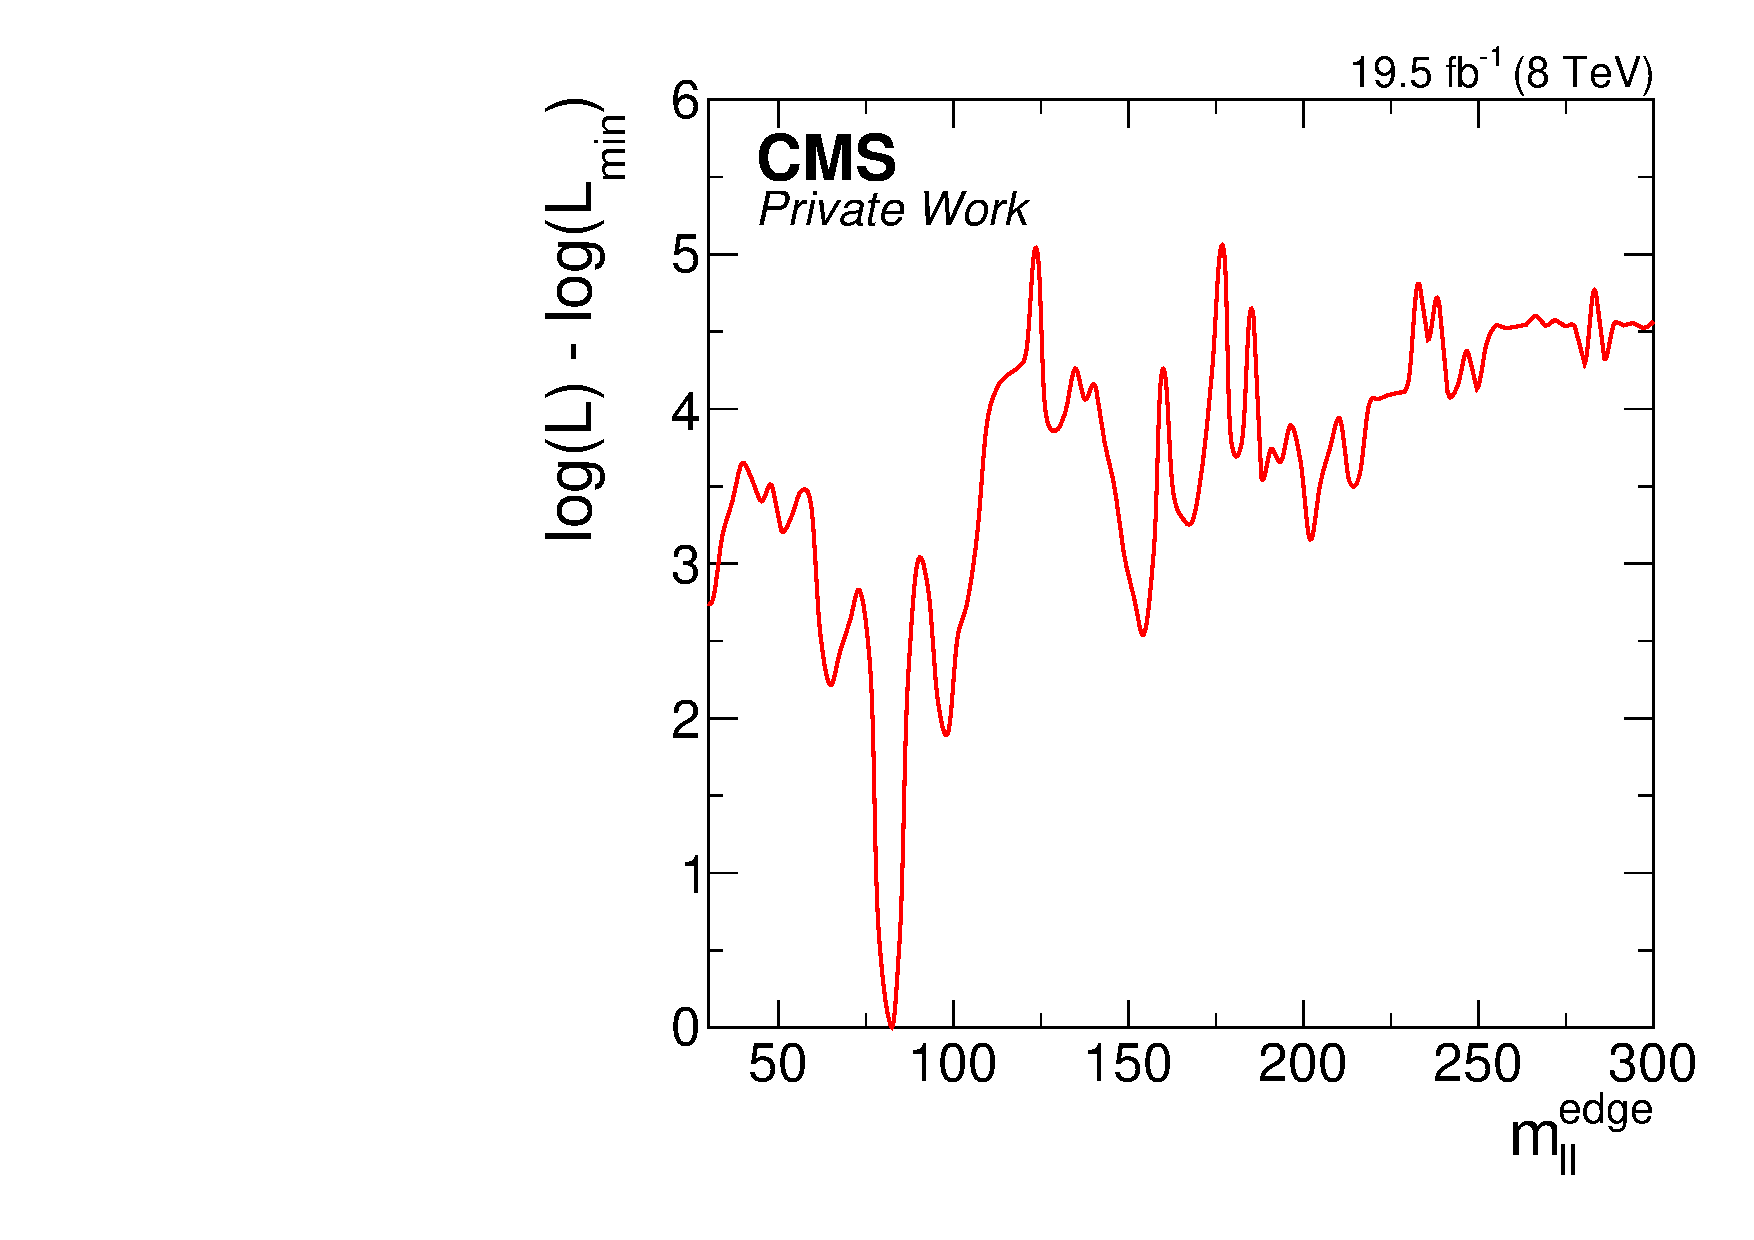
\includegraphics[width=0.6\textwidth]{plots/results/fit/signal.pdf}
\caption{Scan of the observed log-likelihood in the signal region subtracted by the minimal value as a function of $m_{\ell\ell}^{max}$.}
\label{fig:fit:likelihoodScan}
\end{figure}

The local fit significance is calculated applying Wilk's Theorem~\cite{wilks1938}, which states that the distribution of $-2(log(L_1)-log(L_0))$ ($-2\Delta(log(L))$ in short) is distributed as a $\chi^2$ distribution with n degrees of freedom, where n is the number of free parameters of the signal model and $L_0$ and $L_0$ are the likelihood values of the background only and the signal plus background hypothesis. The p-Value of a result can then be obtained by simply integrating this $\chi^2$ distribution for values larger than the one observed in data. However, Wilk's Theorem does not hold in cases where one parameter of the signal model is not defined in the background only model. This is the case for signal models including the position of a bump, or in this case an edge, as a free parameter. 

The applicability of Wilk's theorem is demonstrated using the toy fits described in Section~\ref{sec:toysWO}. They can also be used to calculate directly the significance and are also able to provide global results.
Considered are toy dataset without signal injection. The fits are performed both with a floating edge position and fixed \mlledge. Figure~\ref{fig:toySignif} shows the resulting distributions of $-2\Delta(log(L))$ for the both scenarios. The $\chi^2$ distributions for 2 and 3 degrees of freedom are shown for illustration. In the case of the fixed edge the results of the fits follow the distribution for 2 degrees of freedom, as expected from the presence of $N_{S}^{\text{central}}$ and $N_{S}^{\text{forward}}$. This proves the applicability of Wilk's theorem for this case. The floating edge position however clearly does not simply act as an additional degree of freedom as the distribution of the toy results is shifted to higher values of $-2\Delta(log(L))$, indicating that Wilk's theorem does indeed not hold for this type of models.
The p-Value of the fit result is in both cases given by the fraction of results for with $-2\Delta(log(L))$ exceeds the one observed on data. The result for a fixed edge can then be interpreted as a local p-Value while the ones for a floating edge gives a global p-Value taking into account the so called ``Look-elsewhere-effect''~\cite{GrossVittels}. However, as the signal yield is allowed to be negative, the resulting p-Values have to be reduced by a factor of two to take into account that we only consider positive signals to have physical meaning~\cite{GrossVittels}. This corrected p-Value is translated into a significance interpreting it as the one-sided tail probability of a unit Gaussian. The resulting uncorrected p-Values are $0.012^{+0.004}_{-0.003}$, corresponding to $2.5\sigma$, in the local and $0.091^{+0.009}_{-0.009}$, corresponding to $1.7\sigma$, in the global case.

\begin{figure}[htbp]
\centering
  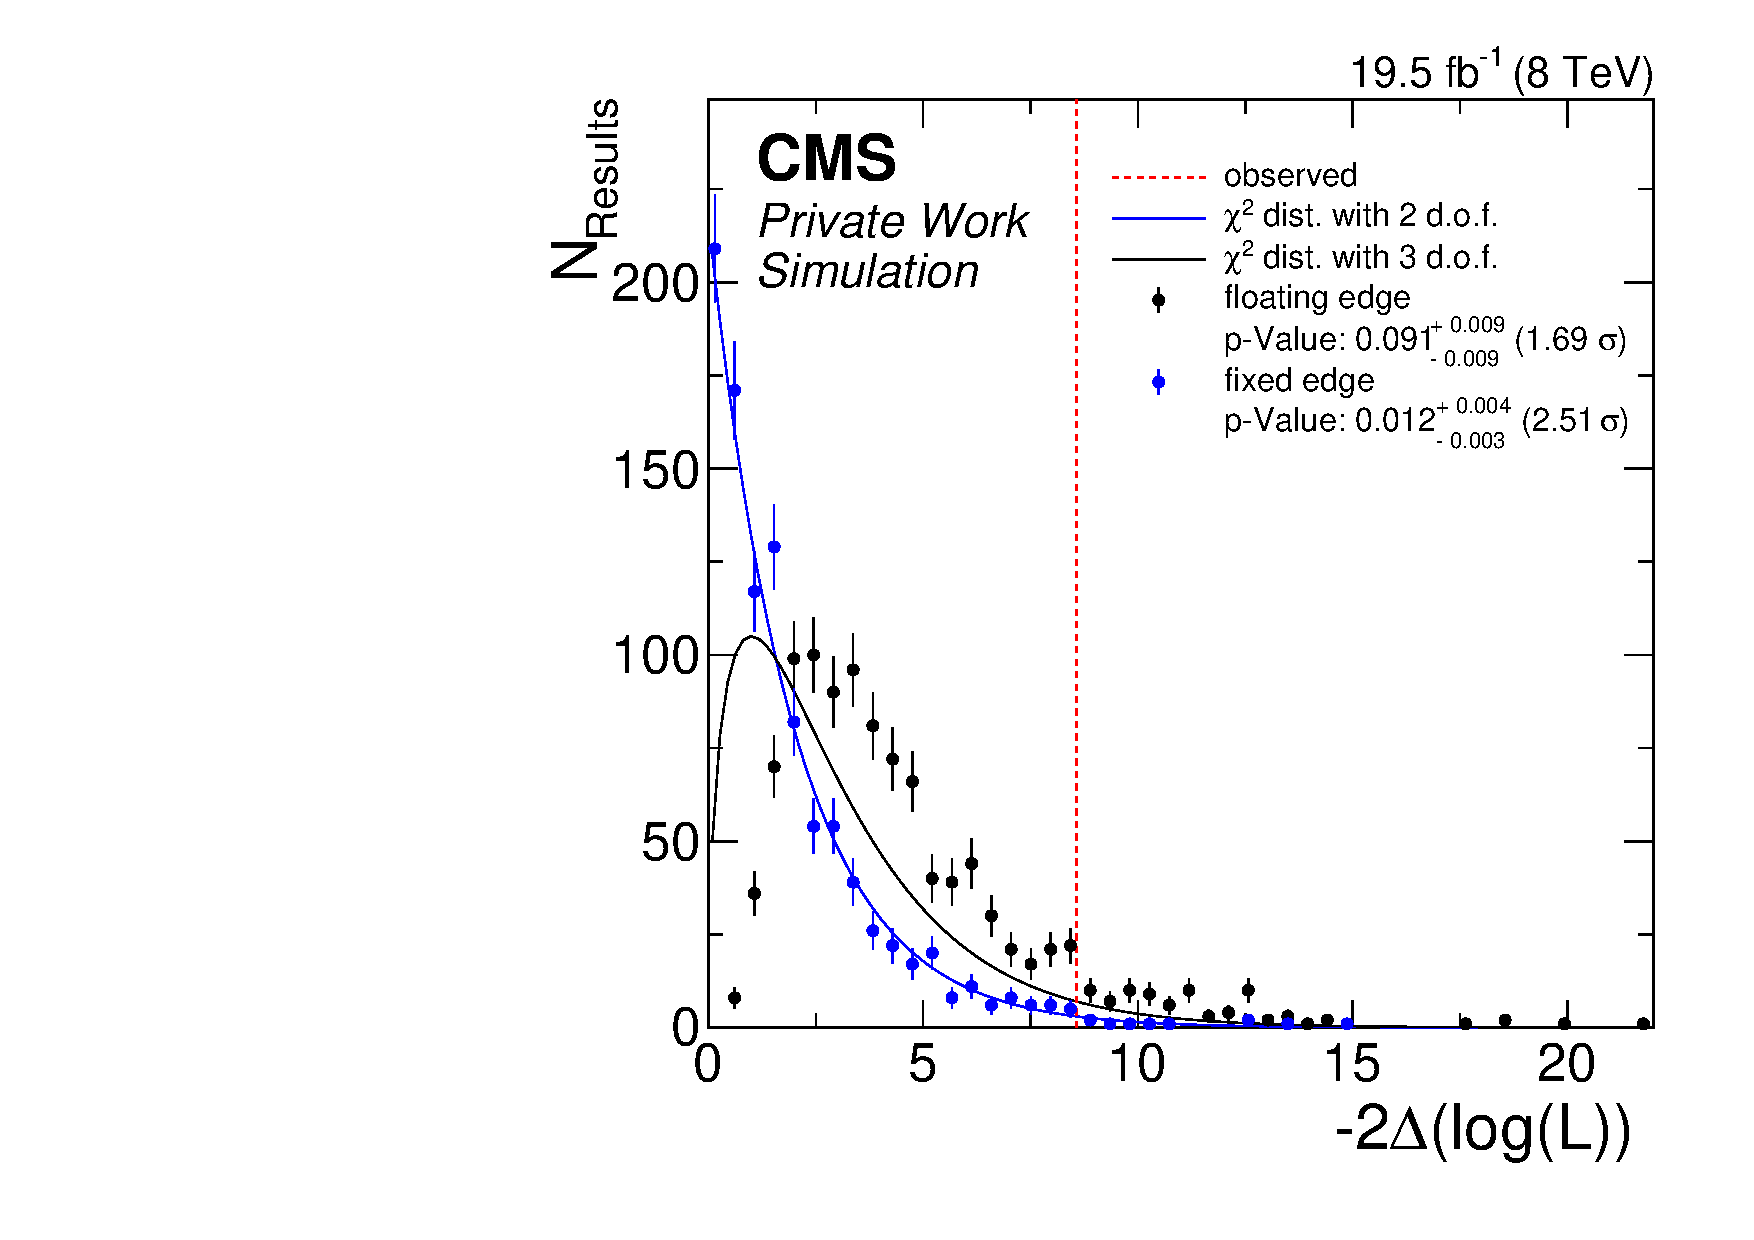
\includegraphics[width=0.6\textwidth]{plots/results/fit/toyResults/significanceStudy_BackgroundOnly.pdf}
\caption{Calculation of the fit significance using background only toy MC. Shown are the distribution of $-2\Delta(log(L))$ for fits with floating (black) and fixed (blue) edge position. Also shown are $\chi^2$ distributions for 2 (blue) and 3 (black) degrees of freedoms. The dashed red line indicates the value of $-2\Delta(log(L))$ observed on data in case of a floating edge.}
\label{fig:fit:toySignif}
\end{figure}

As the applicability of Wilk's theorem has been established, local p-Values and significances can be calculated analytically from the $\chi^2$ function for two degrees of freedom. The p-Value is defined as the integral of the function above the value of $-2\Delta(log(L))$ observed on data for a fit performed with fixed edge position. Performing such a fit on data with \mlledge set to the observed value, this results in a p-Value of 0.014, corresponding to a significance of $2.5\sigma$. This is well compatible with the result observed using toy MC. The local significances reported in Table~\ref{tab:fitResult} and those discussed in the following are calculated using the analytical calculation as it is much faster and not affected by statistical uncertainties. Also the toys have the small caveat that a different background shape as in the nominal fit is used. 

As further validation of the result on data, the results obtained with different parametrization of the flavour-symmetric background are compared to the nominal result in Table~\ref{tab:fitComparison}. For the sake of clarity, only yields in the central signal region are shown. However, similar agreement is observed also in the forward signal region. In general, there is good agreement between all considered parametrizations. The best agreement is seen in the number of fitted flavour-symmetric events in the OF sample, which is expected as here the fit is mist simple, consisting only of one the shape for flavour-symmetric backgrounds. Good agreement is also observed for $m_{\ell\ell}^{egde}$ and the number of signal events, which are stable against the choice of background model. The most differences are observed for \Rsfof and the yield of the Z model. Here the fit can trade one against the other, depending on the parametrization of the flavour-symmetric background. Here the largest deviations are observed for the shape used in the analysis of the $\unit{7}{\tera\electronvolt}$ dataset. As this shape is known to not satisfactorily described the flavour-symmetric background, it is encouraging to see that the fit result is stable against such biases. The observed local significance is very similar among all analytical parametrizations. In the case of the KDE and the binned parametrization, the shape of the distribution is not free in the fit, as discussed above, excluding the statistical uncertainty of the OF sample from the fit and resulting in an systematically larger local significance. 


\begin{table}[hbtp]
 \renewcommand{\arraystretch}{1.3}
 \setlength{\belowcaptionskip}{6pt}
 \centering
 \caption{Comparison of edge fit results in the signal region for different parametrizations of the flavour-symmetric background. Results are given for the central signal region only. Similar agreement between the parametrization is also observed in the forward signal region.
     }
  \label{tab:fitComparison}
  \begin{tabular}{l| c c c c c c }
    \hline
    \hline
                                &  $N_{DY}$  & $N_{FS}$ & \Rsfof & $N_{S}$ &  $m_{\ell\ell}^{edge}$ [GeV]  & local $\sigma$ \\ 

    \hline
        nominal       &  170$\pm$23  &  2293$\pm$45 &  1.024$\pm$0.027 &  140$\pm$43 &   $82.4^{+2.1}_{-3.3}$      & 2.5  \\
        sum of Gaussians       &  168$\pm$24  &  2292$\pm$44 &  1.023$\pm$0.027 &  146$\pm$50 &   $82.1^{+2.2}_{-3.7}$      & 2.7  \\
        kernel density estimation       &  154$\pm$22  &  2296$\pm$43 &  1.028$\pm$0.026 &  141$\pm$41 &   $81.7^{+2.3}_{-3.4}$      & 3.1  \\
        histogram       &  140$\pm$23  &  2296$\pm$43 &  1.029$\pm$0.026 &  153$\pm$41 &   $83.0^{+1.7}_{-2.4}$      & 3.5  \\
        2011 shape       &  181$\pm$23  &  2290$\pm$43 &  1.020$\pm$0.026 &  146$\pm$46 &   $82.8^{+1.9}_{-2.5}$      & 2.7  \\

    \hline
    \hline    
  \end{tabular}
\end{table}




To compare the fit result with that of the counting experiment, the fitted event yields in the low-mass region for central dilepton events have been derived. They are shown in Table~\ref{fig:fit:resultLowMass}, together with the background predictions and observed yield of the counting experiment in that region. Also the fitted yield for Drell--Yan backgrounds  in the on-Z region is compared to the prediction. The fitted yield exceeds that of the prediction by 26 events, a difference that is well covered by the uncertainties of the fit and the prediction. In the low-mass region good agreement between counting experiment and fit is observed, also. The Drell--Yan background is again fitted higher than expected from the prediction, as the ratio between the off-shell component and the peak is fixed and the normalization of this model is determined dominantly on the Z boson peak. In the fit the contribution of flavour-symmetric backgrounds is increased, caused by the increased value of \Rsfof. This is reflected in a signal yield that is lower by 11 events. For all considered components the use of shape information has allowed for reduced uncertainties on the event yields, most notably on the yield for flavour-symmetric backgrounds. 


\begin{table}[hbtp]
 \renewcommand{\arraystretch}{1.3}
 \setlength{\belowcaptionskip}{6pt}
 \centering
 \caption{Comparison of the fit result and the result of the counting experiment in the low mass region for central leptons. The probability density functions contributing to the fit model are integrated in the region $20 < \mll < 70$\GeV to obtain the fitted yields in this interval. Also, the yield in the on-\Z region is calculated and compared to the prediction. 
     }
  \label{tab:fitResultLowMass}
  \begin{tabular}{l| cc }
    \hline
    \hline
                                &  Fit        & Counting experiment \\ 

    \hline
    \multicolumn{3}{c}{on-\Z region} \\ 

    \hline
        Drell--Yan background       &  145$\pm$19                   & 119$\pm$21  \\

\hline
    \multicolumn{3}{c}{low-mass region} \\ 

    \hline
        Drell--Yan background       &  10$\pm$1                   & 8$\pm$2  \\
        Flav. Sym. background       &  760$\pm$14                   & 746$\pm$37  \\
        signal events       &  98$\pm$30                   & 109$\pm$48  \\

    \hline
    \hline    
  \end{tabular}
\end{table}


